% R00 17.ABR.2018 - Edson Bispo Ferreira. Adaptado por Giovani Fonseca Ravagnani Disperati.
%
%-------------------------------------------------------------------------

\documentclass[
	12pt,				
	oneside,			
	a4paper,			
	english,			
	brazil,			
	]{abntex2ppgsi}

% ---s
% Pacotes básicos 

\usepackage[utf8]{inputenc}		% Codificacao do documento (conversão automática dos acentos)
\usepackage{lastpage}			% Usado pela Ficha catalográfica
\usepackage{indentfirst}		      % Indenta o primeiro parágrafo de cada seção.
\usepackage{color}				% Controle das cores
\usepackage{graphicx}		 	% Inclusão de gráficos
\usepackage{microtype} 			% para melhorias de justificação
\usepackage{pdfpages}            %para incluir pdf
\usepackage{algorithm}			%para ilustrações do tipo algoritmo
\usepackage{mdwlist}			%para itens com espaço padrão da abnt
\usepackage[noend]{algpseudocode}			%para ilustrações do tipo algoritmo
\usepackage{quoting}			% pacote de citações (quotes)
\usepackage{setspace}			% pacote singlespace, para citações
\usepackage[Symbol]{upgreek}    %pacote para letras gregas maiúsculas
\usepackage{siunitx}		
\usepackage{multirow}	
\usepackage{amsmath}
\usepackage{float}
\usepackage{blindtext}
\usepackage{adjustbox}

% ---
% Pacotes de citações
% ---
\usepackage[brazilian,hyperpageref]{backref}	 % Paginas com as citações na bibl
\usepackage[alf]{abntex2cite}	% Citações padrão ABNT

% --- 
% CONFIGURAÇÕES DE PACOTES
% --- 

% ---
% Configurações do pacote backref
% Usado sem a opção hyperpageref de backref
%\renewcommand{\backrefpagesname}{Citado na(s) página(s):~}
% Texto padrão antes do número das páginas
%\renewcommand{\backref}{}
% Define os textos da citação
%\renewcommand*{\backrefalt}[4]{
%	\ifcase #1 %
%		Nenhuma citação no texto.%
%	\or
%		Citado na página #2.%
%	\else
%		Citado #1 vezes nas páginas #2.%
%	\fi}%
% ---

% ---
% Informações de dados para CAPA e FOLHA DE ROSTO
% ---

%-------------------------------------------------------------------------
% Comentário adicional do PPgSI - Informações sobre o ``instituicao'':
%
% Não mexer. Deixar exatamente como está.
%
%-------------------------------------------------------------------------
\instituicao{
	INSTITUTO FEDERAL DE EDUCAÇÃO, CIÊNCIA E TECNOLOGIA 
      \par
      DE SÃO PAULO
	\par
	CAMPUS SÃO PAULO
	\par
	MESTRADO ACADÊMICO EM ENGENHARIA MECÂNICA}


%
%-------------------------------------------------------------------------
%\titulo{Análise de falha em rolamentos por análise de vibração com utilização de sensor piezoelétrico polimérico}

\titulo{Monitoramento de danos em rolamentos por análise de vibração com utilização de sensor filme PVDF}

%-------------------------------------------------------------------------
\autor{\uppercase{GIOVANI FONSECA RAVAGNANI DISPERATI}}

%-------------------------------------------------------------------------
\local{São Paulo}

%-------------------------------------------------------------------------
\data{2021}


%-------------------------------------------------------------------------
\orientador{Prof. Dr. Wilson Carlos da Silva Junior \newline 
Coorientadora: Profa. Dra. Vanessa Seriacopi}


\tipotrabalho{Qualificação (Mestrado)}

\preambulo{
%-------------------------------------------------------------------------
%  
%
%
% 
%
%-------------------------------------------------------------------------
. \newline \newline \newline 
%-------------------------------------------------------------------------
Texto de qualificação apresentado ao Departamento de Engenharia Mecânica do Instituto Federal de Educação, Ciência e Tecnologia de São Paulo, Campus São Paulo como requisito parcial para a obtenção do título de Mestre em Engenharia Mecânica. 
%
\newline \newline Área de concentração: Materiais e Processos de Fabricação
%-------------------------------------------------------------------------
% 
% 
%
% 
% 
% 
% 
%
%-------------------------------------------------------------------------
\newline \newline \newline .}

\definecolor{blue}{RGB}{41,5,195}

% informações do PDF
\makeatletter
\hypersetup{
     	%pagebackref=true,
		pdftitle={\@title}, 
		pdfauthor={\@author},
    	pdfsubject={\imprimirpreambulo},
	    pdfcreator={LaTeX com abnTeX2 adaptado para o ifsp},
		pdfkeywords={abnt}{latex}{abntex}{abntex2}{qualificação de mestrado}{dissertação de mestrado}{ppgsi}, 
		colorlinks=true,       		% false: boxed links; true: colored links
    	linkcolor=black,          	% color of internal links
    	citecolor=black,        		% color of links to bibliography
    	filecolor=black,      		% color of file links
		urlcolor=black,
		bookmarksdepth=4
}
\makeatother
% --- 

% --- 
% Espaçamentos entre linhas e parágrafos 
% --- 

% O tamanho do parágrafo é dado por:
\setlength{\parindent}{1.25cm}

% Controle do espaçamento entre um parágrafo e outro:
\setlength{\parskip}{0cm}  % tente também \onelineskip
\renewcommand{\baselinestretch}{1.5}

% ---
% compila o indice
% ---
\makeindex
% ---

	% Controlar linhas orfas e viuvas
  \clubpenalty10000
  \widowpenalty10000
  \displaywidowpenalty10000

% ----
% Início do documento
% ----

\renewcommand{\theequation}{\arabic{equation}}

%\newcommand{\listequationsname}{Lista de Equações}
%\newlistof{listofequations}{equ}{\listequationsname}
%\setlength{\cftmyequationsindent}{1.5em}
%\newcommand{\myequation}[1]{%
%	\addcontentsline{equ}{equation}{\protect\numberline{\theequation}#1}\par
	%\setlength{\cftmyequationnumwidth}{2em}% Width of equation number in List of Equations
%}

%\LetLtxMacro{\LaTeXEquation}{\equation}%
%\let\LaTeXEndEquation\endequation%
%\renewenvironment{equation}[1][]{%
%\LaTeXEquation%
%\addcontentsline{equ}{myequations}{\protect\numberline{\theequation}#1}%
%}%
%{\LaTeXEndEquation}
%\makeatletter
%\let\l@equation\l@toc
%\makeatother

\begin{document}

% Retira espaço extra obsoleto entre as frases.
\frenchspacing 

% ----------------------------------------------------------
% ELEMENTOS PRÉ-TEXTUAIS
% ----------------------------------------------------------
% \pretextual

% ---
% Capa
% ---

\imprimircapa
% ---

% ---
% Folha de rosto
% ---
\imprimirfolhaderosto
% ---



% ---
% RESUMOS
% ---

% resumo em português
\setlength{\absparsep}{18pt} % ajusta o espaçamento dos parágrafos do resumo
\begin{resumo}

%-------------------------------------------------------------------------

%\begin{flushleft}
%DISPERATI, Giovani Fonseca Ravagnani. \imprimirtitulo. \imprimirdata. \pageref{LastPage} f. Proposta de qualificação (Mestrado em Ciências) %– Departamento de Engenharia Mecânica, Instituto Federal de Educação, Ciência e Tecnologia de São Paulo, São Paulo, 2018.
%\end{flushleft}

O fluoreto de polivinilideno, conhecido pela sigla PVDF, é um polímero com características piezo e piroelétricas, além de alta estabilidade e resistência química e física que, aliadas ao fácil processamento desse material, o tornam um excelente elemento para uso tecnológico. PVDF é um material semicristalino flexível, de baixo custo de fabricação e fácil de usinar. Seu uso passa por diversas aplicações, desde sensores até a construção de tubos e dutos para o transporte de água ultrapura. Sua cristalização ocorre em pelo menos quatro fases distintas, alfa, beta, gama e delta, sendo que a fase beta é caracterizada por apresentar os comportamentos piezo e piroelétricos já mencionados.
Dadas estas características, trabalhos têm sido desenvolvidos utilizando filmes feitos deste material como sensores para manutenção preditiva baseada em análise de vibração. O tema deste trabalho surge da proposta de avaliar o filme PVDF como um sensor aplicado na detecção de falhas em mancais de rolamentos, um dos elementos de máquina mais comuns, uma vez que o PVDF possui caracteríticas que o tornam candidato a ser uuma alternativa aos sensores habitualmente utilizados para este fim. O PVDF tem menor custo em relação a estes e, portanto, o componente econômico é a motivação para esta investigação.
O objetivo deste trabalho é adquirir um sinal de vibração utilizando um sensor PVDF, para que seja realizada a detecção de falhas em mancais em um software supervisório com aplicações de manutenção preditiva. Com base nos sinais captados deste sensor, será possível avaliar a viabilidade de um sistema de sensor PVDF para monitoramento das condições dos mancais. Para tanto, foi construída uma bancada experimental na qual o sensor PVDF é acoplado aos mancais escolhidos como objeto de estudo. Um circuito também foi construído para condicionar e amplificar o sinal de saída do sensor, de forma que ele possa ser capturado por um sistema de aquisição de dados. A partir desta saída espera-se encontrar o melhor posicionamento do sensor para capturar os sinais de falha, a fim de diferenciar os sinais de um rolamento autocompensador de rolos com as seguintes falhas: desgaste da pista do anel interno, desgaste da pista do anel externo e desgaste no elemento rotativo. Espera-se que isso culmine na possibilidade de determinar um nível de alarme indicativo de uma situação de pré-falha.


Palavras-chaves: Manutenção preditiva. Rolamentos. Análise de vibração. PVDF.
\end{resumo}

% resumo em inglês

\begin{resumo}[Abstract]
\begin{otherlanguage*}{english}

Polyvinylidene fluoride, known by the acronym PVDF, is a polymer with piezo and pyroelectric characteristics, in addition to high chemical and physical stability and resistance that, combined with the easy processing of this material, make it an excellent element for technological use. PVDF is a flexible semi-crystalline material, low in manufacturing cost and easy to machine. Its use goes through a variety of applications, from sensors to the construction of pipes and ducts for the transport of ultrapure water. Its crystallization occurs in at least four distinct phases, alpha, beta, gamma and delta, and the beta phase is characterized by having the aforementioned piezo and pyroelectric behaviors.
Given these characteristics, works have been developed using films made of this material as sensors for predictive maintenance based on vibration analysis. The theme of this work arises from the proposal to evaluate the PVDF film as a sensor applied in the detection of failures in bearing housings, one of the most common machine elements, since the PVDF has characteristics that make it a candidate to be an alternative to the ceramic sensors customarily used for this purpose. The PVDF also has a much lower cost compared to them and this economic component, therefore, is the motivation for this investigation.
The objective of this work is to acquire a vibration signal using a PVDF sensor, so that the detection of bearing failures in a supervisory software with predictive maintenance applications is performed. Based on the signals captured from this sensor, it will be possible to assess the viability of a PVDF sensor system for monitoring bearing conditions. For this purpose, an experimental bench was built in which the PVDF sensor is coupled to the bearings chosen as the object of study. A circuit was also built-in order to condition and amplify the sensor's output signal, so that it can be captured by a data acquisition system. From this output it is expected to find the best positioning of the sensor to capture the failure signals, in order to differentiate signals from a spherical roller bearing with the following failures: wear of the inner ring raceway, wear on the outer ring raceway and wear on the rolling element. It is expected that this culminates in the possibility of determining an alarm level indicative of a pre-failure situation.


Keywords: Predictive Maintenance. Bearings. Vibration analysis. PVDF.
\end{otherlanguage*}
\end{resumo}

% ---
% ---
% inserir lista de figuras
% ---
\pdfbookmark[0]{\listfigurename}{lof}
\listoffigures*
\cleardoublepage
% ---
% inserir lista de tabelas
% ---
\pdfbookmark[0]{\listtablename}{lot}
\listoftables*
\cleardoublepage
% ---

% ---
% inserir lista de equações
% ---
%\listofequations*
%\cleardoublepage


% ---

% ---
% inserir lista de abreviaturas e siglas
% ---
%-------------------------------------------------------------------------
% Comentário adicional do PPgSI - Informações sobre ``Lista de abreviaturas 
% e siglas'': 
%
% Opcional.
% Uma vez que se deseja usar, é necessário manter padrão e consistência no
% trabalho inteiro.
% Se usar: inserir em ordem alfabética.
%
%-------------------------------------------------------------------------
\begin{siglas}
  \item[BPFI] Ball Pass Frequency Inner Race
  \item[BPFO] Ball Pass Frequency Outer Race
  \item[BSF] Ball Spin Frequency 
  \item[DAQ] Data Acquisition
  \item[FFT] Fast Fourier Transform
  \item[PSD] Power Spectral Density
  \item[PVDF] Fluoreto de Polivinilideno
\end{siglas}
% ---

% ---
% inserir lista de símbolos
% ---

\begin{simbolos}
  \item[$ \alpha $] Letra Alfa, indicando fase cristalina Alfa do PVDF
  \item[$ \beta $] Letra Beta, indicando fase cristalina Beta do PVDF
  \item[$ \gamma $] Letra Gama, indicando fase cristalina Gama do PVDF
  \item[$ \delta $] Letra Delta, indicando cristalina fase Delta do PVDF
  \item[$ \theta $] Letra Teta, indicando ângulo de contato dos elementos rolantes
  \item[$ \mu $] Letra Mi, indicando momento dipolar 
  \item[$ \sigma $] Letra Sigma, indicando desvio-padrão
  \item[$ \upphi $] Letra Phi maiúscula, indicando fase inicial
  \item[$ \omega $] Letra Omega, indicando velocidade angular 
  \item[\SI{}{\metre}] Metro  
  \item[\SI{}{\micro\metre}] Micrometro
  \item[$ \in $] Pertence
\end{simbolos}
% ---

% ---
% inserir o sumario
% ---
\pdfbookmark[0]{\contentsname}{toc}
\tableofcontents*
\cleardoublepage
% ---


% ----------------------------------------------------------
% ELEMENTOS TEXTUAIS
% ----------------------------------------------------------
\textual



%-------------------------------------------------------------------------

\chapter{Introdução}
De acordo com a Confederação Nacional das Indústrias, o setor industrial representava, em outubro de 2019, 21,6\% do produto interno bruto do Brasil. Também respondia por 70,8\% das exportações nacionais, 67,4\% dos investimentos empresariais em pesquisa  e 34,2\% dos tributos federais, excetuando-se receitas previdenciárias (CNI, 2019). 

Neste âmbito destaca-se, portanto, a importância da manutenção como ferramenta econômica para a indústria e, consequentemente, para a economia nacional. Processos de manutenção preventiva, ou de manutenção preditiva, tem por finalidade mitigar a ocorrência de falhas catastróficas, diminuindo perdas econômicas por paradas inesperadas ou, mesmo, por custos de seguridade social decorrentes de acidentes de trabalho causados por maquinário defeituoso.

De acordo com a NBR 5462, manutenção preventiva é uma "manutenção efetuada em intervalos pré-determinados, ou de acordo com critérios prescritos, destinada a reduzir a probabilidade de falha ou a degradação do funcionamento de um item" (NBR 5462, p. 7). Já a manutenção preditiva, é definida como uma manutenção que "permite garantir uma qualidade de serviço desejada, com base na aplicação sistemática de técnicas de análise, utilizando-se meios de supervisão centralizados ou de amostragem, para reduzir ao mínimo a manutenção preventiva e diminuir a manutenção corretiva" (NBR 5462, p. 7). 

Para que o processo de manutenção preditiva possa ocorrer é necessário, como estabelecido pela NBR 5462, a aplicação sistemática de técnicas de análise. Para tanto, a coleta de informações relativas ao estado dos elementos de máquina é pré-requisito, sendo, para isto, utilizado uma vasta gama de sensores com diferentes propósitos e especificidades a fim de aferir os mais distintos parâmetros destes elementos. 

Dentre os diversos elementos de máquina um dos mais comuns são os rolamentos, com utilização em virtualmente todas as áreas da indústria. Esta categoria de elemento de máquina, portanto, foi escolhida como objeto de testes e estudo a fim de verificar a viabilidade de uma tecnologia  de sensores com finalidade, dentre outras, de manutenção preditiva: o filme de fluoreto de polivinilideno. 

Tem-se vários tipos de polímeros, sendo os de maior interesse tecnológico os eletroativos, capazes de realizar a conversão entre energia elétrica e energia mecânica. Em outras palavras, estes polímeros apresentam alteração em seu tamanho e/ou forma quando são sujeitos a um campo elétrico. Alguns  materiais dentro desta família apresentam também outro efeito: geram um sinal elétrico quando sujeitos a uma força. Devido a estas caraterísticas, os polímeros eletroativos são ideais para a aplicação em sensores e atuadores, onde por sua baixa massa especifica, substituem sistemas pesados e complexos, possibilitando projetos de novas aplicações devido a uma implementação e miniaturização mais simples (BAR-COHEN, 2002).

O fluoreto de polivinilideno, conhecido pela sigla PVDF, apresenta características piezo e piroelétricas, além de elevada estabilidade e resistência química e física que, combinadas ao fácil processamento deste material, o tornam um excelente elemento para utilização tecnológica. O PVDF é um material semicristalino flexível e de baixo custo de fabricação, de fácil usinagem, múltiplas aplicações e com grande resistência química (FUKADA, 2000; LANG, 2006). O PVDF foi descoberto em 1969 por Kawai, sendo um material novo com utilização perpassando uma variedade de campos, desde sensores para medição de vibrações mecânicas até a construção de canos e dutos para transporte de água ultrapura. A sua cristalização ocorre em pelo menos quatro fases distintas, $\alpha$, $\beta$, $\gamma$ e $\delta$ (SILVA, 2009). A fase $\beta$ é caracterizada por possuir comportamento piezo e piroelétrico (WISNIEWSKI, 2002).

O tema deste trabalho surge da proposta de se avaliar o filme PVDF como sensor de vibração com finalidades de manutenção preditiva, em particular, aqui, aplicado a falhas de rolamentos, uma vez que este sensor possui baixo custo e, desta forma, mostra-se como possível alternativa aos acelerômetros cerâmicos costumeiramente utilizados para esta finalidade. O componente econômico, portanto, se faz basilar neste trabalho. 

Dadas estas características do material, o filme PVDF foi utilizado como sensor de vibração. Uma vez que a tensão de saída é proporcional a força mecânica aplicada é possível avaliar a severidade da vibração sofrida pelo rolamento e, assim, realizar-se a detecção de padrões que indiquem o comprometimento do elemento, bem como apontar qual o problema em potencial.

%Sabendo-se que as suas propriedades de piezoeletricidade surgem após esforço mecânico, verifica-se a possibilidade de utilização deste como alternativa aos acelerômetros cerâmicos normalmente utilizados para análise de vibração.    

Esta tensão então, a partir de sua aquisição e conversão por um conversor analógico-digital, pode ser transmitida e estes dados armazenados através de um software de aquisição de dados, para que se realize posterior análise. Uma vez que o filme PVDF está sujeito a interferências por vibrações externas, sinais de alta frequência e outros fatores, bem como tende a possuir baixa voltagem de saída, é necessário o condicionamento deste sinal com um circuito eletrônico específico para tanto. 

Portanto, foi construído um encapsulamento para o sensor, bem como um circuito de condicionamento do sinal e um sistema de software para aquisição de dados a fim da análise das informações capturadas pelo sensor durante os testes na bancada experimental, também construída para este trabalho. Tal bancada experimental foi construída com mancais de rolamentos de rolos, da empresa NSK, acoplados a um eixo em um motoredutor cedido pela empresa parceira WEG/Cestari. 

Espera-se que, a partir dos experimentos e análise dos dados, se possa obter uma resposta inicial quanto a viabilidade de utilização do filme PVDF como sensor de baixo custo para fins de manutenção preditiva.

%A análise de vibração é uma das técnicas de manutenção preditiva empregadas na indústria; Nesta, é possível que se realize a medição do estado do componente, sendo este considerado um método efetivo para monitoração de elementos rolantes - incluindo-se, aí, rolamentos (Kern et al, 2014). 


\chapter{Objetivos}

\section{\normalfont{\textbf {Geral}}}

Em relação aos objetivos do trabalho, visa-se, de forma geral, a aquisição de sinal de vibração, com a utilização de sensor PVDF, para que seja realizada a detecção de falhas em rolamentos em um sistema supervisor com aplicações de manutenção preditiva. A partir disto espera-se possível avaliar a viabilidade de um sistema de sensores PVDF para monitoramento das condições de rolamentos em maquinários, a fim de possibilitar uma alternativa mais barata em relação aos sensores atualmente utilizados para este fim.

\section{\normalfont{\textbf {Específicos}}}

Os objetivos específicos do trabalho podem ser sumarizados em:

\begin{itemize}
	\item Construir uma bancada experimental em que o sensor PVDF possa ser acoplado aos rolamentos escolhidos.
	\item Realizar o tratamento do sinal de saída do sensor, de forma a ser capturado por um sistema de aquisição de dados.
	\item Desenvolver um sistema de aquisição de dados para o sensor PVDF, quando trabalhando com sinais de falha de rolamento.
	\item Desenvolver um sistema de análise dos dados capturados.
	\item Diferenciar um sinal de falha de rolamento autocompensador de rolos, com as seguintes falhas: 1 - desgaste da pista do anel interno, 2 - desgaste na pista do anel externo e 3 - desgaste no elemento rolante.
	\item Determinar um nível de alarme, indicativo de uma situação pré falha.
	\item Encontrar o melhor posicionamento do sensor para captar os sinais de falha.
	\item Comparar o custo do sistema proposto com o de um sistema comercial atualmente disponível no mercado.
\end{itemize}

\newpage
\chapter{\textbf{Estado da arte}}

Neste capítulo, apresenta-se o estado da arte quanto a utilização de sensores PVDF em aplicações de monitoramento de vibração.

\section{\normalfont{\textbf{Aplicações do Fluroreto de Polivinilideno como sensor de vibração}}}

Dentre as distintas aplicações do PVDF uma revisão de literatura é desenvolvida com base em Xin et al., 2016, quanto ao seu uso como sensor de vibrações. Nesta, apresentam suas aplicações para dispositivos médicos portáteis, monitoramento de saúde estrutural, monitoramento de maquinário, dentre outras diversas.

Em particular no que tange PVDF como sensor aplicado a dispositivos médicos portáteis, citam:

\begin{itemize}
	\item utilização em dispositivos VIVLAD, \textit{vibrating intravascular lung assist device}, a fim de auxiliar pacientes com problemas respiratórios crônicos 
	\item monitoramento de sinais cardíacos 
	\item monitoramento de ronco 
\end{itemize}

Estas utilizações se dão pois a respiração e os batimentos cardíacos, de humanos e muitos outros animais, geram vibrações das superfícies corporais. Estas vibrações, em diversos casos, refletem as condições de saúde de humanos e animais, podendo ser medidas através de sensores colocados na pele. Neste sentido os sensores PVDF têm como vantagem característica sua flexibilidade, baixo custo e leveza. Isto o torna bom candidato para a aplicação nesta área da saúde e muitos pesquisadores têm feito esforços em relação ao seu estudo e desenvolvimento.

Em relação ao PVDF como sensor aplicado a monitoramento de integridade estrutural, citam:

\begin{itemize}
	\item aplicações em ensaios não destrutivos de detecção de emissão acústica
	\item detecção precoce de danos em lâminas de turbina eólica 
	\item determinação da localização e severidade de danos sísmicos em estruturas de aço de edifícios
\end{itemize}

O PZT, titanato zirconato de chumbo, é o material mais comum para monitoramento de integridade de estruturas. Contudo, este material é rígido e não pode ser aplicado em superfícies curvas. Disto decorrem os desenvolvimentos do PVDF como material alternativo, uma vez que este pode ser uma resposta para aplicações específicas dada sua flexibilidade.

Já no PVDF como sensor aplicado a medição de vibrações em maquinário, cita-se em particular o trabalho de Jeon et al., 2011, onde estes acoplaram filmes PVDF em estruturas de alumínio e o testaram em um dispositivo \textit{shaker}, ou agitador, aplicando excitações de varredura senoidal, demonstrando boa linearidade e performance na faixa de frequência entre \SI{0}{\hertz} até \SI{5}{\kilo\hertz}, o que torna este material bom candidato para uma série de aplicações industriais de monitoramento de máquinas.

Kern et al., 2016, publicaram o artigo "Development of a Solid-Borne Sound Sensor
to Detect Bearing Faults Based on a MEMS Sensor and a PVDF Foil Sensor". Neste os autores comparam o filme PVDF com um acelerômetro microeletromecânico para aplicação de monitoramento de rolamentos de aplicação automotiva. Os autores aquisitaram os sinais de ambos sensores e fizeram a comparação entre eles, utilizando como ferramentas para análise do sinal os métodos de curtose, valor RMS e densidade espectral de potência. Após os ensaios, os autores chegaram a conclusão que foi possível diferenciar com o sensor PVDF os sinais de um rolamento em bom estado para um rolamento com defeitos, ainda que apontem as interferências eletromagnéticas como um fator de inclusão de ruído no sinal quando comparado ao sensor microeletromecânico.

Baumgärtel et al., 2016, publicaram o artigo "Classification and simulation method for piezoelectric PVDF sensors". Neste os autores buscaram as características elétricas, de frequência e deriva térmica do filme PVDF a fim de verificar sua potencial utilidade como material para sensores de ruídos estruturais, bem como seus limites de aplicabilidade. Para tanto os autores testaram dez amostras de sensor filme pvdf em vinte e sete pontos entre \SI{50}{\hertz} e \SI{2}{\kilo\hertz}, repetindo vinte vezes cada medida a fim de garantir validade estatística. Os autores mostraram que a constante piezoelétrica e o módulo de elasticidade do material podem ser influenciados por variações de temperatura. Ainda assim, os autores também chegam em conclusões de que o PVDF possui potencial para ser um material central de novos sensores de monitoramento de ruídos estruturais, não apenas em pesquisas, mas também em aplicações industriais.

%Para que se possa utilizar os sensores, entretanto, é necessário que seja possível aquisitar os seus sinais.

%Descrever as aplicações do PVDF baseado na revisão de literatura feita por Xin, 2016.

\chapter{Revisão Bibliográfica}

Neste capítulo propõe-se uma revisão bibliográfica acerca dos principais conceitos abordados neste trabalho, a saber: fundamentos da manutenção; fundamentos, aplicações e revisão de falhas de mancais de rolamentos; fundamentos de análise de vibrações; fundamentos do PVDF e suas aplicações. 

Estes tópicos embasam o posterior desenvolvimento do trabalho e os experimentos que serão apresentados nos capítulos seguintes.

\section{\normalfont{\textbf{Manutenção}}}
Todo e qualquer meio no qual se pretenda fabricar alguma coisa precisa de meios que permitam a produção. Estes meios podem variar desde instrumentos simples, como tesouras, agulhas e novelos de lã, até maquinário industrial de alta complexidade. Em qualquer destes casos sempre surgem as questões de desgaste, avarias, quebras e fraturas, dentre outros possíveis problemas. Portanto, em toda atividade produtiva  há necessidade de manutenção, sem a qual a produção colapsa (NEPOMUCENO, 1989).

	Usualmente classifica-se a manutenção em três formas distintas: corretiva, preventiva e preditiva (HOLANDA, 2016). 

	A manutenção corretiva, também conhecida por manutenção reativa, diz respeito a prática correspondente a primeira geração das técnicas de manutenção. A manutenção corretiva foi utilizada desde as primeiras industrias até, aproximadamente, o final dos anos 40 do século XX – período em que a indústria era pouco mecanizada e com maquinário comparativamente mais simples. Seu princípio é a utilização do equipamento até sua quebra, sendo apenas então realizado o reparo (HOLANDA, 2016). 
	
	Entretanto, ainda de acordo com Holanda, 2016, este tipo de manutenção não elimina a possibilidade de falhas inesperadas.

	Assim, faz-se necessária uma forma de manutenção que particularize cada máquina, de forma a avaliar sistematicamente suas condições. Isto começa a ocorrer nos anos 70 do século XX, com os avanços da automação e elevação das exigências de confiabilidade e disponibilidade. A este método de manutenção chama-se de manutenção preditiva. (HOLANDA, 2016).  

\subsection{\normalfont{\textbf{Manutenção preditiva}}}
%Nepomuceno, 1989, p.41

Para Nepomuceno, 1989, a manutenção preditiva tem por finalidade permitir que sejam adotadas medidas de forma a evitar estragos ou situações catastróficas. Para tanto, é necessário o estabelecimento, em função de cada tipo de máquina, de quais são os parâmetros que devem ser escolhidos para monitoramento. Assim, com base na análise destas informações de determinado componente, pode-se ter subsídios para que sejam tomadas tais medidas. 

Neste sentido, segundo Slack, 2008, a manutenção preditiva visa que se realize o processo de manutenção apenas quando for necessário para as instalações. 

Ainda de acordo com Nepomuceno, 1989, quando se estuda a manutenção preditiva esta, em uma análise superficial, parece demasiadamente dispendiosa. Há a evidente necessidade de medição e análise de diversos parâmetros e, para tanto, são necessários instrumentos de análise e medição, além de alteração de processos convencionais de medição e controle da condição do maquinário. Entretanto, analisando mais detalhadamente esta questão percebe-se que a manutenção preditiva apresenta vantagens que a tornam economicamente viável. Dentre outras, cita-se: 

\begin{itemize}
	\item Reparos se tornam menos custosos que uma quebra de maquinário e consequente interrupção da produção;
	\item A rejeição é diminuída devido ao constante ajuste do equipamento, acarretando, portanto, em menor perda de materiais;
	\item Equipamentos reserva podem, em muitos casos, ser eliminados;
	\item Controle de peças e materiais sobressalentes, diminuindo sensivelmente os custos de estoque;
	\item Controle de componentes mais substituídos bem como de equipamentos que apresentam maior número de defeitos permite o rastreamento da origem dos problemas: se no material, equipamento ou operadores;
	\item Diminuição da ociosidade produtiva acarretada por falhas;
	\item Redução de 15\% a 20\% do custo global em comparação aos métodos clássicos de manutenção, quando computados os custos de peças, materiais e mão-de-obra;
	\item Diminuição sensível, ou mesmo eliminação, da manutenção corretiva;
\end{itemize}

Além destes argumentos Holanda, 2016, chama a atenção para o fato de a manutenção preditiva ter como benefício colateral a capacidade de determinação automática do Tempo Médio Entre Falhas, MTBF (\textit{Mean Time Between Failures}). Segundo Holanda, 2016, o MTBF fornece subsídios para que se determine o tempo mais efetivo em termos de custo para substituição do maquinário. Evita-se, assim, a absorção de altos custos de manutenção, uma vez que uma vez que o MTBF atinge o ponto no qual custos de manutenção e operação excedem os de substituição, a mesma é realizada. 

Para a condução de um processo de manutenção preditiva existem diferentes técnicas. Holanda (2016) cita como as principais técnicas: 
\begin{itemize}
	\item termografia, técnica que, através de temperatura, realiza a formação de imagens térmicas para atuação no diagnóstico de falhas; 
	\item análise de lubrificantes, técnica que verifica fatores que possam ser danosos a operação do equipamento através da análise de viscosidade, acidez, teor da água dentre outros; 
	\item ultrassom, técnica que permite a detecção de descontinuidades internas através da propagação de ondas através do equipamento; 
	\item líquido penetrante, técnica que possibilita a verificação de descontinuidades superficiais tais como trincas, poros e dobras; 
	\item análise de vibrações, técnica que permite o monitoramento do desenvolvimento de falhas em maquinário e peças através de medições de suas assinaturas vibracionais. 
\end{itemize}

Cada elemento de máquina possui características particulares que influenciam os métodos de manutenção preditiva adotados. No caso dos mancais de rolamentos estes geram vibrações mesmo quando geometricamente perfeitos, uma vez que possuem um número finito de elementos rolantes a fim de suportar a carga. Ainda, quando ocorre um defeito em um dos componentes de um mancal de rolamentos, há aumento considerável nos níveis de vibração do mesmo. (BARILLI, 2013)

Assim, a manutenção preditiva baseada em análise de vibrações, aplicada à mancais de rolamentos, será abordada em maiores detalhes por se tratar da técnica escolhida dadas as características dos rolamentos, bem como do sensor objeto de estudo deste trabalho.

%\subsection{\textbf{Técnicas de análise de vibrações}}
%--- TODO: REPENSAR ESSA SEÇÃO


\newpage
\section{\normalfont{\textbf{Fundamentos e aplicações de rolamentos}}}
Rolamentos são dispositivos para transmissão de movimentos rotacionais ou lineares, com finalidade de redução de atrito entre partes móveis. Rolamentos são compostos, geralmente, de dois anéis, elementos rolantes e uma gaiola, sendo classificados como rolamentos radiais ou axiais, dependendo da direção da carga principal (NSK, 2018). Adicionalmente, os rolamentos são classificados, em função do tipo de elemento rolante, como rolamentos de esferas e rolamentos de rolos, que podem assumir forma cilíndrica, de agulhas ou cônicos, bem como são segregados quanto seus propósitos específicos (NSK, 2018).

A Figura~\ref{ComponentesRolamentos} demonstra os componentes de um rolamento de uma carreira esferas e suas dimensões. 

\begin{figure}[!htb]
\centering
\caption{a) Componentes de um rolamento. (b) Dimensões do rolamento. Retirado de Mesquita et al. 2002}
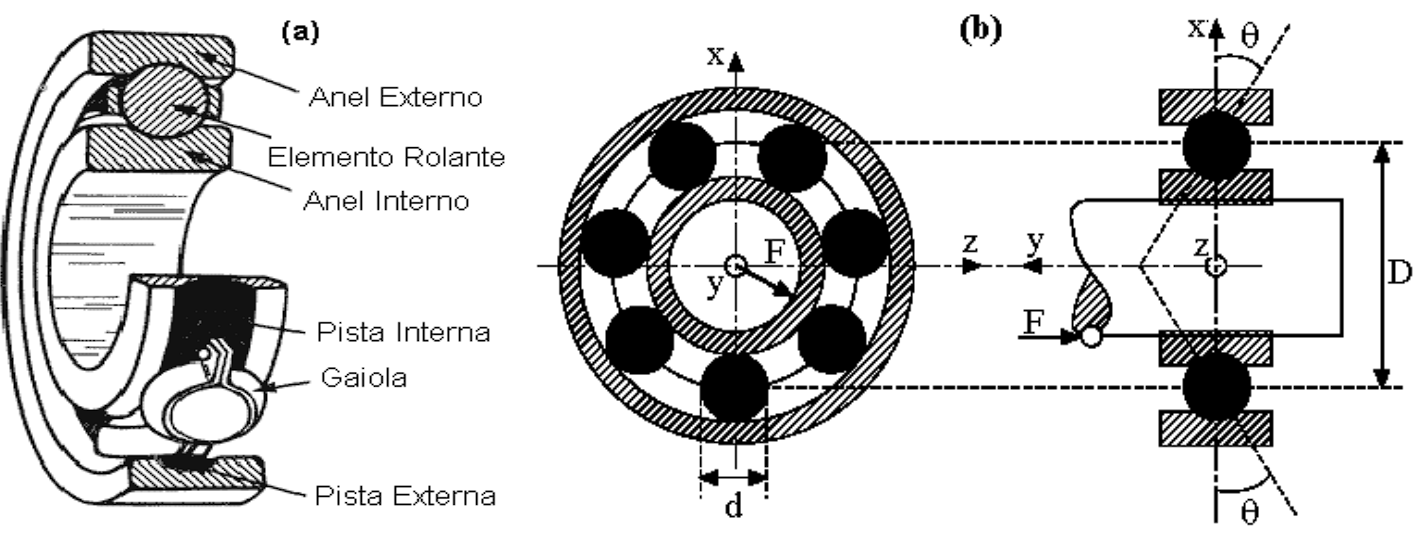
\includegraphics[width=\textwidth,height=\textheight,keepaspectratio]{Figura1}
\label{ComponentesRolamentos}
\end{figure}

Segundo a NSK (2018), rolamentos são um dos elementos de máquinas mais utilizados, visto que seu movimento rotacional torna demais movimentos mais fáceis e ajudam a reduzir fricção. Estes elementos têm dupla-função, realizando tanto a transferência de movimento, ou seja, guiando e suportando componentes que giram em relação um a outro, bem como a transmissão de forças.

Em comparação aos mancais de deslizamento, os rolamentos apresentam vantagens como: torque de partida e atrito baixos, com diferença entre torque de partida e torque de funcionamento pequenos; grande padronização internacional, facilitando sua substituição; dentre outras (NSK, 2018).

A seguir apresenta-se uma revisão sobre tipos de rolamentos, suas principais características, propriedades e tipos de falhas.

\subsection{\normalfont{\textbf{Tipos de rolamentos}}}

Os rolamentos, de forma semelhante às rodas, são componentes que podem rolar  e que servem para redução de atrito entre eles e a superfície (ABECOM, 2019). Existem distintos tipos de rolamentos, dentre os quais cita-se:

\begin{itemize}
	\item Rolamentos de rolos cilíndricos, constituídos por uma carreira de rolos em uma gaiola
	\item Rolamentos de rolos cônicos, contrítudos por pistas de anel interno e externo, cônicas e rolos cônicos
	\item Rolamentos autocompensadores, que possuem duas carreiras de esferas ou rolos com uma pista esférica comum no anel externo e duas pistas no anel interno 	
	\item Rolamentos rígidos de esfera, que são rolamentos versáteis de concepção simples e tipo não separáveis
	\item Rolamentos de esfera de contato angular, que possui pistas nos anéis interno e externo
	\item Rolamentos axiais de esferas, que são são projetados para cargas axiais não devendo ser submetidos a cargas radiais
\end{itemize}

Cada tipo de rolamento possui suas aplicações e a escolha de rolamento depende de uma série de fatores específicos, tais como a carga a ser suportada, a velocidade de funcionamento, temperatura de trabalho, folga interna, alinhamento e desalinhamento do eixo, espaço disponível, dentre outros. 

\subsection{\normalfont{\textbf{Processos de fabricação de rolamentos}}}

Nos rolamentos usualmente segrega-se o processo de fabricação em: fabricação dos anéis interno e externo; fabricação das esferas; fabricação das gaiolas e, por fim, montagem (SANTOS et al., 2017).   

As esferas, ou rolos, são feitas a partir de barras de aço cortadas em comprimentos específicos. Um processo de forjamento destes fragmentos de barra confere às peças o formato desejado, mas ainda com rebarbas. É realizado, então, o desbaste destas rebarbas. Após o processo de desbaste as esferas passam por tratamento térmico de têmpera. Por fim, é realizado o polimento. 

Os anéis interno e externo, por sua vez, são criados pelos mesmos processos, a saber: forjamento, torneamento, tratamento térmico, polimento e super-acabamento. No  primeiro processo, forjamento, os lingotes de aço são aquecidos e, através de prensagem, são formados os anéis interno e externo em cada movimento da prensa. Os processos ocorrem, portanto, simultaneamente e no mesmo equipamento. Após o forjamento, se dá o processo de torneamento. Neste, o torneamento do anel interno e externo se dá pelos mesmos passos. Primeiramente é torneada uma face lateral, a largura do anel. Em seguida, a outra face lateral é torneada. O próximo passo do processamento do anel é o torneamento do perfil da pista e largura. Simultaneamente é usinado o chanfro do anel. Em sequência ao processo de torneamento, se dá o tratamento térmico dos anéis por tempera, onde estes são aquecidos a temperaturas superiores aos \SI{800}{\celsius}, bruscamente resfriados em óleo, reaquecidos em temperaturas de \SI{150}{\celsius} e resfriados ao ar. Por fim, há o processo de acabamento onde processos abrasivos e de polimento são utilizados para atingir acabamento fino e exatidão de dimensão das peças (SANTOS et al., 2017). 

%Dar uma olhada no santos vs dos santos, arrumar essas referências

A Figura~\ref{FiguraProcessoFabricacao} demonstra o fluxo de ordenação destes processos acima descritos.
\begin{figure}[!htb]
\centering
\caption{a) Processo de fabricação dos anéis internos e externos. Retirado de SANTOS et al., 2017.}
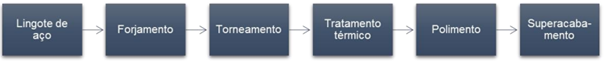
\includegraphics[width=\textwidth,height=\textheight,keepaspectratio]{Figura2}
\label{FiguraProcessoFabricacao}
\end{figure}

As gaiolas, por sua vez, são produzidas com lâminas de aço que recebem a forma de anéis planos através de estampagem, sendo, então, prensadas para receber forma ondulada a fim de manter as esferas na posição, feitos os furos para rebites e tratamento térmico da peça. (Dos Santos et al., 2017).
 
Com todas as partes produzidas é realizada, então, a montagem do rolamento. Primeiro, os anéis interno e externo são colocados concentricamente na linha de produção com as esferas preenchendo os espaços entre estes. O tamanho dos elementos rolantes se dá por calculo a partir do diâmetro da ranhura do anel interno. Estes são, então, uniformemente organizados por um divisor e uma metade da gaiola é adicionada. Em sequência outra máquina adiciona a metade restante da gaiola e finaliza-se, assim, a montagem da peça. (SANTOS et al., 2017). 

\subsection{\normalfont{\textbf{Carga e vida útil de rolamentos}}}

A vida nominal básica de um rolamento é dada na norma ISO 281:2007, que também específica os métodos de cálculo de classificação de carga dinâmica básica. Em relação a classificação de carga dinâmica básica, C, esta é utilizada para cálculos que envolvem rolamentos dinamicamente tensionados (SKF, 2019). Tal classificação expressa a carga do rolamento que resultará em uma vida nominal básica, L10, de um milhão de revoluções (SKF , 2019). O valor de C é usualmente encontrado nos catálogos referência das fabricantes.   

Para a vida nominal básica temos na ISO 281:2007 que:

\begin{equation}
	L_{10}= \left ( \frac{C}{P} \right )^{p}
	\label{eq: Vida Nominal Básica}
\end{equation}

Onde $L_{10}$ é a vida nominal básica, com 90\% de confiabilidade, expressa em milhões de revoluções; C é a classificação da carga dinâmica básica, em kN; P é a carga dinâmica equivalente do rolamento, em kN; e, por fim, p é o expoente da equação de vida, que é 3 para rolamentos de esferas e 10/3 para rolamentos de rolos (SKF, 2019).

Se a velocidade for constante, por sua vez, torna-se preferível calcular a vida útil em horas de operação (SKF, 2019). Para tanto, utiliza-se :

\begin{equation}
	L_{10h}= \frac{10^{6}}{60_{n}}L_{10}
	\label{eq: Vida Útil em Horas}
\end{equation}

Onde $L_{10h}$ é a vida nominal básica, com 90\% de confiabilidade, expressa em horas operacionais e n é a velocidade de rotação, em rotações por minuto. 
Para que se possa calcular a vida nominal básica de um rolamento usando as classificações de cargas dinâmicas básicas é necessário, entretanto, que esta seja convertida, primeiramente, em carga dinâmica equivalente do rolamento. A carga dinâmica equivalente do rolamento, P, é “definida como uma carga hipotética, com magnitude e direção constantes, que atua radialmente em rolamentos radiais e axial e centralmente em rolamentos axiais” (SKF, 2019). Esta carga hipotética teria influência na vida do rolamento igual às cargas reais que o rolamento é submetido.

Para os rolamentos híbridos, por sua vez, as mesmas vidas nominais podem ser utilizadas. Segundo a SKF, 2019, experiência e testes que a vida útil de um rolamento híbrido é maior que a vida útil de um rolamento com elementos rolantes de aço, devendo-se isto à dureza, que confere menor desgaste aos elementos rolantes, à baixa densidade, que miniza cargas internas de força centrífuga e inércia, bem como ao acabamento superficial, que otimiza os efeitos do lubrificante.

Em relação à carga mínima requerida, rolamentos que operem em alta velocidade e/ou estejam sujeitos a acelerações bruscas, forças de inércia dos elementos rolamentos e atrito do lubrificante podem ser prejudiciais aos elementos rolantes e as pistas (SKF, 2019). Assim, para o adequado funcionamento os rolamentos devem estar sujeitos a uma carga mínima de 0,01C para rolamentos de esferas e 0,02C para rolamentos de rolos. 

Por fim, em determinadas aplicações as condições operacionais, tais como a magnitude, sentido das cargas, velocidades, temperaturas e lubrificação são variáveis (SKF, 2019). O cálculo de vida útil em condições operacionais variáveis não pode ser calculado antes da redução do espectro de carga e do ciclo de trabalho. Para tanto, cada nível de carga pode ser acumulado e o espectro de carga reduzido a um histograma de blocos constantes de carga (SKF, 2019).

Para o cálculo de vida útil em condições variáveis, utiliza-se:

\begin{equation}
	L_{10}= \frac{1}{ \frac{U_{1}}{L_{10 \,1}} + \frac{U_{2}}{L_{10 \,2}} + \frac{U_{3}}{L_{10 \,3}} + ...}
	\label{eq:Calculo da vida Util em condições variaveis}
\end{equation}
%\myequation{Cálculo da vida Útil em condições variaveis}

Onde $L_{10}$ é a vida nominal básica, com 90\% de confiabilidade, $L_{10 \,1}$, $L_{10 \,2}$ são as vidas nominais básicas, com 90\% de confiabilidade, em condições constantes 1, 2 e, por fim, $U_{1}$, $U_{2}$ são as frações, que devem totalizar 1, do ciclo de vida sob as condições 1, 2 etc. De acordo com SKF, 2019, em cada intervalo de trabalho a carga e condições operacionais podem apresentar valor médio constante. Assim, o número de horas ou revoluções esperadas para cada intervalo de trabalho definem a fração de vida para esta condição específica. Neste âmbito, se ${N_{1}}$ representar o número de rotações necessárias dada uma condição de carga ${P_{1}}$, e N for o número de rotações para conclusão dos ciclos de carga variável, logo a fração do ciclo ${U_{1} = N_{1} / N}$ é utilizada pela condição de carga ${P_{1}}$, a qual apresenta vida útil calculada de ${L_{10 \,1}}$ (SKF, 2019).

\subsection{\normalfont{\textbf{Falhas em rolamentos}}}

Quando há o correto manuseio dos rolamentos, usualmente estes podem ser utilizados por longos períodos de tempo antes de surgirem sinais de fadiga. Entretanto, devido a seleção incorreta do rolamento, lubrificação inadequada ou mesmo falhas de manuseio ou de condição de serviço, podem ocorrer falhas prematuras (NSK, 2014).

Ainda que a operação se dê de forma adequada, entretanto, a ação das tensões cíclicas de cisalhamento causa o aparecimento de microfissuras que, em sua maioria, surgem em pontos de pouca resistência, ou onde o material é anisotrópico  ou em pontos onde ocorrem inclusões de materiais não metálicos. Assim, com o tempo, estas microfissuras evoluem para a superfície da pista onde surgirão microtrincas que evoluem gradativamente (HARRIS, 1991; JUVINALL e MARSHEK, 1991).

Dentre as falhas mais comuns em rolamentos temos as seguintes: escamamento, descascamento, arranhadura, escorregamento, fraturas, trinca e lascamento, gaiola danificada, impressões, \textit{pitting}, desgaste, corrosão por atrito, falso brinel, deslizamento, superaquecimento, corrosão eletrolítica, oxidação e corrosão, falha na instalação e alteração na coloração.

Escamamento é o processo em que regiões com textura áspera e grosseira são formadas por separação de pequenas partes de material dos rolamentos devido a fadiga do mesmo. Dentre as possíveis causas estão: carga excessiva, falha na instalação, carga de momento elevada, contaminação por partículas ou por água, lubrificação deficiente ou folga inapropiada (NSK, 2014). A Figura~\ref{escamemento_nsk} mostra anéis internos de rolamentos com escamamento. 

\begin{figure}[H]
\centering
\caption {Anéis internos de rolamentos apresentando escamamento. Retirado de NSK, 2014.}
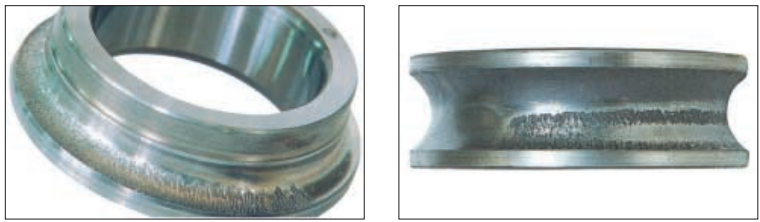
\includegraphics[width=\textwidth,height=\textheight,keepaspectratio]{escamamento_nsk}
\label{escamemento_nsk}
\end{figure}

Descascamento, por sua vez, é o processo em que a superfície da pista começa a descascar, logo sem seguida sendo percebidas ondulações. Dentre as possíveis causas para esta falha estão: excesso de carga ou manejo inadequado, montagem inadequada, precisão incorreta no eixo ou alojamento, folga insuficiente, contaminação, oxidação, lubrificação inadequada ou mesmo queda de dureza devido temperaturas altas anormais (NSK, 2014). A Figura~\ref{descascamento_nsk} mostra uma pista com descascamento.

\begin{figure}[H]
\centering
\caption {Pista de rolamento com descascamento. Retirado de NSK, 2014.}
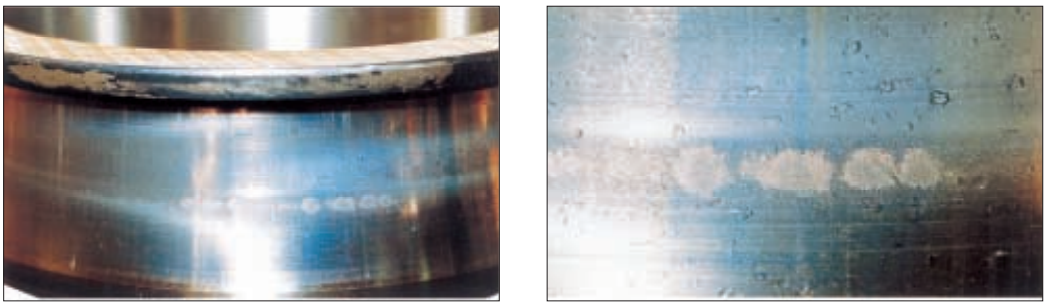
\includegraphics[width=\textwidth,height=\textheight,keepaspectratio]{descascamento_nsk}
\label{descascamento_nsk}
\end{figure}

Arranhaduras trata-se de riscos que podem ocorrer durante a montagem, arranhões em razão de objetos estranhos e duros, além de amassados superficiais devido a impactos. As causas são presença de objetos estranhos, penetração por impacto no lado descascado, quedas e choques devido manejo inadequado além de montagem desalinhada (NSK, 2014). A Figura~\ref{arranhaduras_nsk} mostra amassados e arranhaduras. 

\begin{figure}[H]
\centering
\caption {Rolamentos com amassados e arranhaduras. Retirado de NSK, 2014.}
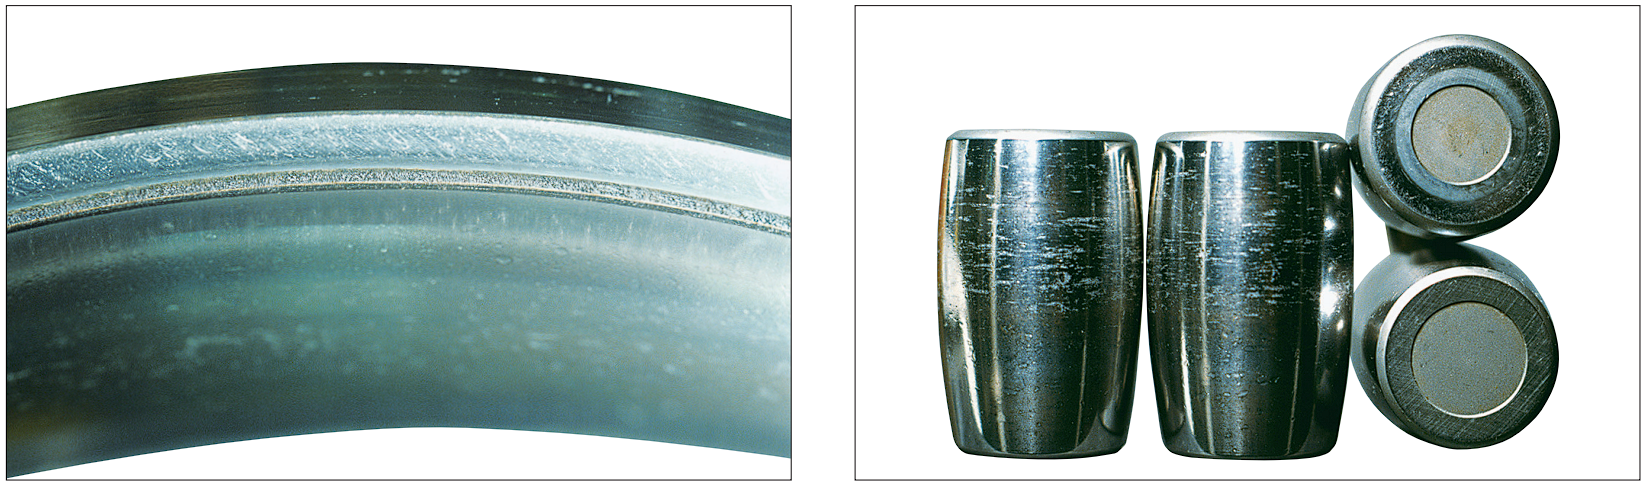
\includegraphics[width=\textwidth,height=\textheight,keepaspectratio]{arranhaduras_nsk}
\label{arranhaduras_nsk}
\end{figure}

Escorregamento refere-se ao dano causado na superficíe das pistas e elementos rolantes causados pelo rompimento do filme de lubrificação. As causas são alta velocidade e baixa carga, acelerações e desacelerações repentinas, lubrificante inadequado e entrada de água. A Figura~\ref{escorregamento_nsk} mostra um anel interno e um anel externo que sofreram escorregamento. 

\begin{figure}[H]
\centering
\caption {Aneís interno e externo com danos por escorregamento. Retirado de NSK, 2014.}
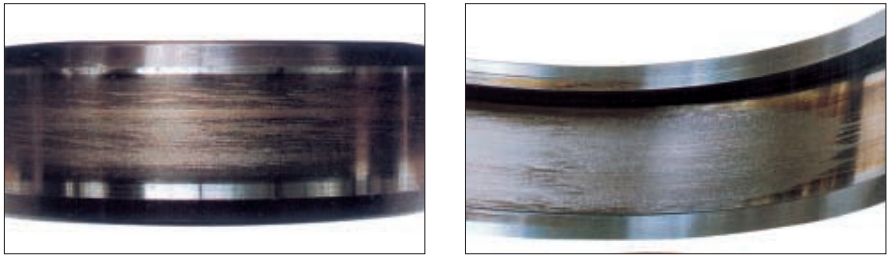
\includegraphics[width=\textwidth,height=\textheight,keepaspectratio]{escorregamento_nsk}
\label{escorregamento_nsk}
\end{figure}

Fraturas, por sua vez, referem-se à corpos rolantes partidos, anel interno ou externo partidos ou, mesmo, a gaiolas danificadas. As causas usualmente são carga anormal na gaiola por problema na instalação ou deficiência de lubrificantes, avanço do processo de escamamento ou, ainda, carga excessiva de choque e desenvolvimento de trinca de fricção. A Figura~\ref{fraturas_nsk} mostra três exemplos de anéis interno e um de anel externo com fraturas. 

\begin{figure}[H]
\centering
\caption {Anéis internos e anel externo com fraturas. Retirado de NSK, 2014.}
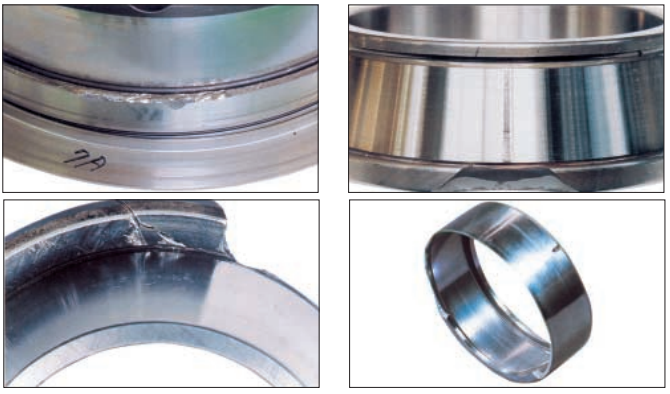
\includegraphics[width=\textwidth,height=\textheight,keepaspectratio]{fraturas_nsk}
\label{fraturas_nsk}
\end{figure}

O aparecimento de trinca e lascamento se dá quando ocorre um descascamento localizado, nisto surgem pequenas trincas ou lascamentos, dentre as possíveis causas para esta falha estão excessivas cargas de choque, excessiva interferência, formação de grandes descascamentos, formação de descascamento por atritos, encostos ou chanfros inadequados ou, ainda, manejo inadequado (NSK, 2014). A Figura~\ref{trinca_nsk} mostra rolamento com trincas e lascamentos. 

\begin{figure}[H]
\centering
\caption {Rolamento com lasca e trincas. Retirado de NSK, 2014.}
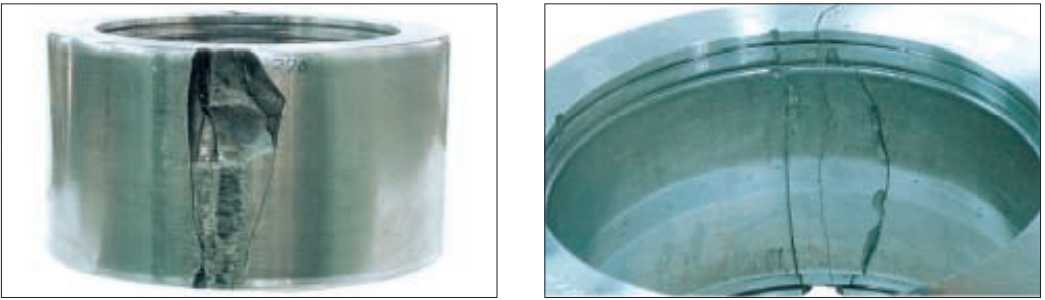
\includegraphics[width=\textwidth,height=\textheight,keepaspectratio]{trinca_nsk}
\label{trinca_nsk}
\end{figure}

Em relação a gaiola danificada, esta falha acontece quando há fratura do pilar da gaiola. Isto resulta na quebra da gaiola. As possíveis causas para esta falha são falha de instalação, carga de momento elevada, altas rotações ou excesso de variação de rotação, lubrificação inadequada, impacto com objetos estranhos, vibração excessiva ou, mesmo, aumento anormal da temperatura (NSK, 2014). A Figura~\ref{gaiola_nsk} mostra gaiolas danificadas. 

\begin{figure}[H]
\centering
\caption {Gaiolas danificadas. Retirado de NSK, 2014.}
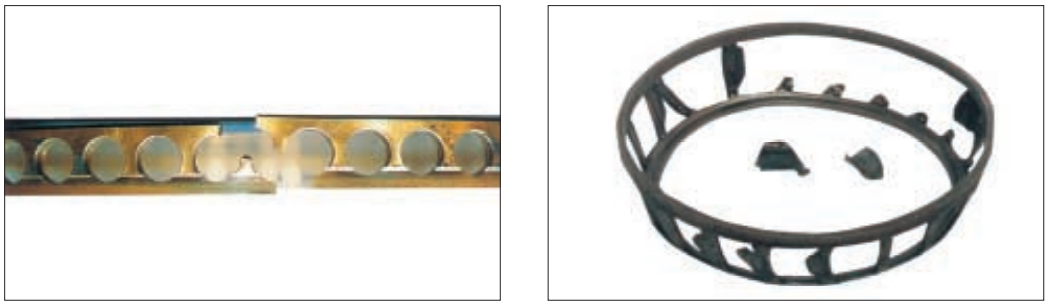
\includegraphics[width=\textwidth,height=\textheight,keepaspectratio]{gaiola_nsk}
\label{gaiola_nsk}
\end{figure}

Impressões referem-se ao ao contato de particulas com os elementos rolantes, marcando a superfície da pista e dos próprios elementos. Dentre as possíveis causas estão a contaminação por partículas, carga excerssiva ou impactos durante transporte e instalação. A Figura ~\ref{impressoes_nsk} mostra um anel interno e elementos rolantes do tipo rolos com impressões.

\begin{figure}[H]
\centering
\caption {Anel interno e rolos com impressões. Retirado de NSK, 2014.}
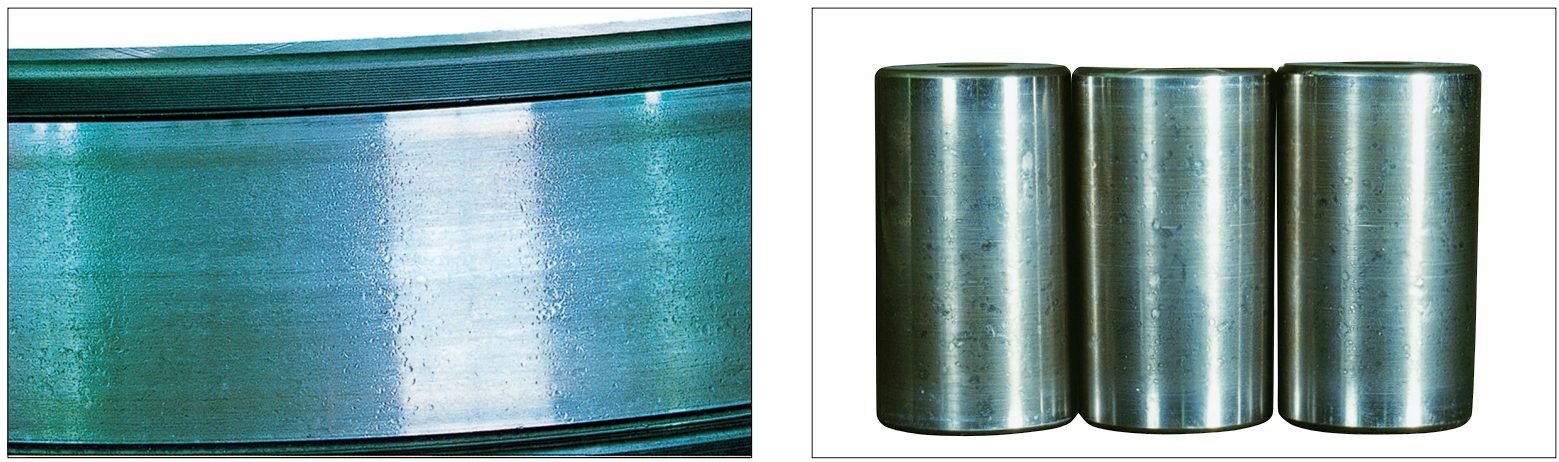
\includegraphics[width=\textwidth,height=\textheight,keepaspectratio]{impressoes_nsk}
\label{impressoes_nsk}
\end{figure}

Outra falha comum, \textit{Pitting}, ocorre quando a superfície se torna áspera e os elementos apresentam uma coloração fosca. As causas incluem lubrificação inadequada, presença de partículas estranhas, afinamento das pontas dos corpos rolantes em razão de um desalinhamento, ruptura da película lubrificante devido excesso de cargas axiais (NSK, 2014). A Figura~\ref{pitting_nsk} apresenta um anel interno e uma esfera com \textit{pitting}.

\begin{figure}[H]
\centering
\caption {Anel interno e esfera com \textit{pitting}. Retirado de NSK, 2014.}
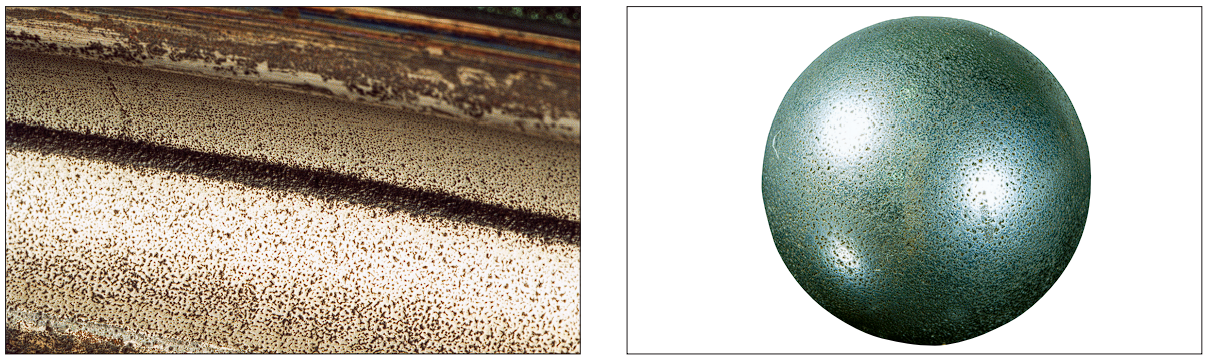
\includegraphics[width=\textwidth,height=\textheight,keepaspectratio]{pitting_nsk}
\label{pitting_nsk}
\end{figure}

Desgaste, por sua vez, é o processo em que as superfícies se desgastam e produzem uma deformação dimensional. O desgaste frequentemente acompanha rugosidade e riscos. As causas para o desgaste incluem presença de partículas estranhas no lubrificante, lubrificação inadequada e rolos afinados nas pontas (NSK, 2014). A Figura ~\ref{desgaste_nsk} mostra pistas de rolamentos com desgaste.

\begin{figure}[H]
\centering
\caption {Anel interno e externo com desgaste. Retirado de NSK, 2014.}
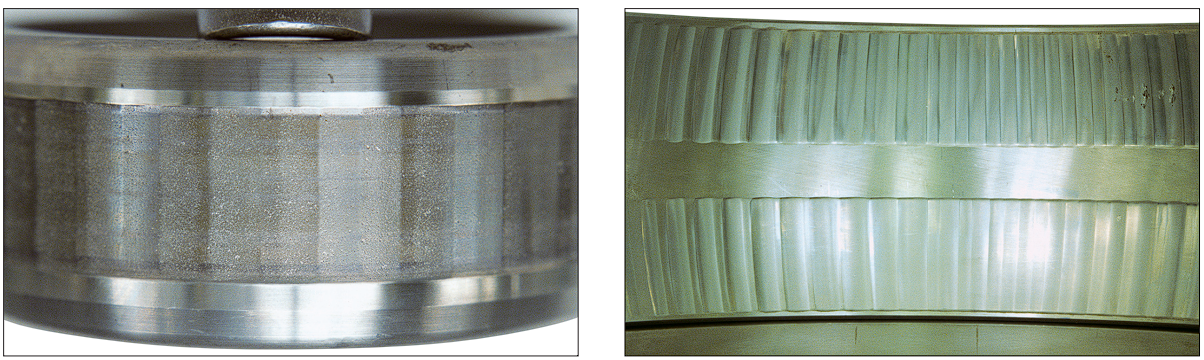
\includegraphics[width=\textwidth,height=\textheight,keepaspectratio]{desgaste_nsk}
\label{desgaste_nsk}
\end{figure}

Corrosão por contato, ou corrosão por atrito, é um tipo de desgaste por raspagem corrosiva. Há duas formas de corrosão por atrito: no primeiro, forma-se um pó de óxido sobre as superfícies de contato; no segundo, ocorre afundamentos nas pistas ao longo do passo dos corpos rolantes. As causas para estas falhas incluem ângulo de oscilação pequeno do rolamento, lubrificação insuficiente, cargas variáveis, vibração durante transporte e, ainda, interferência insuficiente (NSK, 2014). A Figura~\ref{corrosao_nsk} mostra corrosão por contato.

\begin{figure}[H]
\centering
\caption {Rolamentos com corrosão por contato. Retirado de NSK, 2014.}
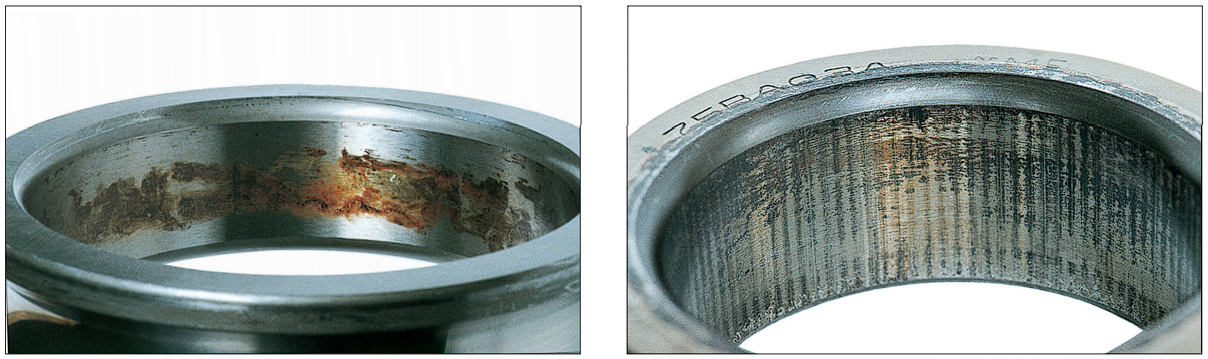
\includegraphics[width=\textwidth,height=\textheight,keepaspectratio]{corrosao_nsk}
\label{corrosao_nsk}
\end{figure}

Falso brinel refere-se ao esmagamento nas pistas e elementos rolantes por vibração ou oscilação entre os pontos de contato. Dentre as possíveis causas estão lubrificante deficiente ou pequena amplitude no movimento de oscilação (NSK, 2014). A Figura~\ref{esmagamento_nsk} mostra um anel interno e um externo com esmagamento em suas pistas.

\begin{figure}[H]
\centering
\caption {Pistas com esmagamento. Retirado de NSK, 2014.}
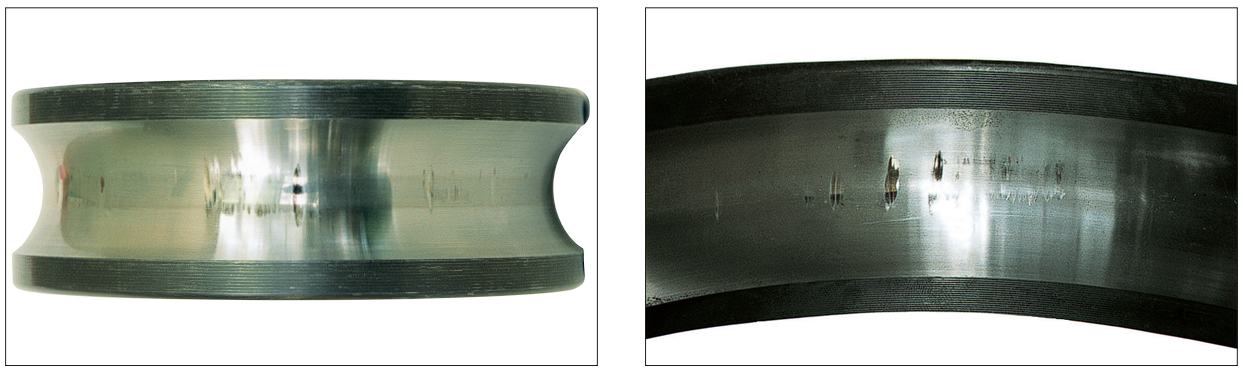
\includegraphics[width=\textwidth,height=\textheight,keepaspectratio]{esmagamento_nsk}
\label{esmagamento_nsk}
\end{figure}

Deformação de deslizamento é acompanhada de superfícies brilhantes ou de superfícies descoloridas no anel interno ou externo, também podendo ocorrer desgaste abrasivo. As causas são interferência insuficiente na seção sem brilho, bucha de montagem não fixada apropriadamente, aumento anormal de temperatura ou, ainda, cargas excessivas (NSK, 2014). A Figura~\ref{deslizamento_nsk} mostra deformação de deslizamento.

\begin{figure}[H]
\centering
\caption {Deformação de deslizamento. NSK, 2014.}
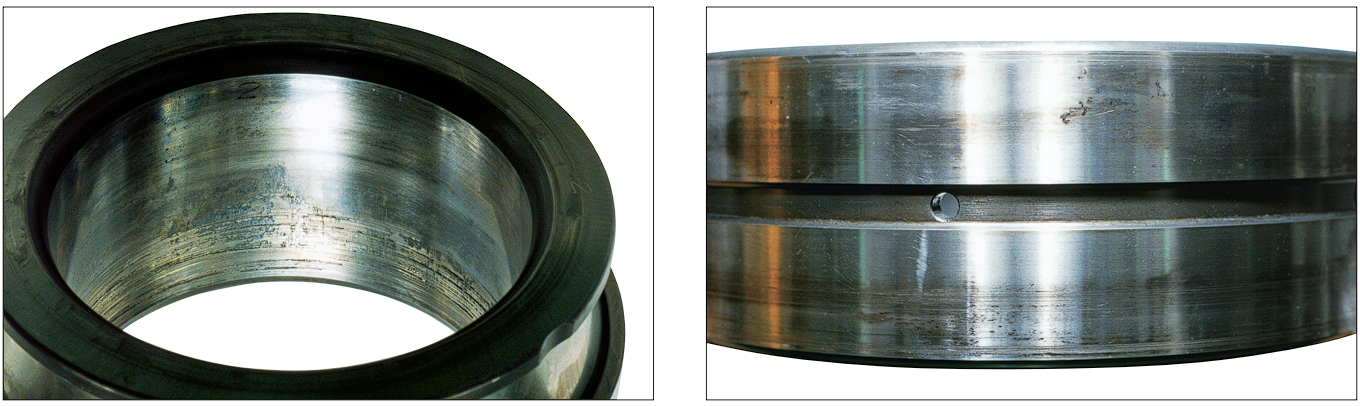
\includegraphics[width=\textwidth,height=\textheight,keepaspectratio]{deslizamento_nsk}
\label{deslizamento_nsk}
\end{figure}

Superaquecimento, por sua vez, diz respeito ao processo em que o rolamento se aquece e descolora, eventualmente travando. Dentre as possíveis causas para esta falha estão folga insuficiente no rolamento, incluindo-se folgas que diminuem em razão de deformações locais, lubrificação insuficiente ou imprópria, cargas excessivas ou ainda corpos rolantes afinados nas extremidades (NSK, 2014). A Figura~\ref{superaquecimento_nsk} mostra o dano em um rolamento que superaqueceu.

\begin{figure}[H]
\centering
\caption {Dano causado superaquecimento. Retirado de NSK, 2014.}
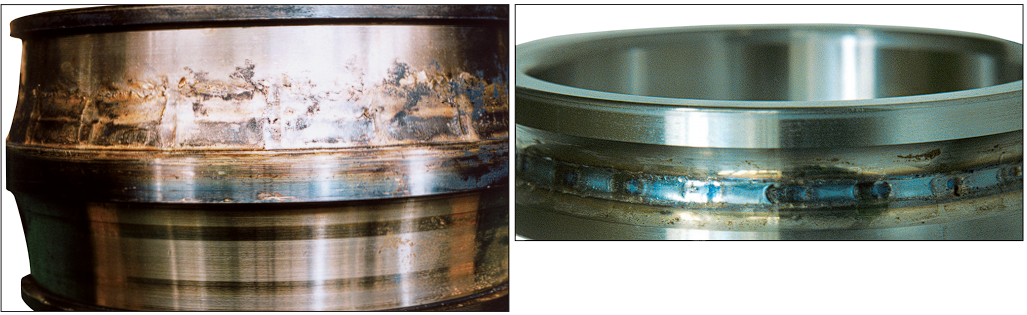
\includegraphics[width=\textwidth,height=\textheight,keepaspectratio]{superaquecimento_nsk}
\label{superaquecimento_nsk}
\end{figure}

Corrosão eletrolítica diz respeito a formação de afundamentos sobre as pistas. Estes afundamentos transformam-se gradualmente em ondulações. A causa para isto é a corrente elétrica passando através dos corpos rolantes (NSK, 2014). A Figura~\ref{corrosao_eletrolitica_nsk} mostra a corrosão eletrolítica na pista de um anel interno de um rolamento, com dano ampliado na foto para facilitação da visualização, bem como o dano em rolos. 

\begin{figure}[H]
\centering
\caption {Corrosão eletrolítica em rolamentos. Retirado de NSK, 2014.}
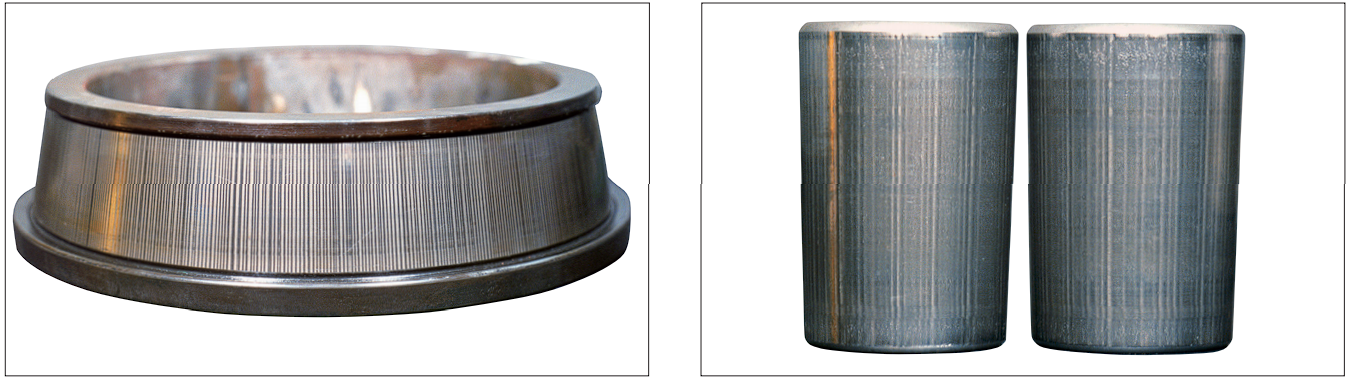
\includegraphics[width=\textwidth,height=\textheight,keepaspectratio]{corrosao_eletrolitica_nsk}
\label{corrosao_eletrolitica_nsk}
\end{figure}

Oxidação e corrosão é uma falha que ocorre quando a superfície se torna parcial ou totalmente oxidada, e ocasionalmente óxido também surge ao longo das linhas do passo dos elementos rolantes. Causas para esta falha incluem condições inadequadas de armazenamento, embalagem inadequada, óleo protetivo insuficiente, penetração de água ou ácido, dentre outros elementos, ou, ainda, manuseio inadequado (NSK, 2014). A Figura~\ref{oxidacao_nsk} mostra um rolamento oxidado e corroído.

\begin{figure}[H]
\centering
\caption {Rolamentos com oxidações e corrosões. Retirado de NSK, 2014.}
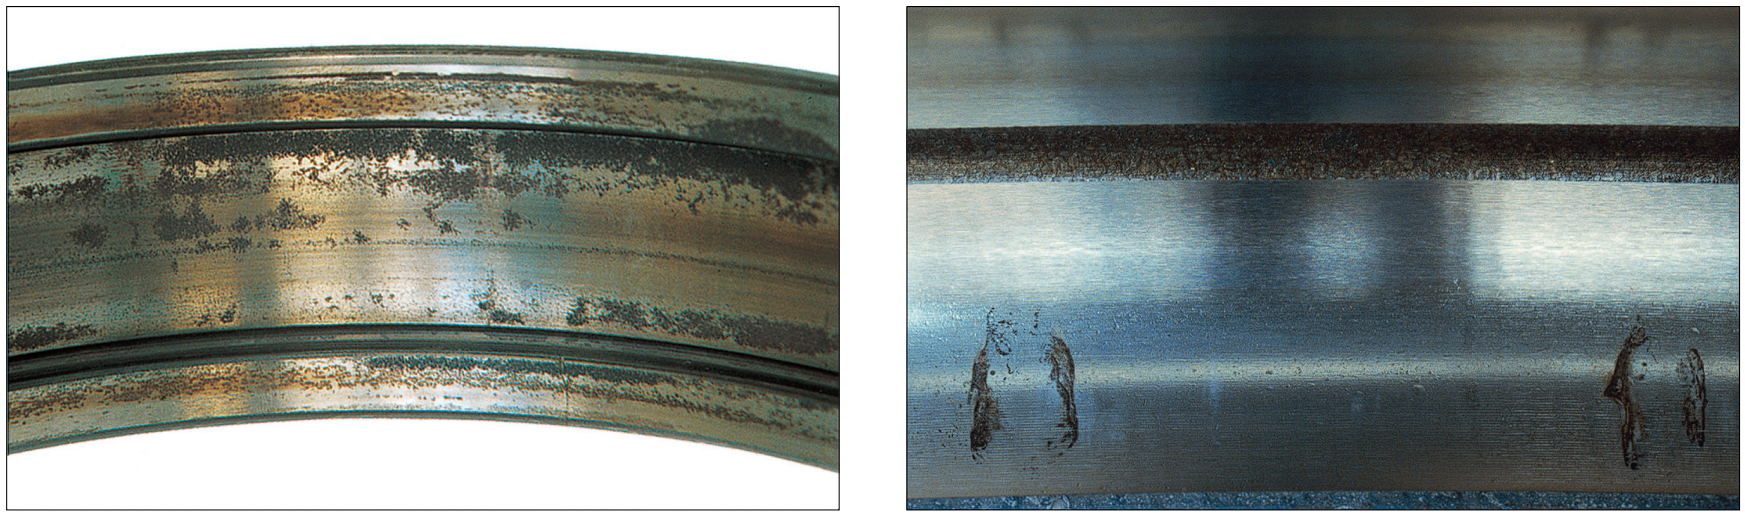
\includegraphics[width=\textwidth,height=\textheight,keepaspectratio]{oxidacao_nsk}
\label{oxidacao_nsk}
\end{figure}

Falhas na instalação têm como suas principais decorrências longo riscos na superfície das pistas ou dos elementos rolantes. As causas mais comuns são inclinação dos anéis ou impactos durante instalação ou remoção. A Figura~\ref{falha_instalacao_nsk} mostra um anel interno e externo com riscos decorrentes de falha de instalação.

\begin{figure}[H]
\centering
\caption {Rolamentos com falhas de instalação. Retirado de NSK, 2014.}
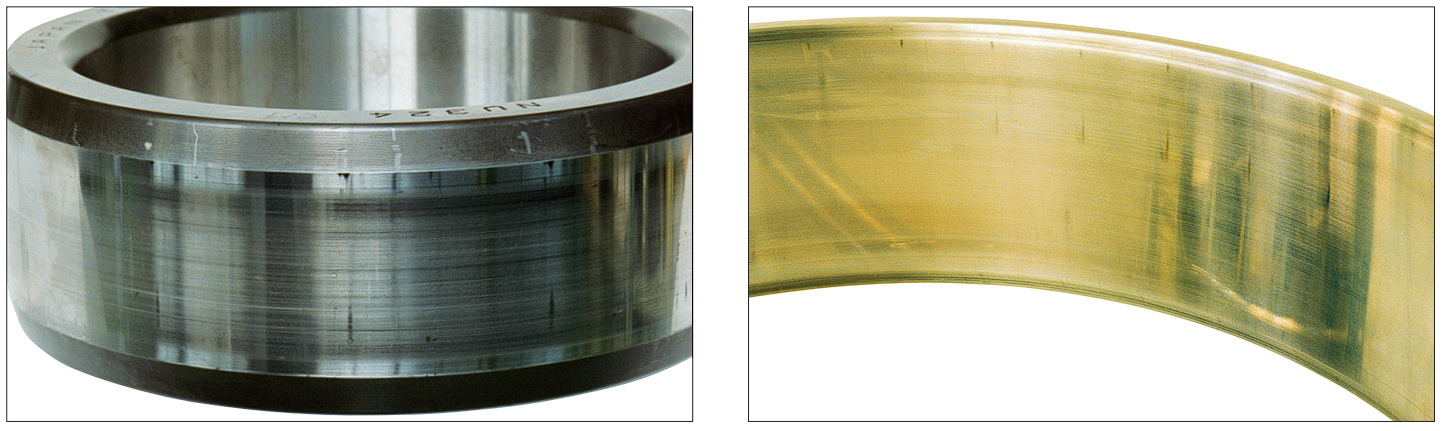
\includegraphics[width=\textwidth,height=\textheight,keepaspectratio]{falha_instalacao_nsk}
\label{falha_instalacao_nsk}
\end{figure}

Por fim, manchas e descoloração demonstram superfícies sem brilho, a superfície está fosca, rugosa ou eventualmente deformada, também estando coberta de pequenas depressões. As causas são infiltração de substância estranha ou mesmo lubrificação insuficiente (NSK, 2014). A Figura~\ref{manchas_nsk} mostra manchas e descoloração em rolamentos.

\begin{figure}[H]
\centering
\caption {Manchas e descoloração em rolamentos. Retirado de NSK, 2014.}
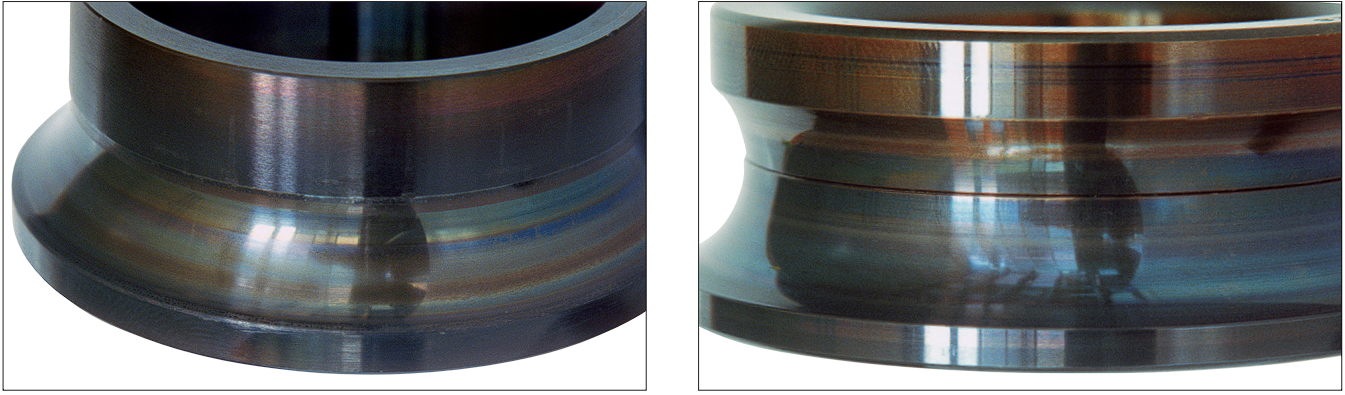
\includegraphics[width=\textwidth,height=\textheight,keepaspectratio]{manchas_nsk}
\label{manchas_nsk}
\end{figure}

Ao ocorrem danos em rolamentos, verifica-se que ocorre o contato entre a superfície defeituosa de um elemento rolante e outra superfície sem defeito. Isto gera um choque entre estes elementos, o que causa um impulso que promove uma excitação tanto na máquina, quanto no rolamento. As causas para isto são variadas.

\subsection{\normalfont{\textbf{Principais causas de defeitos em rolamentos}}}

Santander, 2014, fornece uma lista de danos primários que dão origem à danos secundários que, por sua vez, induzem falhas nos rolamentos. A Figura~\ref{falhas_comuns_rolamentos} apresenta as causas mais comuns para aparecimento de falhas em rolamentos. 

\begin{figure}[H]
\centering
\caption {Causas de defeitos em rolamentos. Retirado de NSK, 2014.}
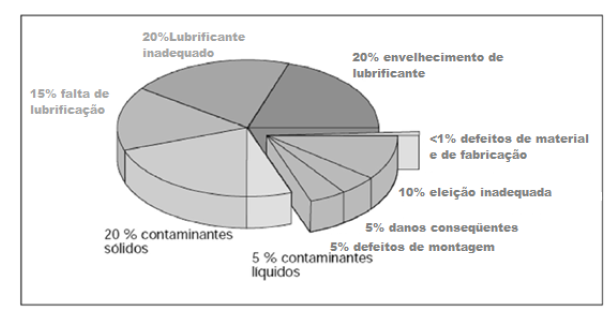
\includegraphics[width=\textwidth,height=\textheight,keepaspectratio]{falhas_comuns_rolamentos}
\label{falhas_comuns_rolamentos}
\end{figure}

Para detecção de falhas pode-se utilizar análise de vibrações, uma vez que os defeitos nos componentes dos rolamentos apresentam frequências características que podem ser calculadas a partir das especificações do rolamento. 

\newpage
\section{\normalfont{\textbf{Análise de vibrações}}}

Para que se possa abordar as técnicas de manutenção preditiva baseada em análise de vibrações faz-se necessário, primeiramente, um breve entendimento relativo ao fenômeno das vibrações mecânicas. 

Segundo Rao, 2008, a maior parte das atividades humanas envolve vibração, sendo este um fenômeno que acontece constantemente na natureza e no cotidiano. Nepomuceno, 1989, afirma que as vibrações mecânicas são fenômenos observados quando uma partícula realiza um movimento entorno uma posição de equilíbrio. Assim, quando há mudança de energia cinética para energia potencial e vice-versa, ocorre a vibração. 

Quando um corpo oscila em períodos determinados ao redor de uma posição de equilíbrio, caracteriza-se este movimento como Movimento Harmônico, forma mais simples que a vibração pode se apresentar (HOLANDA, 2016). Holanda, 2016, apresenta como exemplo disto o movimento do pêndulo de um relógio, que oscila da máxima posição à direita até a máxima posição à esquerda, passando pelo ponto central de equilíbrio. Quando este movimento oscilatório do ponto percorre uma trajetória completa, dá-se o nome de período de oscilação.  

Ressalta-se que o tempo que a massa demora para realizar uma oscilação, ou movimento harmônico simples, é chamado de período. Uma oscilação por segundo, ou um ciclo por segundo, CPS, constitui uma medida de frequência denominada Hertz (NEPOMUCENO, 1989). 

%Em relação ao movimento harmônico simples, ou oscilação, Nepomuceno, 1989, afirma que nos casos práticos, 

%\begin{citacao}
%Nos casos práticos, existem inúmeros osciladores mecânicos que são dispositivos que dão origem a oscilações simples, principalmente às amplitudes pequenas ou então fornecem combinações de oscilações. É importante observar que todo e qualquer sistema que obedeça a Lei de Hooke é apto a oferecer tal tipo de vibrações. (Nepomuceno, 1989, p.233)
%\end{citacao}

Para que se mensure os níveis de vibração, utiliza-se parâmetros expressos em termos de deslocamento, velocidade e aceleração (Holanda, 2016). Segundo Kardec e Nascif, 2009 \textit{apud} Holanda, 2016 todos os três parâmetros representam “o quanto o equipamento está vibrando”. 

Além disso, estes parâmetros possuem amplitude, frequência e fase. A amplitude, A, se relaciona com a quantidade de energia contida no sinal vibratório, ou seja, a severidade do movimento, sendo medida em milímetros (mm). Pode ser medida em forma de deslocamento, velocidade e aceleração. A frequência, f, conforme anteriormente mencionado, é representada em Hertz e indica o número de vezes em que ocorre um ciclo completo de movimento. Já a fase, $\upphi$, representa “o ângulo inicial do argumento da função senoidal que descreve o movimento harmônico” (HOLANDA, 2016, p. 22).

Já em relação às formas de mensuração, o Deslocamento é medido em micrometros (\SI{}{\micro\metre}). De acordo com Holanda, 2016, o deslocamento pode ser medido pelo nível de distanciamento do ponto relativo à sua posição de repouso, sendo a unidade mais intuitiva para a mensuração da vibração, visto que é aquuela que mais se assemelha à ideia de oscilação em torno de um ponto. O deslocamento é recomendado para medições abaixo de 10Hz (HOLANDA, 2016). A e abaixo representa o deslocamento, x:

\begin{equation}
	x = A \,sen (\omega t + \upphi)
	\label{eq:Equação de deslocamento}
\end{equation}

A velocidade, por sua vez, é medida em milímetros por segundo ($mm/s$). A velocidade é a derivada primeira do deslocamento. O deslocamento implica na existência de uma velocidade que, por sua vez, pode ser variável. A função de velocidade, v, é dada pela equação~\ref{eq:Equação de Velocidade}

\begin{equation}
	v = A\omega \,cos (\omega t + \upphi)
	\label{eq:Equação de Velocidade}
\end{equation}

Holanda, 2016, p.21 afirma que a velocidade de vibração é parâmetro “menos representativo para componentes tanto de baixa como de alta frequência, sendo o parâmetro normalmente escolhido para avaliação da severidade de vibração entre 10 Hz e 1000 Hz”.

A aceleração, por sua vez, é medida em metros por segundo ao quadrado ($m/s^{2}$). Com velocidade variável, implica-se a existência de uma aceleração no movimento. A equação que representa a aceleração, a, é:

\begin{equation}
	a = -A^{2} \omega \,sen (\omega t + \upphi)
	\label{eq: Equação de Aceleração}
\end{equation}

Limitando-se o escopo de abrangência, este fenômeno das vibrações, na engenharia, é um item de alta relevância para estudo visto que os efeitos das vibrações podem ser nocivos, ou mesmo catastróficos, ao se considerar maquinário industrial. 

Fatores como desgaste precoce de elementos mecânicos e falhas por fadiga causadas por movimentos cíclicos podem ser mensurados ao monitorar a assinatura vibracional dos componentes de máquina. A partir disto são aplicadas, então, técnicas específicas que permitam a adequada mensuração do estado dos componentes. 

\subsection{\normalfont{\textbf{Frequências características de defeitos e detecção de falhas em rolamentos}}}
\label{secao:frequenciasCaracteristicas}

De acordo com Ponci e Cunha, 2005, as frequências características de defeitos dos rolamentos são assíncronas, ou seja, estas não se dão em múltiplos inteiros da velocidade de rotação do eixo. As falhas de rolamentos geram quatro frequências características básicas, relacionadas às características e comportamento de seus componentes. 

%TO-DO: MELHORAR ESTE TRECHO

Assim, tem-se as seguintes fórmulas para o cálculo das frequências característica de defeitos nos rolamentos.

FTF (\textit{fundamental train frequency}) indica a frequência de defeito na gaiola.

\begin{equation}
	FTF = \frac{fr}{2} \left ( 1 - \frac{d}{D} \,cos \, \theta \right ) 
	\label{eq: FTF}
\end{equation}

BPFI, indica a frequência de defeito na pista interna (\textit{ball pass frenquency of the inner race})

\begin{equation}
	BPFI = \frac{N}{2}f_{r} \left ( 1 + \frac{d}{D} \,cos \, \theta \right ) 
	\label{eq: BPFI}
\end{equation}

BPFO se trata do indicativo da frequência de defeito na pista externa (\textit{ball pass frequency of the outer race})

\begin{equation}
	BPFO = \frac{N}{2}f_{r} \left ( 1 - \frac{d}{D} \,cos \, \theta \right )
	\label{eq: BPFO}
\end{equation}

BSF, por sua vez, é o indicativo da frequência de defeito do elemento rolante (\textit{ball spin frequency}).

\begin{equation}
	BSF = \frac{D}{2d}f_{r} \Bigg[  1 - \left ( \frac{d}{D} \,cos \, \theta \right ) ^{2}  \Bigg]
	\label{eq: BSF}
\end{equation}

Onde, nestas fórmulas, temos $f_{r}$, que é a subtração da frequência de rotação da pista interna pela frequência de rotação da pista externa; $D$ é diâmetro primitivo, calculado a partir da soma do diâmetro externo pelo diâmetro interno e divisão do resultado por dois; $d$ é o diâmetro dos elementos rolantes; $N$ é o número de elementos rolantes; e, por fim, $\theta$ é o ângulo de contato.

Logo, a partir destas frequências características de defeito e das especificações dos rolamentos e de suas propriedades de trabalho - número de elementos rolantes, diâmetros, ângulo de contato e velocidade de rotação -, os componentes podem ser monitorados quanto ao surgimento de falhas.  

\subsection{\normalfont{\textbf{Detecção de falhas em rolamentos por análise de vibração}}}

Abordados os conceitos  fundamentais relativos as vibrações mecânicas e as frequências que caracterizam falhas em rolamentos, faz-se necessário entender como as vibrações podem ser medidas e analisadas sob a ótica do interesse tecnológico na manutenção preditiva. 

Nepomuceno, 1989 afirma que a medida e monitoramento da vibração é uma das atividades de manutenção preditiva que apresenta melhores resultados. Mesquita et. al, 2002, afirmam que análise destas vibrações pode se dar nos domínios dotempo, da frequência e no domínio conjunto tempo-frequência.

Segundo Almeida, 2013, em relação aos rolamentos, com o surgimento de falhas são provocados impulsos através dos choques entre estas e os elementos do rolamento. Isto excita ressonâncias tanto no rolamento quanto na máquina, dadas pelas frequências características de defeitos para cada rolamento. Sabendo-se que tais frequências podem ser obtidas através das referidas características geométricas dos rolamentos, é possível que se apliquem técnicas de análise de sinais a fim de que se determine a severidade do dano e o estado do rolamento.

Em relação às técnicas específicas para análise e detecção de falhas em rolamentos, dadas as características intrínsecas destes elementos, aplicam-se técnicas no domínio do tempo, no domínio da frequência e no domínio conjunto tempo-frequência. 

Em relação à análise no domínio do tempo, Segundo Spamer, 2009, p.62 \textit{apud} Holanda, 2016, p.22 a amplitude de vibração em função do tempo pode ser medida em valores de pico a pico, valor de pico e valor RMS. Meola, 2005, afirma que o valor de pico a pico sinaliza a excursão máxima da onda, medida relevante para definição de quando um elemento da máquina atinge valores críticos. 

Já o valor de pico, de acordo com Meola, 2005, indica níveis máximos de sinais transientes, sem considerar a cronologia da onda. O valor médio, por sua vez, indica o quanto o sinal está deslocado à sua referência tendo pouca relevância quanto ao monitoramento da vibração. 

O valor RMS, ou eficaz, por sua vez, é, ainda de acordo com Meola, 2005, uma das medidas mais relevantes de amplitude, já que esta quantifica a energia diretamente ligada à vibração e, portanto, é um indicador do poder destrutivo desta. O nível RMS é, por este motivo, muito utilizado como parâmetro para determinação de níveis de alerta e alarme em manutenção preditiva (MEOLA, 2005).

A relação entre os níveis de pico, o nível médio, é dada por:

\begin{equation}
	Nivel \, M\acute{e}dio = \frac{1}{T} \int_{0}^{T} x(t)dt
	\label{eq: Nível Médio}
\end{equation}

O nível eficaz, ou nível RMS, de um sinal harmônico é dado pela equação~\ref{eq: Nível RMS}

\begin{equation}
	Nivel \, RMS = \sqrt{ \frac{1}{T} \int_{0}^{T} x^{2}(t)dt }
	\label{eq: Nível RMS}
\end{equation}

A Figura~\ref{RelacaoSinalHarmonico} exemplifica a relação estes níveis.

\begin{figure}[!htb]
\centering
\caption {Representação dos níveis de um sinal harmônico. Retirado de Meola, 2005.}
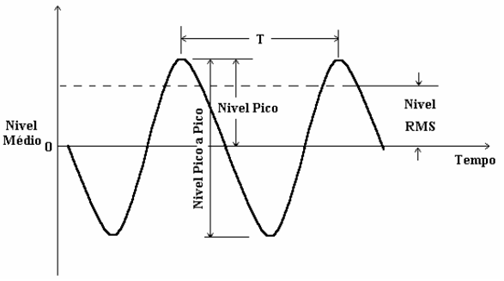
\includegraphics[width=\textwidth,height=70mm,keepaspectratio]{Figura17}
\label{RelacaoSinalHarmonico}
\end{figure}

Ainda de acordo com Meola, 2005 \textit{apud} Tandon, 1999 os métodos mais comuns de detecção de falhas no domínio do tempo são o nível RMS e o Fator de Crista, que representa a razão entre o valor de pico e o valor RMS de aceleração. O Fator de Crista, FC, considera a variação do pico e do valor RMS. Considerando-se mancais de rolamentos, Meola afirma que a diferença entre estes é de aproximadamente 3dB, dada por:

\begin{equation}
	20log_{10} \left ( \frac{Nivel \,Pico}{Nivel \, RMS} \right )
	\label{eq: Nível de Pico vs RMS}
\end{equation}

Esta diferença aumenta progressivamente com o surgimento de defeitos, até atingir valor aproximado de 18dB quando, devido ao desgaste geral do rolamento, tal diferença volta a diminuir (MEOLA, 2005). Assim, ao retornar para aproximadamente 3dB a falha é iminente e o rolamento deverá ser trocado. 

A Figura~\ref{RelacaoPicoaPicoeRMS} demonstra esta relação entre os valores de Pico e RMS.  

\begin{figure}[!htb]
\centering
\caption {Relação entre os valores de Pico e RMS com o desgaste progressivo de rolamentos. Retirado de Meola, 2005.}
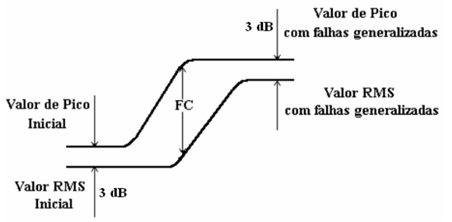
\includegraphics[width=\textwidth,height=70mm,keepaspectratio]{Figura18}
\label{RelacaoPicoaPicoeRMS}
\end{figure}	

Já a Figura~\ref{FatorCrista} demonstra o comportamento do Fator de Crista no tempo com o desgaste do rolamento.

\begin{figure}[!htb]
\centering
\caption {Fator de Crista no tempo. Retirado de Meola, 2005.}
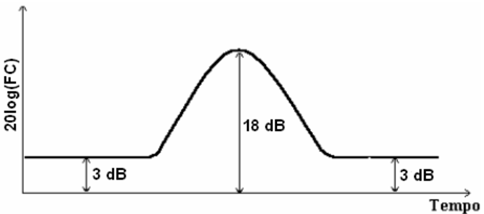
\includegraphics[width=\textwidth,height=50mm,keepaspectratio]{Figura19}
\label{FatorCrista}
\end{figure}	

Outro relevante método para detecção de falhas é a curtose. Neste, os momentos estatísticos são utilizados para descrever o comportamento de variáveis aleatórias. Segundo Mesquita et al. 2002, há diversos momentos estatísticos que podem indicar a forma da densidade de probabilidade, sendo a curtose, proposta por Dyer e Stewart, utilizada na detecção de falhas incipientes em rolamentos. O fator de Curtose trata-se do quarto momento estatístico normalizado quanto ao desvio padrão elevado a quarta potência. A curtose é descrita da seguinte forma:

\begin{equation}
	K = \frac{ \int_{-\infty}^{+\infty} (x - \overline{x})^{4}p(x)dx } {\sigma^{4}}
	\label{eq: Fator de Curtose}
\end{equation}

Ainda segundo Mesquita et al., 2002, a curtose de um rolamento em boas condições possui distribuição Gaussiana de aceleração, ao passo que rolamentos defeituosos apresentam distribuição não-Gaussiana dado o aumento no número dos altos níveis de aceleração. 

Na equação~\ref{eq: Fator de Curtose} $p(x)$ é a função de densidade de probabilidade e $\overline{x}$ o valor médio do sinal de vibração \textit{x(t)}. Segundo Mesquita et al. 2002, o fator de curtose para mancais em bom estado é próximo a três, sendo que este valor tende a aumentar conforme o rolamento se deteriora. 

É importante observar que estes métodos acima descritos, de análise de falhas no domínio do tempo, são capazes de indicar o surgimento da falha. Entretanto, tais métodos não são capazes de apontar onde se localiza tal falha. Para tanto, faz-se necessário a utilização de análise no domínio da frequência. 

Assim, tendo-se em vista que os mancais possuem frequências características de defeitos, é esperado que, ao apresentar falhas em seus componentes, tais falhas possam ser determinadas a partir das frequências por elas geradas. Desta forma, técnicas de análise espectral, tal como a transformada rápida de Fourier, podem mostrar em qual local do espectro de frequências se localiza o defeito. Mesquita et. al, 2002, entretanto, apontam para o fato de que podem ocorrer pequenos deslizamentos entre as pistas, o que pode ocasionar desvios nas frequências de defeitos em relação ao que se espera. Portanto, se recomenda que tais frequências características sejam utilizadas como referência, não como determinantes. Além disso, ainda, Mesquita et. al, 2002, atentam para o fato de que tais frequências podem ser mascaradas por outros elementos da máquina.

Dentre as técnicas de análise espectral, a mencionada transformada rápida de Fourier, conhecida pela sigla FFT, é uma das mais largamente empregadas. Entretanto, para que se obtenha resultados mais claros com a aplicação da FFT na análise espectral de rolamentos, dado o mascaramento das frequências dos por outros elementos de máquinas, fazem-se necessárias técnicas que permitam o isolamento do sinal dos rolamentos a fim de que se possa detectar os danos em sua fase inicial. 

Dentre as técnicas utilizadas para este fim, a análise de envelope é a mais largamente empregada. 

\subsection{\normalfont{\textbf{Análise de envelope do sinal}}}

Segundo Barreiro, 2010, a NASA apoiou, em 1971, um programa para investigação da detecção de defeitos em rolamentos. Neste, foram conduzidos experimentos onde se deu a comparação dos sinais de rolamentos em bom estado com o de rolamentos com danos manualmente inseridos na pista interna. Para esta comparação os dados de vibração, emissões acústicas e temperatura dos rolamentos foram capturados. A Figura~\ref{fft_sinal_barreiro} mostra a diferença entre os espectros de vibração de um rolamento em bom estado e de um rolamento com dano introduzido.

\begin{figure}[H]
\centering
\caption {Comparação de espectros de vibração de um rolamento em bom estado e de um rolamento defeituoso. O sinal acima representa o rolamento em bom estado e o sinal abaixo, o rolamento defeituoso. A faixa destacada mostra a região de dano, explicitando as diferenças entre ambos. Retirado de Barreiro, 2010.}
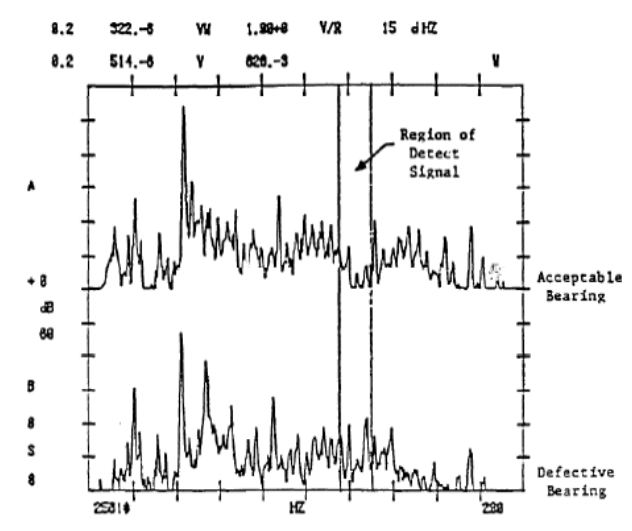
\includegraphics[width=\textwidth,height=90mm,keepaspectratio]{fft_sinal_barreiro}
\label{fft_sinal_barreiro}
\end{figure}

Dada a sútil diferença entre estes, decidiu-se conduzir maiores investigações (BARREIRO, 2010). A Figura~\ref{sinal_temporal_rolamento_barreiro} mostra o sinal do rolamento com dano introduzido visualizado, através de osciloscópio, no domínio do tempo.

\begin{figure}[H]
\centering
\caption {Sinal temporal do rolamento com dano introduzido. Retirado de Barreiro, 2010.}
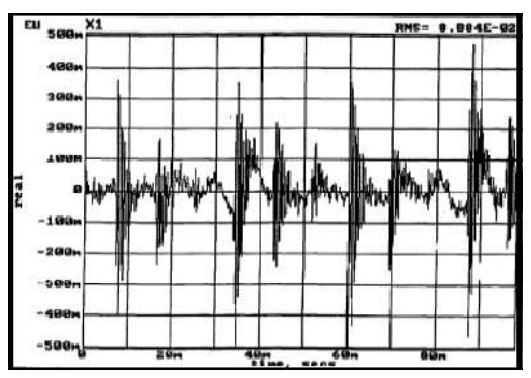
\includegraphics[width=\textwidth,height=70mm,keepaspectratio]{sinal_temporal_rolamento_barreiro}
\label{sinal_temporal_rolamento_barreiro}
\end{figure}

Com este sinal visualizado através do osciloscópio, o tempo entre os sinais de impacto foi medido e obteve-se, desta forma, a frequência de defeito na pista interna. Caso uma linha que envolvesse o sinal fosse traçada, conforme mostrado na Figura~\ref{sinal_envelope_rolamento_barreiro}, então o espectro deste novo sinal determinado por esta linha deveria mostrar a frequência do defeito. A este se dá o nome de envelope (BARREIRO, 2010). 

\begin{figure}[H]
\centering
\caption {Envelope do sinal temporal do rolamento com dano introduzido. Retirado de Barreiro, 2010.}
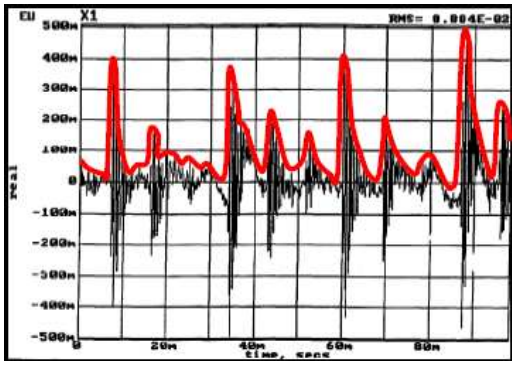
\includegraphics[width=\textwidth,height=70mm,keepaspectratio]{sinal_envelope_rolamento_barreiro}
\label{sinal_envelope_rolamento_barreiro}
\end{figure}

A Figura~\ref{espectro_do_envelope_barreiro} mostra este espectro. A seta vermelha aponta a falha, agora evidente devido sua elevada amplitude.

\begin{figure}[H]
\centering
\caption {Espectro do envelope do sinal temporal do rolamento com dano introduzido. Retirado de Barreiro, 2010.}
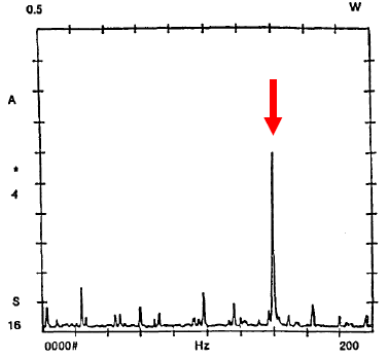
\includegraphics[width=\textwidth,height=70mm,keepaspectratio]{espectro_do_envelope_barreiro}
\label{espectro_do_envelope_barreiro}
\end{figure}

Desta forma, o trabalho aponta para a eficácia deste método na detecção de falhas incipientes em rolamentos. 

Uma vez que possibilita a detecção de falhas de rolamentos em um espectro de frequências através da comparação deste espectro com as frequências esperadas (KIM et. al, 2020). Ainda Segundo Randall, 2011 \textit{apud} Almeida, 2013, a análise de envelope da vibração tem como objetivo a troca de uma faixa mais ampla das frequências da FFT para uma faixa menor, de forma que isso permita uma análise com maior resolução. Barreiro, 2010, aponta os seguintes passos para realização da análise de envelope:

\begin{enumerate}
	\item Mudança da representação do sinal no domínio do tempo para o domínio da frequência, com utilização da FFT
	\item Filtragem do sinal através da utilização de filtro passa-faixa em torno de frequência de falha ou alteração observadas através da FFT
	\item Demodulação do sinal através da transformada de Hilbert ou da aplicação de um filtro passa-baixa, a fim de se remover do sinal os componentes de alta energia, o que possibilita maior acurácia na detecção dos defeitos do rolamento. Caso opte-se pela utilização da transformada de Hilbert, o processo de demodulação se dá através da construção de um sinal analítico complexo no domínio do tempo, onde a parte imaginária deste sinal se dá pela transformada de Hilbert da parte real.  
	\item Cálculo do espectro do sinal do envelope, onde obtém-se, em módulo, a envoltória das amplitudes obtidas após a demodulação.
	\item Utilização da FFT para transformação do domínio do tempo para o domínio da frequência, possibilitando a verificação das frequências das características de falha do mancal
\end{enumerate}

Kim afirma também que, a fim de obter uma maior acurácia do Envelope, pode ser adotada uma etapa de pré-processamento com utilização de um modelo de autoregressão do sinal, utilização de STFT e de visualização dos níveis de curtose, através da curtose espectral por janela de amostragem, para otimização da banda para o filtro passa-faixa. A Figura~\ref{envelope_kim} mostra o processo de análise de Envelope do sinal com estas etapa de pré-processamento. 

\begin{figure}[H]
\centering
\caption {Processos para . Retirado de Kim, 2020.}
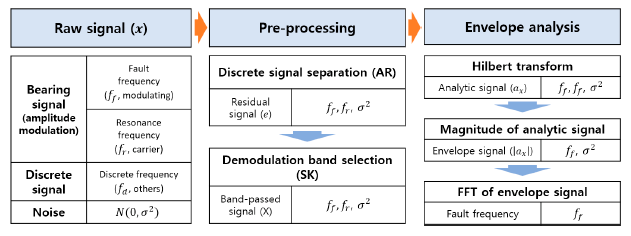
\includegraphics[width=\textwidth,height=90mm,keepaspectratio]{envelope_kim}
\label{envelope_kim}
\end{figure}

\subsection{\normalfont{\textbf{Detecção de Falhas em Mancais de Rolamentos}}}

O diagnóstico de falhas em rolamentos desempenha, como visto, um importante papel na manutenção de maquinário rotativo. Como descrito na seção~\ref{secao:frequenciasCaracteristicas}, as frequências características de defeito dos rolamentos podem ser calculadas a partir de suas propriedades geométricas e rotação ao qual estão submetidos. 

Quando um rolamento desenvolve falhas, além de apresentar tais frequências, eles geralmente passam por quatro estágios distintos de degradação (GRANEY e STARRY, 2011). 

As primeiras indicações de defeito no rolamento aparecem em frequências ultrasônicas, normalmente na região acima dos \SI{20}{\kilo{\hertz}}. Neste primeiro estágio, surgem pequenas trincas que criam ondas elásticas. A energia destas ondas ainda é baixa e a vida útil nominal esperada é de 10\% a 20\%. Desta forma, para que seja possível a detecção através de técnicas como o envelope do sinal, é necessário que o tipo de sensor utilizado tenha grande sensibilidade e seja montado o mais próximo possível da zona de carga do rolamento (GRANEY e STARRY, 2011; CBM Connect, 2021). A Figura~\ref{pitting_pista_externa} mostra um exemplo de falha neste estágio.

\begin{figure}[H]
\centering
\caption {Estágio 1}
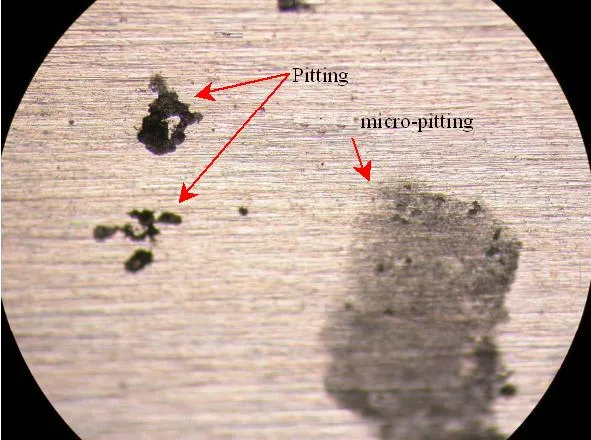
\includegraphics[width=\textwidth,height=70mm,keepaspectratio]{pitting_pista_externa}
\label{pitting_pista_externa}
\end{figure}

A Figura~\ref{estagio_1} demonstra a localização, no espectro de frequências, do sinal esperado para uma falha neste primeiro estágio, com um pico na Zona D que representa as frequências ultrassônicas.  

\begin{figure}[H]
\centering
\caption {Primeiro estágio de defeito no rolamento. Adaptado de ACOEM, 2019.}
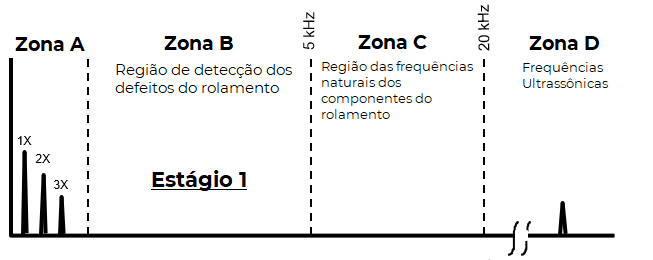
\includegraphics[width=\textwidth,height=70mm,keepaspectratio]{estagio_1}
\label{estagio_1}
\end{figure}

Já no segundo estágio de defeito no elemento rolante, a deterioração progride e a intensidade de impacto das forças também, de forma que esta torna-se suficiente para excitar as frequências naturais dos componentes do rolamento, que se encontram, usualmente, na faixa dos \SI{2}{\kilo{\hertz}} aos \SI{6}{\kilo{\hertz}} (GRANEY e STARRY, 2011; CBM Connect, 2021). Neste estágio a vida útil nominal restante é de 5\% a 10\% e o reparo em máquinas críticas deve ser agendado. A Figura ~\ref{estagio_2} mostra o aumento da amplitude na componente ultrassônica e a aparição das excitações nas frequências naturais do rolamento. 

\begin{figure}[H]
\centering
\caption {Estágio 2}
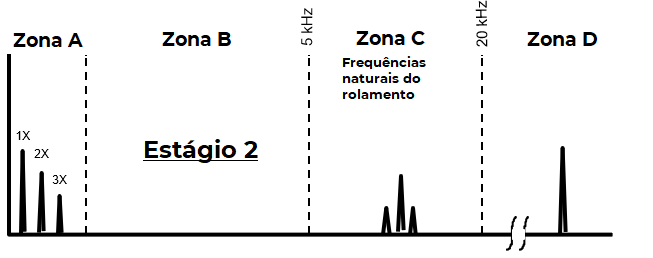
\includegraphics[width=\textwidth,height=70mm,keepaspectratio]{estagio_2}
\label{estagio_2}
\end{figure}

Já no terceiro estágio os defeitos começam a se mostrar aparentes à olho nu, sendo claramente visíveis. A deterioração progride e, nesta fase, as frequências características de defeito surgirão claramente no espectro. Uma vez que este estágio é detectado, o rolamento possui vida útil nominal restante de 1\% a 5\%, sendo necessária a parada planejada para substituição na oportunidade mais breve e seu estado monitorado com maior frequência (GRANEY e STARRY, 2011; CBM Connect, 2021). A Figura~\ref{estagio_tres_pista_externa} mostra um exemplo de rolamento com este estágio de falha em sua pista externa.

\begin{figure}[H]
\centering
\caption {Estágio 3}
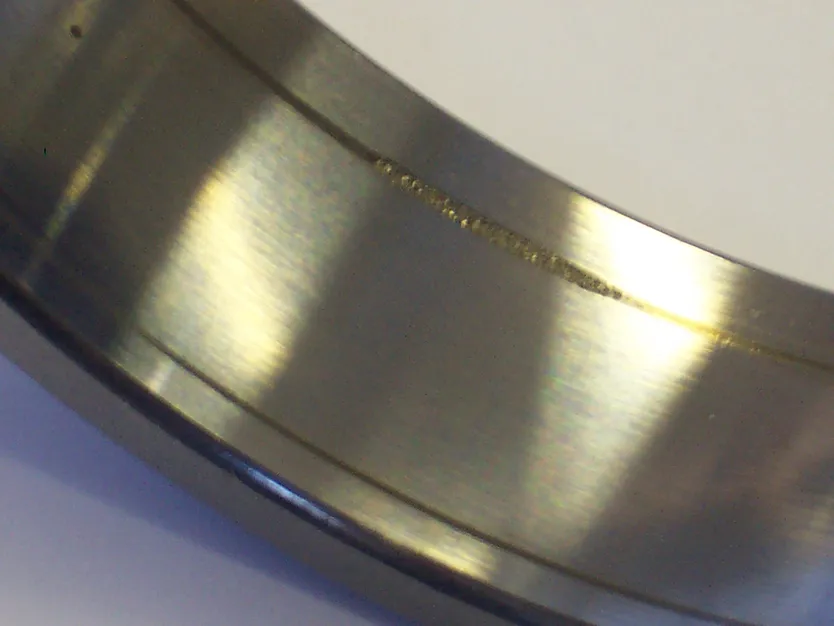
\includegraphics[width=\textwidth,height=70mm,keepaspectratio]{estagio_tres_pista_externa}
\label{estagio_tres_pista_externa}
\end{figure}

Já a Figura~\ref{estagio_3} mostra o espectro de frequências neste terceiro estágio, com aparição clara das frequências características de defeito na Zona B.

\begin{figure}[H]
\centering
\caption {Estágio 3}
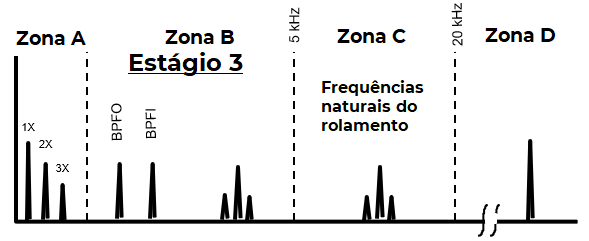
\includegraphics[width=\textwidth,height=70mm,keepaspectratio]{estagio_3}
\label{estagio_3}
\end{figure}

Por fim, o quarto estágio representa a última etapa de deterioração antes da falha total. Neste quarto estágio os métodos de detecção em alta frequência começam a falhar, pois as falhas na pista ou nos elementos rolantes começam a se arredondar e diminuem a força e intensidade dos impactos (GRANEY e STARRY, 2011; CBM Connect, 2021). Em relação às frequências de defeito, surge um ruído de fundo que máscara as frequências características, conforme visto na Figura~\ref{estagio_4}.

\begin{figure}[H]
\centering
\caption {Estágio 4}
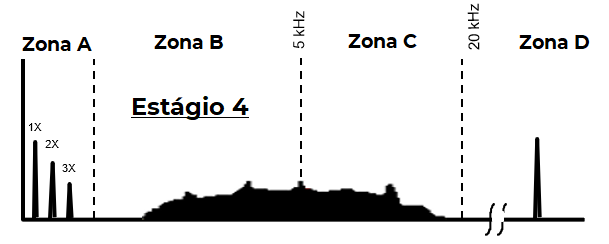
\includegraphics[width=\textwidth,height=70mm,keepaspectratio]{estagio_4}
\label{estagio_4}
\end{figure}

A partir destes quatro estágios, sob uma abordagem prática, o foco nos estágios dois e três deve ser a correta análise a fim de detectar problemas com antecedência e evitar possíveis falhas. 

Com a evolução das falhas se dará o aparecimento de frequências característiccas de defeitos, a BPFO, BPFI, BSF e FTF, que possibilitarão a determinação de onde a falha está ocorrendo. Além disto, tendo em vista que os defeitos do rolamento geram impactos, tais frequências serão frequentemente acompanhadas por diversas frequências relacionadas harmonicamente (GRANEY e STARRY, 2011). 

De um modo geral, quanto mais frequências harmônicas houver, pior será a condição do rolamento. Para detecção destas falhas, as técnicas anteriormente mencionadas, tais como a análise por meio de FFT, PSD e o método de Envelope do sinal, são empregadas. 

Para isto, entretanto, faz-se necessária a monitoração dos rolamentos com um elemento sensor, tal como filme PVDF.

\newpage
\section{\normalfont{\textbf{Fluroreto de polivinilideno}}}

O fluoreto de polivinilideno, PVDF, é um fluoropolímero termoplátisco altamente inerte produzido a partir da polimerização do monômero chamado difluoretino (kabir et al., 2017). Em 1969 um pesquisador japonês, Dr. Heiji Kawai, descobriu altíssimos níveis de atividade piezoelétrica, muito superiores a qualquer polímero natural ou sintético conhecido, no fluoreto de polivinilideno (Marutake, 1995). Desde então, o PVDF vem tendo suas aplicações estudadas. O PVDF é um polímero semicristalino de cadeia longa, proveniente da unidade CH2-CF2. Esta unidade possui um grande grande momento do dipolo elétrico, de aproximadamente 7,56 x 10-30 C.m. Como estas unidades se alinham de maneira ordenada para uma configuração \textit{head-tail} superior à 90\%, o polímero apresenta um momento líquido do dipolo elétrico incomumente alto (CHATIGNY e ROBB, 1987).

A Figura~\ref{pvdf_cadeia} mostra a estrutura molecular do PVDF.

\begin{figure}[H]
\centering
\caption {Estrutura molecular do PVDF. Retirado de Xin, 2016.}
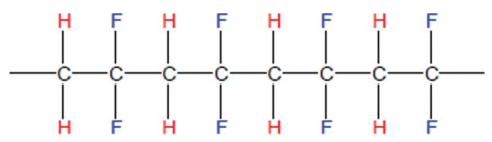
\includegraphics[width=\textwidth,height=40mm,keepaspectratio]{pvdf_cadeia}
\label{pvdf_cadeia}
\end{figure}

Decorrente desta descoberta o interesse no estudo do PVDF se dá, dentre outras caraterísticas, por suas propriedades piezo e piroelétricas. 

Piezoeletricidade é a capacidade de certos materiais, altamente polares, de alterar suas dimensões quando expostos a um campo elétrico, ou, inversamente, gerar sinal elétrico quando mecanicamente deformados (Halvorsen, 1986). A piezoeletricidade foi descoberta em 1880 pelos irmãos franceses Jacques e Pierre Curie, que a observaram em cristais de Quartzo (Manbacchi e Cobbold, 2011). Uma de suas primeiras aplicações tecnológicas foi feita por outro francês, Langevin, que desenvolveu um transmissor e receptor de quartzo para sons submarinos por volta de 1917 - o primeiro sonar (Halvorsen, 1986). Segundo Loussert et al., 2013, p.204 a piezoeletricidade se manifesta pela polarização da célula unitária com o aspecto de momento dipolar $\mu = q\times d$, onde $q$ é a carga elétrica do dípolo e $d$ é a distância entre os centroides.  

As propriedades do PVDF, incluindo a piezoeletricidade, são altamente influenciadas pelo seu grau e tipo de estrutura de cristalina. Chatigny e Robb, 1987, fazem uma revisão relacionada ao processo de fabricação de filmes PVDF para obtenção das características desejadas em cada possível estrutura cristalina deste material. Nesta, afirmam que existem três formas distintas de estrutura cristalina no PVDF. A mais comum é centrossimétrica e não polar, obtida quando o polímero é resfriado a partir de seu ponto de derretimento, chamada de fase alfa. A deformação de grãos tipo alfa, com o \textit{stretching} de filmes obtidos através de extrusão em temperaturas abaixo de \SI{80}{\celsius}, faz com que as células unitárias se alinhem em planos paralelos, criando uma fase polar chamada de fase beta. Uma terceira configuração possível é a fase gama, que, ainda que polar, é intermediária em termos de centrossimetria entre as configurações de fases alfa e beta (Chatigny e Robb, 1987).

Para obtenção de níveis significativos de atividade piezoelétrica no material, o polímero em fase beta deve ser exposto a um campo elétrico de 500kV/cm a 1000kV/cm em temperaturas de \SI{80}{\celsius} a \SI{110}{\celsius}. Este processo é chamado de \textit{poling}. O nível de atividade piezo depende do tempo de exposição a este campo elétrico, além da força do campo e da temperatura. Quando conduzido adequadamente, este processo provê orientação permanente para os dípolos no polímero (CHATIGNY e ROBB, 1987). 

Chatigny e Robb, 1987, descrevem um processo típico de preparação de um filme piezo, podendo ser resumido da seguinte forma:

\begin{enumerate}
	\item Extrusão do PVDF em filmes fase alfa; 
	\item Orientação, uniaxial ou biaxial, a \SI{80}{\celsius} e uma relação de \textit{stretch} de 4:5 para fase beta do filme;
	\item Deposição de eletrodos por algum de vários métodos;
	\item \textit{Poling} térmico a 600kV/cm a \SI{100}{\celsius}, por aproximadamente trinta minutos.
\end{enumerate}

Durante este processo, os dípolos são alinhados relativos à direção do campo de \textit{poling}. Quando o filme piezo está operando em modo eletromecânico, ele se alonga e contrai quando a polaridade dos campos se alterna. Quando operando de forma mecânico-elétrica, por sua vez, forças externas aplicadas produzem tensões de compressão e tração (CHATIGNY e ROBB, 1987). 

Os filmes PVDF são flexíveis e leves, produzidos em uma variedade de espessuras e áreas. Algumas das vantagens dos filmes PVDF incluem elevada resistência química até temperaturas elevadas , 

Devemos considerar o filme piezoelétrico como um material dinâmico que desenvolve uma carga elétrica proporcional a mudança no stress mecânico. O piezo não opera em condições estáticas devido ao rápido decaimento da carga induzida, sendo sua constante de tempo determinada pela constante dielétrica do filme e sua resistência interna. 	Uma possível analogia, fornecida por Chatigny e Robb, 1987, é a de uma esponja despejando e absorvendo um fluido, conforme uma pressão externa é aplicada e então liberada. O filme age como uma esponja liberando uma carga elétrica na frequência que a deformação tem lugar. Uma vez que a deformação cessa, nenhuma carga é transferida. 

O PVDF é um material anisotrópico.  Suas propriedades elétricas, mecânicas e eletromecânicas diferem para as excitações elétricas e mecânicas nas diferentes direções. Desta forma, para uma tabulação sistemáticas das propriedades, utilizamos três eixos identificados por números: 1, correspondente ao comprimento; 2, correspondente a altura; e, por fim, 3, correspondente a espessura (CHATIGNY e ROBB, 1987). 

Em relação a polarização do material, podemos dizer que tensões positivas são de tração, enquanto tensões negativas são compressivas. Ação elétrica positiva é causada por um aumento na polarização e vice-versa. Para os filmes piezo, o eixo de polarização é sempre a espessura, uma vez que há alinhamento do campo nesta direção. O estresse mecânico, de qualquer forma, pode ser aplicado nas três direções. 

Usualmente utiliza-se algumas constantes para caracterizar as atividades de materiais piezoativos. 

A constante de acoplamento $K$, é a habilidade de trocar energia elétrica por energia mecânica e vice-versa. O quadrado da constante $K$ é igual a energia transformada dividida pela entrada total de energia. Assim, $K312$ é igual a energia elétrica transformada causadora de tensão mecânica ao longo do eixo 1, dividida pela energia elétrica total das faces eletrificadas paralelas ao eixo 3. 

A constante de tensão piezoelétrica, $d$, expressa a razão de tensão desenvolvida ao longo de um eixo específico aplicada paralelamente a um eixo específico. 

\begin{equation}
	d_{31} = \frac{Tensao \,no \,eixo \,1}{Campo \,aplicado \,no \,eixo \,3} = \frac{m/m}{V/m} = \frac{m}{v}
	\label{eq: Constante de Tensão Piezoelétrica}
\end{equation}

%\[d_{31} = \frac{Tensao \,no \,eixo \,1}{Campo \,aplicado \,no \,eixo \,3} = \frac{m/m}{V/m} = \frac{m}{v} \]

%------- TO-DO : REVISAR ESTE TRECHO

Além disso:

\begin{equation}
	d_{31} = \frac{Carga \,por \,area \,de \,eletrodo}{Estresse \,aplicado \,no \,eixo \,1} = \frac{C/m^{2}}{N/m^{2}} = \frac{C}{N}
	\label{eq: Boa pergunta}
\end{equation}

Outra constante é a constante de estresse piezoelétrico $g$, que expressa a razão do campo elétrico ao longo de um eixo especifico pelo estresse aplicado ao mesmo ou outro eixo. A constante g também expressa a tensão ao longo de um eixo específico pela carga elétrica por área unitária de eletrodos (CHATIGNY e ROBB, 1987). Assim:

\begin{equation}
	g_{33} = \frac{Campo \,aplicado \,ao \,longo \,do \,eixo \,3}{Estresse \,aplicado \,ao \,longo ,\do \,eixo \,3} = \frac{V/m}{N/m^{2}} = \frac{Vm}{N}
	\label{eq: Constante G, expressando a razão do campo elétrico ao longo do eixo.}
\end{equation}

Também:

\begin{equation}
	g_{33} = \frac{Tensao \,no \,eixo \,3}{Carga \,por \,area \,eletronica} = \frac{m/m}{C/m^{2}} = \frac{m^{2}}{C}
	\label{eq: Contante G, expressando a tensão ao longo de um eixo específico pela carga elétrica por área unitária de eletrodos.}
\end{equation}

Também deve-se considerar a constante hidrostática piezoelétrica, $dh$, que representa a razão de carga de curto-circuito por área unitária da superfície dos eletrodos pelo estresse hidrostático aplicado igualmente ao longo dos três eixos. 

A constante piroelétrica, $p$, por sua vez, está ligada a natureza dos transdutores piezoelétricos. Estes absorvem energia térmica, aumentando assim a sua temperatura e induzindo sinais elétricos. Em filmes piezo o sinal de saída é proporcional à taxa de mudança de temperatura em vez de níveis de temperatura. A constante piroelétrica $p$, assim, relaciona a carga por unidade de área dos eletrodos pela unidade de troca de temperatura. Logo, $p = C/m^{2} K$.


\newpage
\section{\normalfont{\textbf{Sistemas de aquisição de dados}}}

Para que possa analisar os dados provenientes de sensores é necessário um sistema de aquisição de dados. França, 1997, p. 4 define sistema de aquisição de dados afirmando que este trata-se de um conjunto de elementos interrelacionados, os quais visam aquisição, análise e apresentação dos dados relativos ao processo de interesse.

Percebe-se, portanto, que um sistema de aquisição de dados é composto por diversos elementos, cada um destes com suas particularidades. França, 1997, afirma que a estrutura básica de um sistema de aquisição de dados é composta por um transdutor, condicionador, pela aquisição dos dados através de um DAQ, pela análise dos dados e, por fim, por sua apresentação. 

%Neste projeto o transdutor utilizado será o filme PVDF, cujas características.

\subsection{\normalfont{\textbf{Condicionamento de Sinal}}}
\label{sub:condicionamento}

Os sinais elétricos dos transdutores, a fim de serem aquisitados, usualmente passam por condicionamento de sinal. Este processo de condicionamento diz respeito a uma série de possíveis tratamentos que podem ser feitos em relação ao sinal elétrico, dentre as quais destacam-se a amplificação, atenuação e filtragem. 

A amplificação e atenuação tratam-se do processo de adequação das tensões elétricas obtidas por transdutores, particularmente importante em sistemas de aquisição baseados em conversores análogicos-digitais (FRANÇA, 1997). A tensão obtida pelo filme PVDF, por exemplo, usualmente encontra-se em aplicações nas quais esta precisa ser amplificada para que se adeque à faixa de conversão dos conversores analógicos-digitais. No mesmo sentido, interferências eletromagnéticas e da rede elétrica precisam ser atenuadas. 

A amplificação usualmente se dá através de um Amplificador Operacional. Este se trata de um amplificador multiestágio cujas características se almeja aproximar de um amplificador ideal: impedância de entrada infinita, impedância de saída nula, ganho de tensão infinito, resposta de frequência infinita e insensibilidade à temperatura (WENDLING, 2010). 

Já a atenuação se dá através de circuitos atenuadores, os quais são usualmente dispositivos passivos que funcionam como redes divisoras de tensão, construídas utilizando-se de resistores, os quais têm por finalidade diminuir a amplitude de um determinado sinal.

%Deslocamento de nível, por sua vez, 

Filtragem, por sua vez, diz respeito ao processo de seleção, rejeição ou equalização de uma ou várias faixas do espectro de frequências de um sinal elétrico. Ao se aquisitar o sinal de saída dos transdutores, este pode ser mais amplo que as frequências de interesse. Assim, para que se limite este sinal ao espectro desejado, utilizam-se filtros. Há diversas configurações de filtros, sendo os mais comums os filtros passa-alto, passa-baixo, passa-faixa, rejeita-faixa e passa-tudo. 

% TO-DO: melhorar acima

\subsection{\normalfont{\textbf{DAQ - Data Acquisition}}}

% TO-DO : melhorar todo este trecho

Em especial quanto ao condicionamento e aquisição de sinais, destaca-se em particular as questões de amplificação e atenuação do sinal, essenciais em sistemas baseados em conversores analógico-digitais, A/D, onde obtém-se um sinal analógico - tal qual a tensão elétrica de um sensor de filme PVDF - e este é discretizado para representação digital. 

Assim, ao lidar com sistemas baseados os conversores analógico-digitais estes estão costumeiramente disponíveis em DAQs, sigla para \textit{Data Acquisition}, que podem tomar formas desde dispotivos específicos para a aquisição de dados até microcontroladores com conversores A/D embarcados. Alguns dos princiapis aspectos relativos aos DAQs e seus conversores analógicos-digitais são: número de canais, resolução, faixa de conversão e taxa de amostragem.

De acordo com a Omega, 2021, o conversor analógico-digital trata-se de um "dispositivo eletrônico que converte sinais analógicos em um formato digital equivalente". Este dispositivo é central na grande parte dos sistemas de aquisição de dados, uma vez que é o responsável pela representação digital dos sinais analógicos de interesse. 

%Em relação a filtragem destes sinais, França, 1997, p. 7, afirma que "o espectro de frequências do sinal na saída dos transdutores pode ser muito mais amplo do que é de interesse". Neste sentido, aplicam-se filtros para atenuação de sinais indesejados.

O número de canais de um DAQ trata-se da quantidade de entradas disponíveis para aquisição de dados. As faixas de conversão, de acordo com França, 1997, p. 15, são os limites de tensão máximo e mínimo que um conversor analógico-digital está apto a quantizar.

Já a resolução, de acordo com a Omega, 2021, trata-se do "menor incremento de sinal que pode ser detectado por um sistema de aquisição de dados", em relação a uma faixa de conversão estabelecida. A resolução é expressa em bits, porcentagem ou fundo de escala. Para um DAQ com resolução de 12 bits e faixa de conversão de \SI{5}{\volt}, temos 

\begin{equation}
	\frac{\SI{5}{\volt}}{2^{12}} = \SI{1,22}{\milli\volt}
	\label{eq: Resolução de DAQ de 12 bits com faixa de conversão de 5 volts}
\end{equation}

%\[\frac{\SI{5}{\volt}}{2^{12}} = \SI{1,22}{\milli\volt} \]  

Percebe-se, portanto, que quanto maior a resolução, menores estes incrementos. 

Já a velocidade, de acordo com a Omega, 2021, trata-se de "a velocidade na qual um sistema de aquisição de dados coleta os dados. Normalmente, a velocidade é expressa em amostras por segundo". 

Para dispositivos multicanais, a taxa de amostragem é geralmente, mas não sempre, a velocidade do conversor analógico digital dividida pelo número de canais amostrados. 

Iazzetta, 2021, afirma ainda em relação as taxas de amostragem que estas são o número de vezes em que se realiza uma amostragem, por unidade de tempo. A taxa de amostragem geralmente é medida em Hertz. 

%--------- TO-DO: reescrever citação abaixo.

%\begin{citacao}
%\,[...]O números de vezes em que se realiza a amostragem em uma unidade de tempo é a taxa de amostragem, geralmente medida em Hertz. Assim, dizer que a taxa de amostragem de áudio em um CD é de 44.100 Hz, significa que a cada segundo de som são tomadas 44.100 medidas da variação de voltagem do sinal. Dessa maneira, quanto maior for a taxa de amostragem, mais precisa é a representação do sinal, porém é necessário que se realize mais medições e que se utilize mais espaço para armazenar esses valores.
%\end{citacao}

Em relação a taxa de amostragem, o teorema de Nyquist, também conhecido como teorema de amostragem de Nyquist-Shannon, afirma que é necessário uma taxa de ao menos duas vezes o valor da frequência máxima de interesse para que se possa realizar a análise desta. Esta taxa é chamada frequência de Nyquist. Caso a taxa de amostragem seja menor que a frequência de Nyquist, há ocorrência do efeito conhecido como \textit{aliasing}, onde um sinal é incorretamente reconstruído como um sinal de baixa frequência.

%https://br.omega.com/prodinfo/aquisicao-de-dados.html



\chapter{Materiais e métodos}
\label{secao:MateriaisEMetodos}
% TO-DO: MELHORAR TODA ESTA SEÇÃO

Neste capítulo são descritos os materiais empregados e métodos adotados para os experimentos, também descritos nesta seção, a fim de se investigar a viabilidade do sensor filme PVDF para fins de manutenção preditiva em rolamentos. 


\section{\normalfont{\textbf{Rolamentos autocompensadores de rolos}}}

Para a realização dos experimentos foram utilizados dois rolamentos de rolos autocompensadores da NSK, modelo 21306CD. Este modelo apresenta como principais características uma alta capacidade de carga, gaiola de aço prensado e desalinhamento permissível entre $1^{\circ}$ e $2.5^{\circ}$. Esta categoria de rolamento foi escolhida pois possibilita uma maior facilidade para inserção manual de defeitos quando comparado, por exemplo, com rolamentos de esferas blindados. A inserção manual de defeitos é uma etapa necessária para possibilitar, nos experimentos, o emprego dos métodos de análise dos sinais do rolamento defeituoso para detecção das frequências características de defeito com utilização do filme PVDF. 

As dimensões do rolamento escolhido são:

\begin{itemize}
	\item Número de elementos rolantes: 26 (13 por fileira)
	\item Diâmetro externo: 72 \si{\mm}
	\item Diâmetro interno: 30 \si{\mm}
	\item Limite de rotação: 4500 RPM lubrificado a graxa, 6000 RPM lubrificado a óleo
\end{itemize}

A Figura~\ref{Figura24} mostra um modelo de rolamento autocompensador de rolos, tal como utilizado na bancada experimental.

\begin{figure}[H]
\centering
\caption {Rolamento autocompensador de rolos. Retirado de NSK, 2018.}
\includegraphics[width=\textwidth,height=50mm,keepaspectratio]{Figura24}
\label{Figura24}
\end{figure} 

A Figura~\ref{rolamento_caixa_aberta} mostra os rolamentos já acoplado ao eixo motriz na bancada experimental, dentro de suas respectivas caixas.

\begin{figure}[H]
\centering
\caption {Rolamento autocompensador de rolos. Retirado de NSK, 2018.}
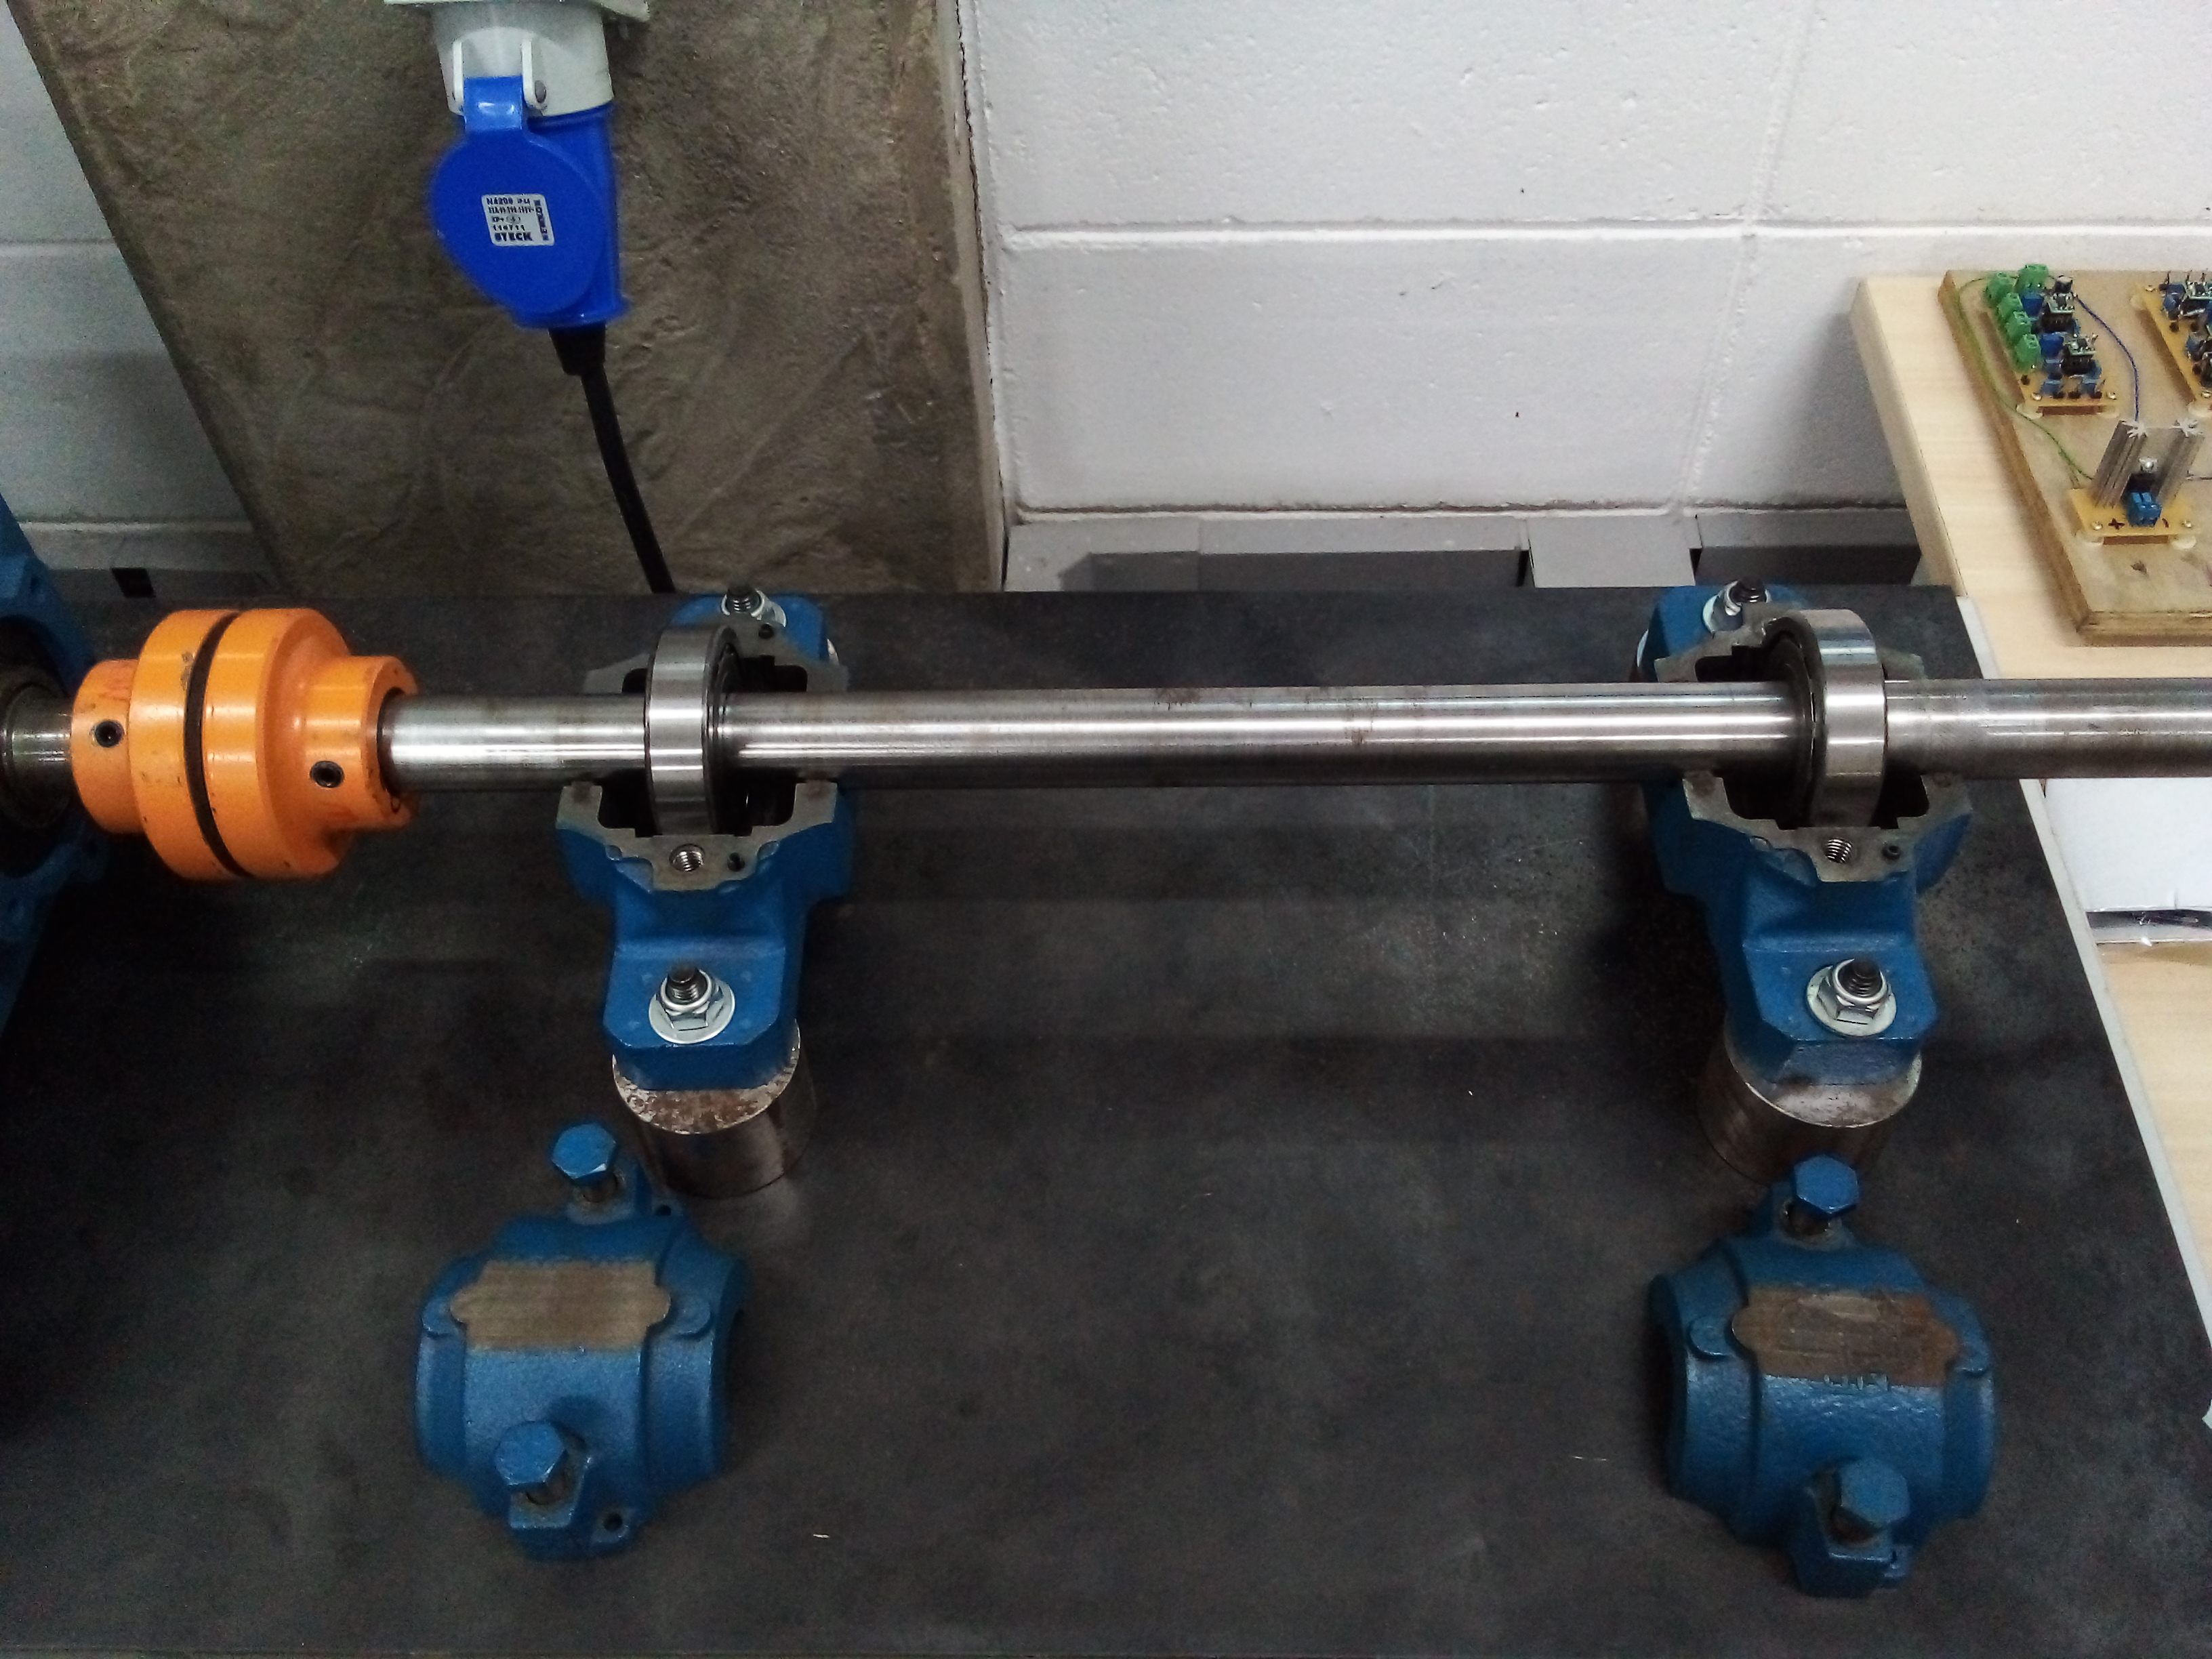
\includegraphics[width=\textwidth,height=120mm,keepaspectratio]{rolamento_caixa_aberta}
\label{rolamento_caixa_aberta}
\end{figure} 

Algumas das medidas do rolamento necessárias para o cálculo das frequências características de defeito, a saber o ângulo de contato e o diâmetro dos elementos rolantes, estão disponíveis no \textit{website} da fabricante NSK em um modelo CAD do mesmo, onde a partir deste calcularam-se os seguintes valores:

\begin{itemize}
	\item Diâmetro dos elementos rolantes: aproximadamente 10\si{\mm}
	\item Ângulo dos elementos rolantes: aproximadamente 14\textdegree
\end{itemize}

A Figura~\ref{angulo_de_contato} mostra o CAD do rolamento NSK 21306CD com vista frontal, estando com as marcações para mensuração do ângulo de contato. 

\begin{figure}[H]
\centering
\caption {Ângulo de contato calculado a partir do modelo CAD disponibilizado pela NSK. Elaborado pelo autor.}
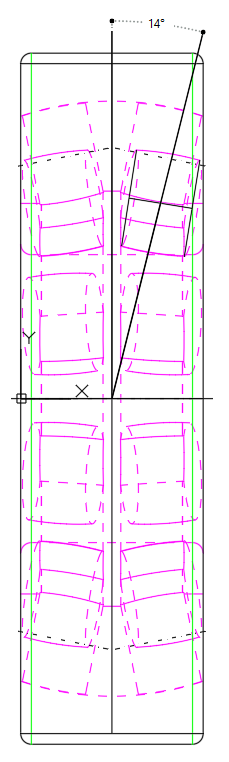
\includegraphics[width=\textwidth,height=100mm,keepaspectratio]{angulo_de_contato}
\label{angulo_de_contato}
\end{figure} 

Já a Figura~\ref{diametro_rolamento} apresenta o diâmetro do elemento rolante, calculado a partir do raio de um dos elementos rolantes visto a partir da face direita do rolamento. 

\begin{figure}[H]
\centering
\caption {Diâmetro do elemento rolante calculado a partir do modelo CAD disponibilizado pela NSK. Elaborado pelo autor.}
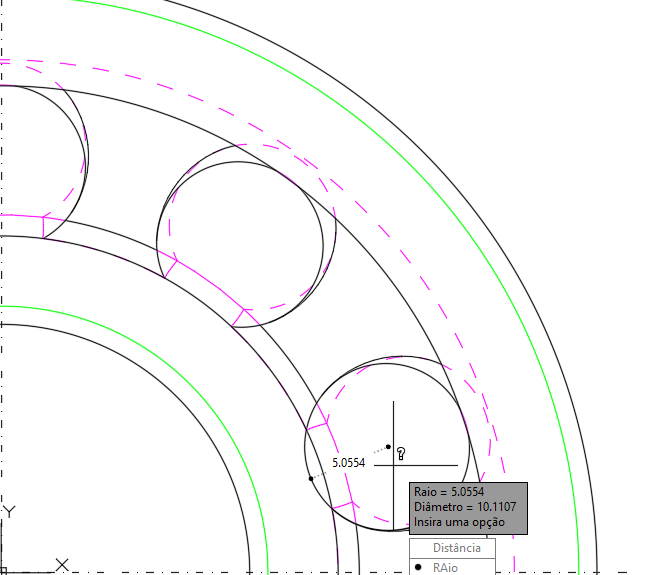
\includegraphics[width=\textwidth,height=75mm,keepaspectratio]{diametro_rolamento}
\label{diametro_rolamento}
\end{figure} 

As amostras do rolamento escolhido são novas e isentas de qualquer tipo de falha. Estas foram montadas em uma bancada experimental, construída para condução dos experimentos, onde foram registradas as suas assinaturas de vibração tanto no domínio da frequência, quanto do tempo para posterior análise. 

\section{\normalfont{\textbf{Bancada experimental}}}

O aparato experimental é composto por um motoredutor cedido pela empresa parceira WEG/Cestari, com eixo motriz usinado e ligado à mancal de rolamento de empresa parceira NSK. A bancada possui em sua base um isolador de vibrações do tipo vibra-stop. A Figura~\ref{Figura22} mostra o projeto da bancada experimental. 

\begin{figure}[H]
\centering
\caption {Projeto da bancada experimental. Elaborado pelo autor.}
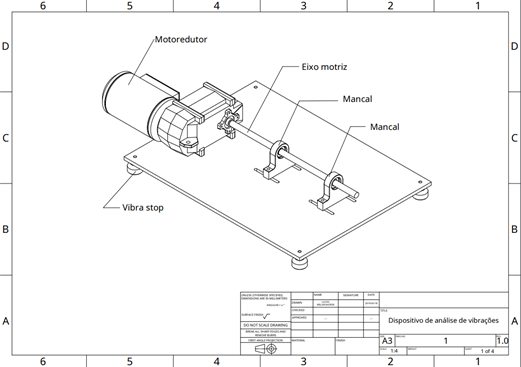
\includegraphics[width=\textwidth,height=\textheight,keepaspectratio]{Figura22}
\label{Figura22}
\end{figure}

A Figura~\ref{dispositivo_teste_visto_de_lado} mostra uma visão lateral do dispositivo que será utilizado. Os sensores com seus respectivos acoplamentos serão afixados nos mancais. 

\begin{figure}[H]
\centering
\caption {Projeto da bancada experimental visto lateralmente. Elaborado pelo autor.}
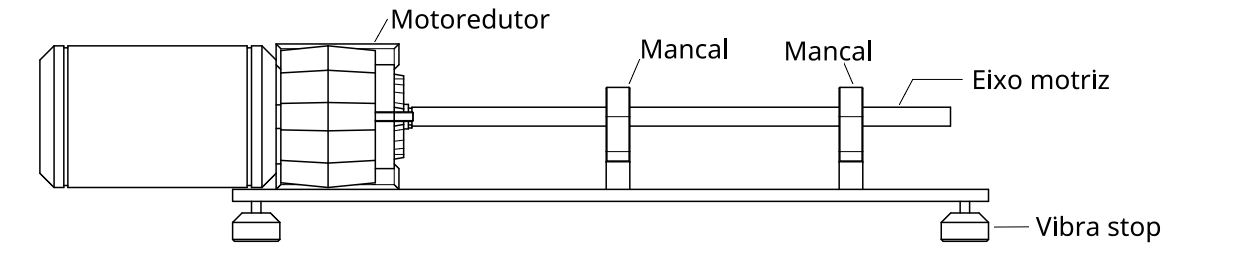
\includegraphics[width=\textwidth,height=\textheight,keepaspectratio]{dispositivo_teste_visto_de_lado}
\label{dispositivo_teste_visto_de_lado}
\end{figure}

Em relação a construção da bancada experimental, foi utilizado um torno mecânico do IFSP Câmpus Guarulhos para usinagem do eixo, e foi utilizada prensa a fim de realizar o acoplamento dos mancais de rolamentos ao eixo usinado e posteriormente este foi ligado ao motoredutor. A Figura~\ref{bancada_de_testes} mostra a bancada experimental em sua fase inicial de elaboração.

\begin{figure}[H]
\centering
\caption {Bancada experimental. Elaborado pelo autor.}
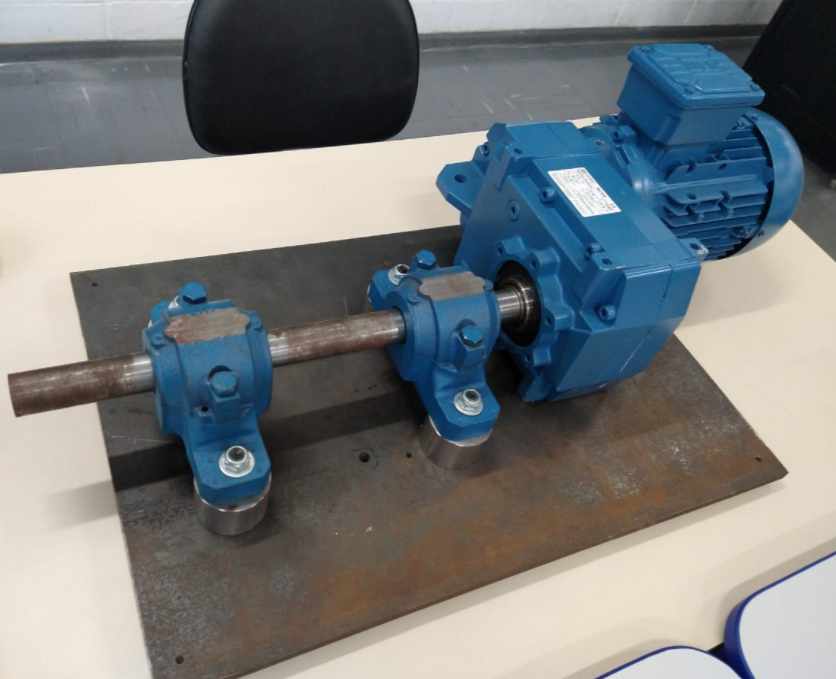
\includegraphics[width=\textwidth,height=100mm,keepaspectratio]{bancada_de_testes}
\label{bancada_de_testes}
\end{figure}

Já a Figura~\ref{bancada_completa} mostra a bancada com construção finalizada.

\begin{figure}[H]
\centering
\caption {Bancada experimental. Elaborado pelo autor.}
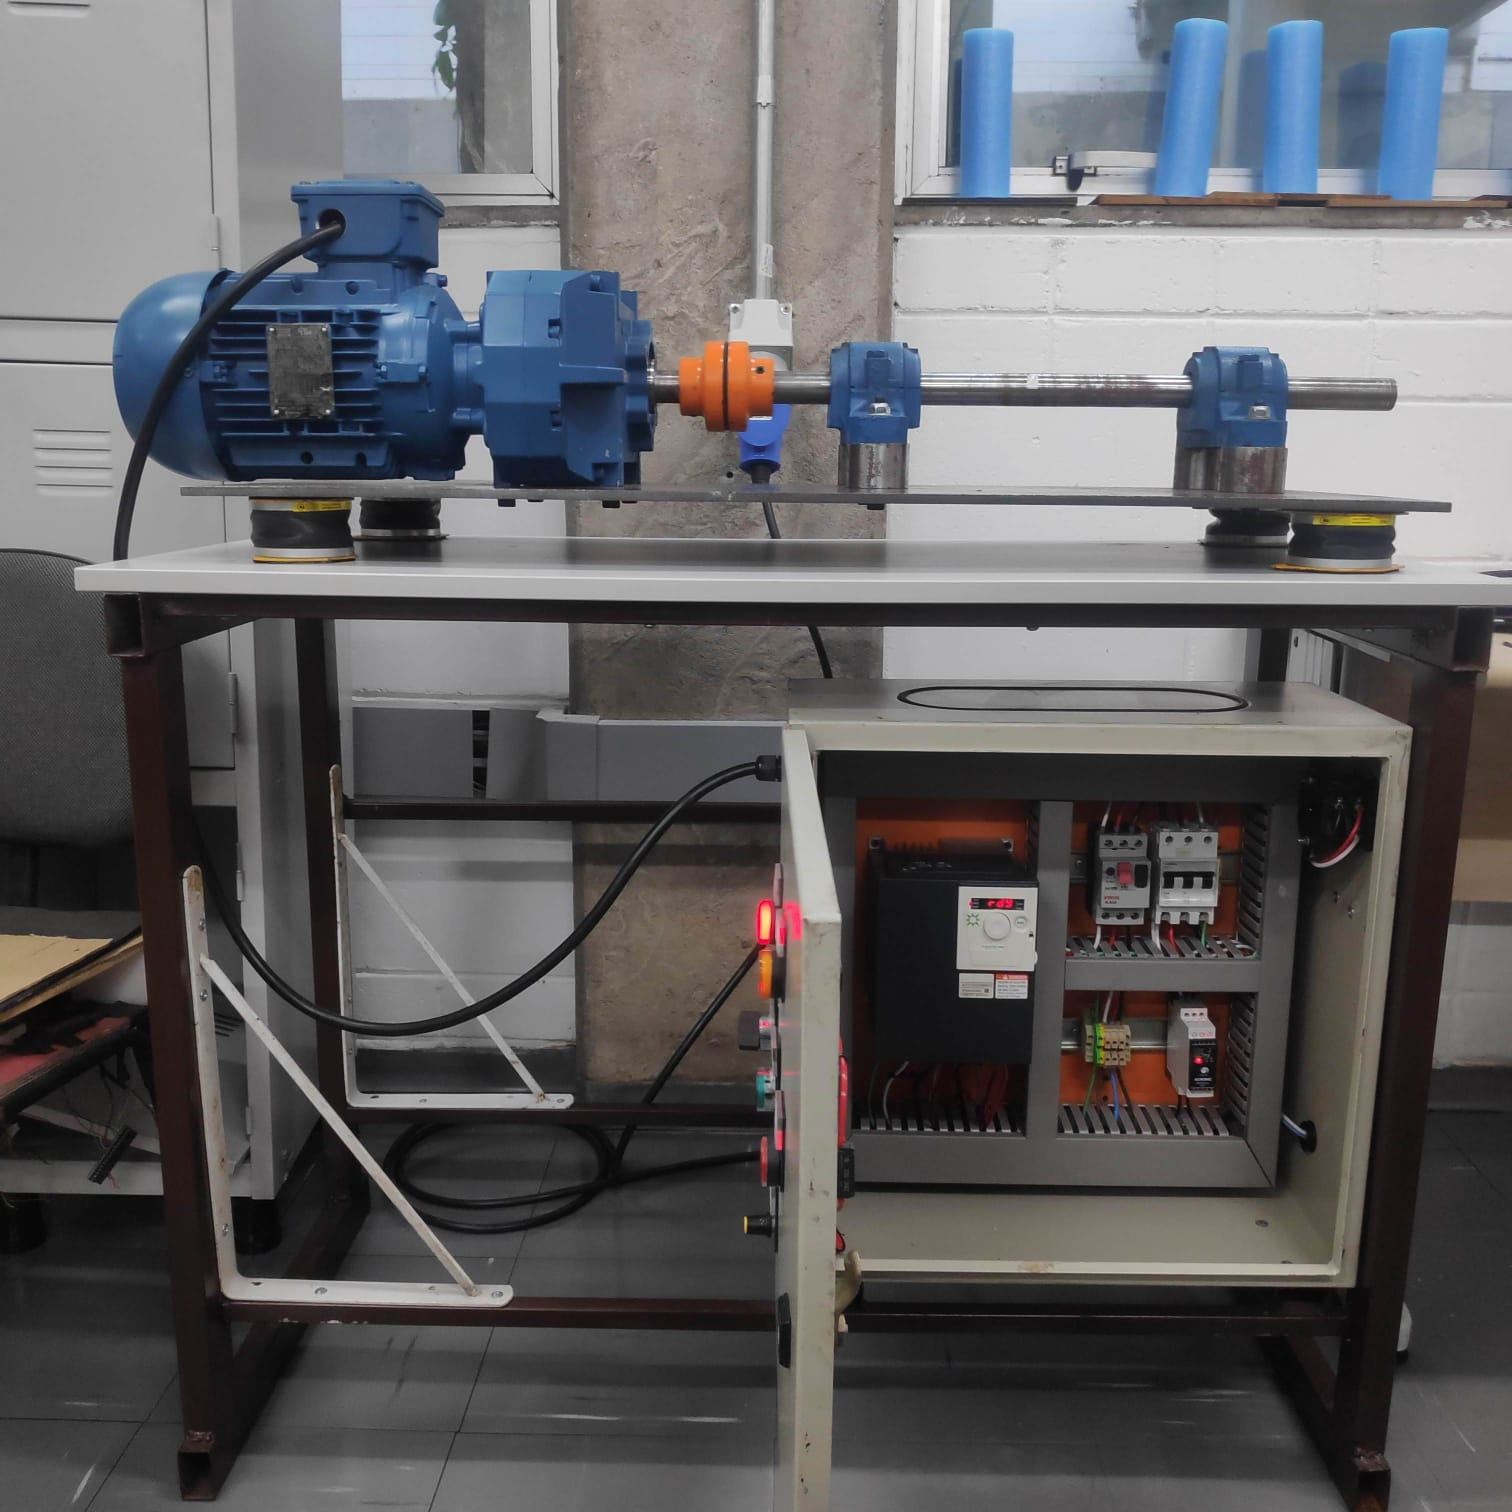
\includegraphics[width=\textwidth,height=100mm,keepaspectratio]{bancada_completa}
\label{bancada_completa}
\end{figure}

Ao projeto inicial optou-se incluir duas melhorias: dispositivos isoamortecedores, capazes de bloquear vibrações externas para a bancada, bem como um acoplamento no eixo. A Figura~\ref{isoamortecedor_bancada} mostra o isoamortecedor da marca Gerb instalado. O projeto de instalação e dimensionamento do isoamortecedor está disponível no Apêndice~\ref{secao:apendiceIsoamortecedor}. 
 
\begin{figure}[H]
\centering
\caption {Isoamortecedor Gerb. Elaborado pelo autor.}
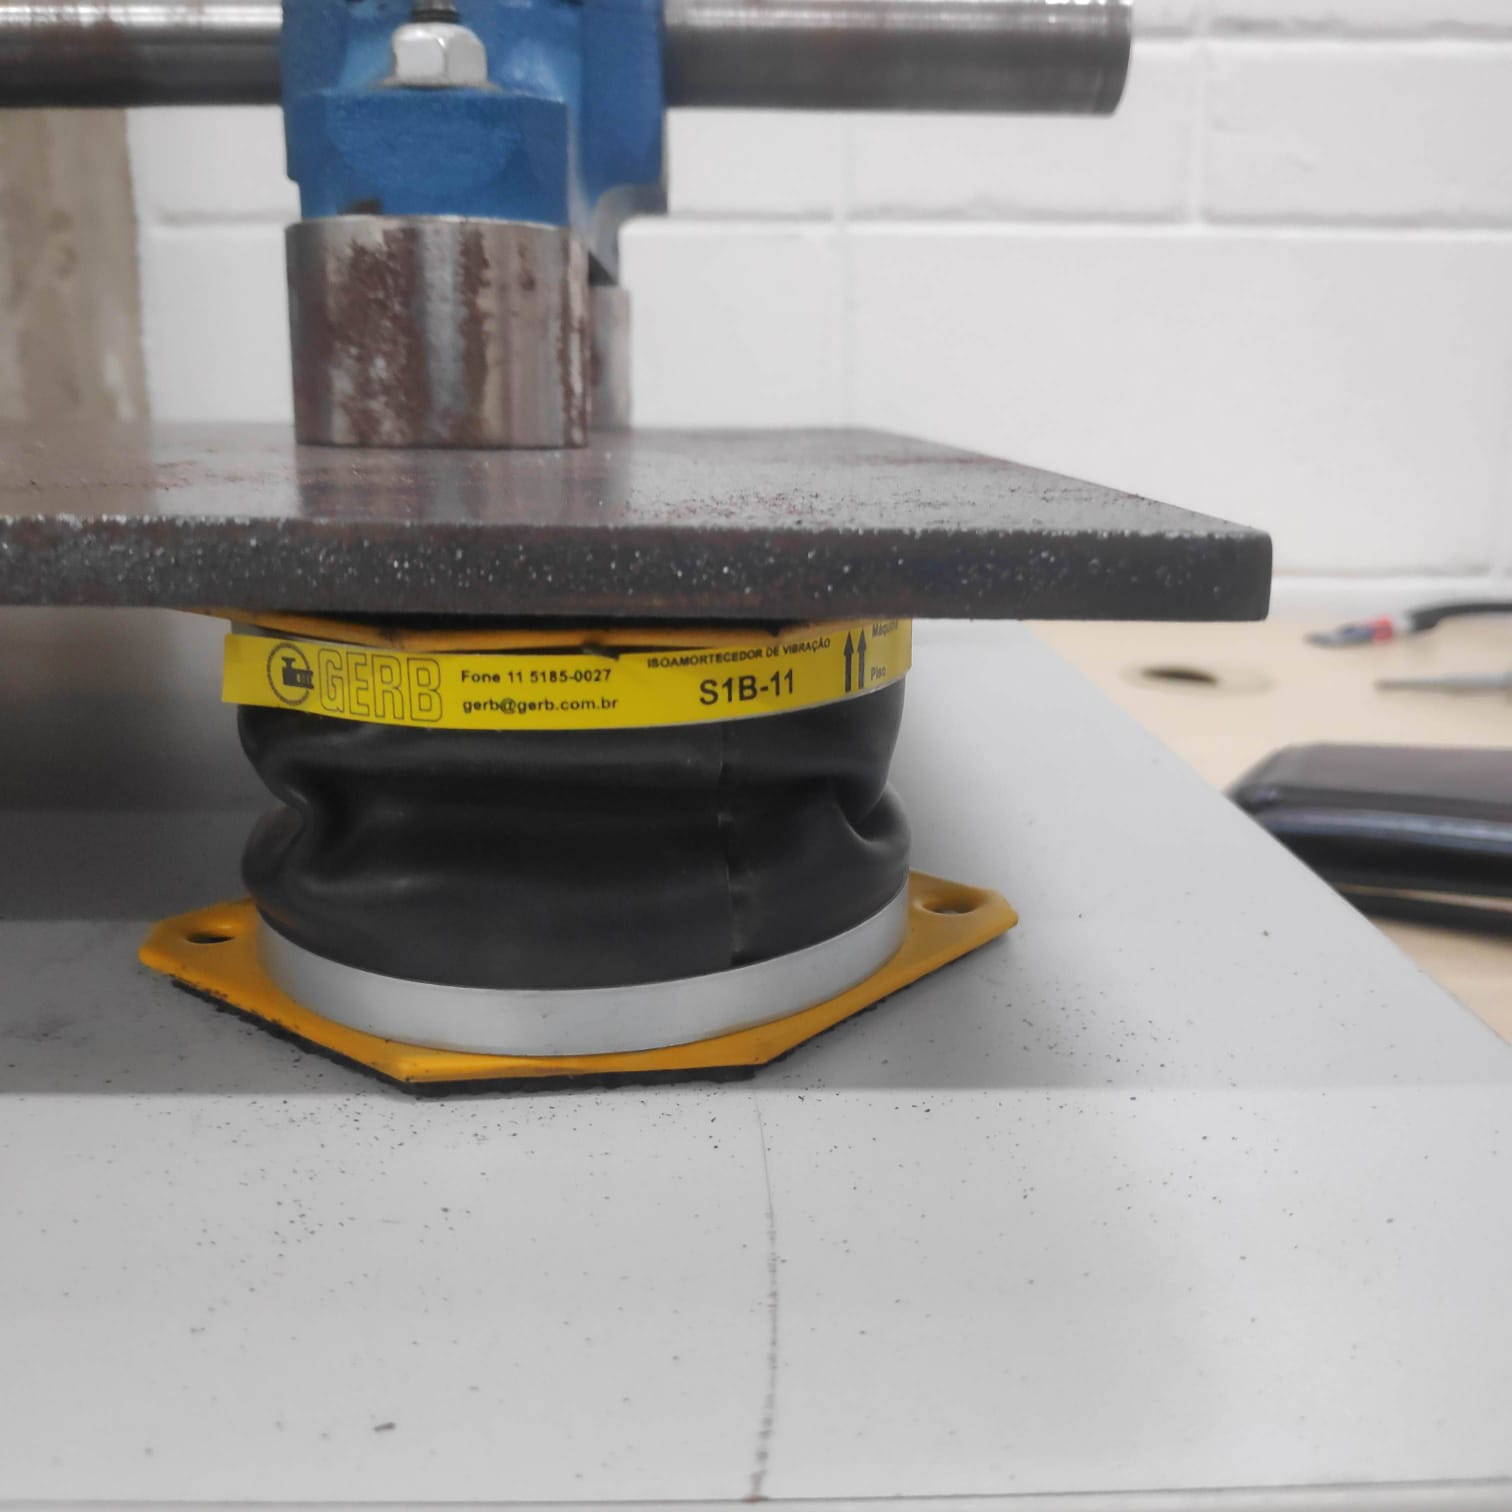
\includegraphics[width=\textwidth,height=70mm,keepaspectratio]{isoamortecedor_bancada}
\label{isoamortecedor_bancada}
\end{figure}


O motor utilizado na bancada de testes possui como características um torque de \SI{400}{\newton\metre}, velocidade de 1750 RPM com taxa de redução de 48,90 vezes, resultante em velocidade de saída para o eixo de 35,8 RPM. A medição com Tacômetro em partida direta mostrou uma taxa de rotação do eixo de 37 RPM. 

\begin{figure}[H]
\centering
\caption {Medição de rotação com partida direta. Elaborado pelo autor.}
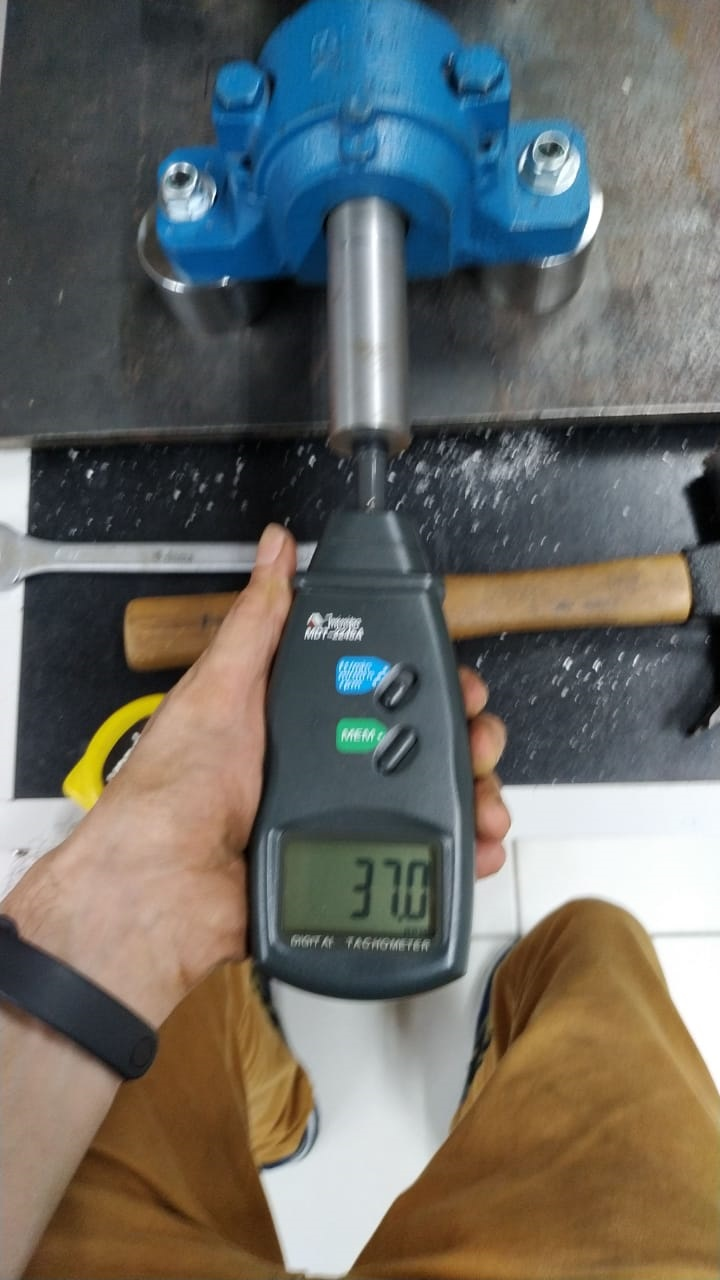
\includegraphics[width=\textwidth,height=100mm,keepaspectratio]{tacometro_lucas}
\label{tacometro_lucas}
\end{figure}
 
Também foi adicionado, para controle da bancada, um painel conforme mostrado na Figura~\ref{painel_bancada}. 

\begin{figure}[H]
\centering
\caption {Painel de controle da bancada experimental. Elaborado pelo autor.}
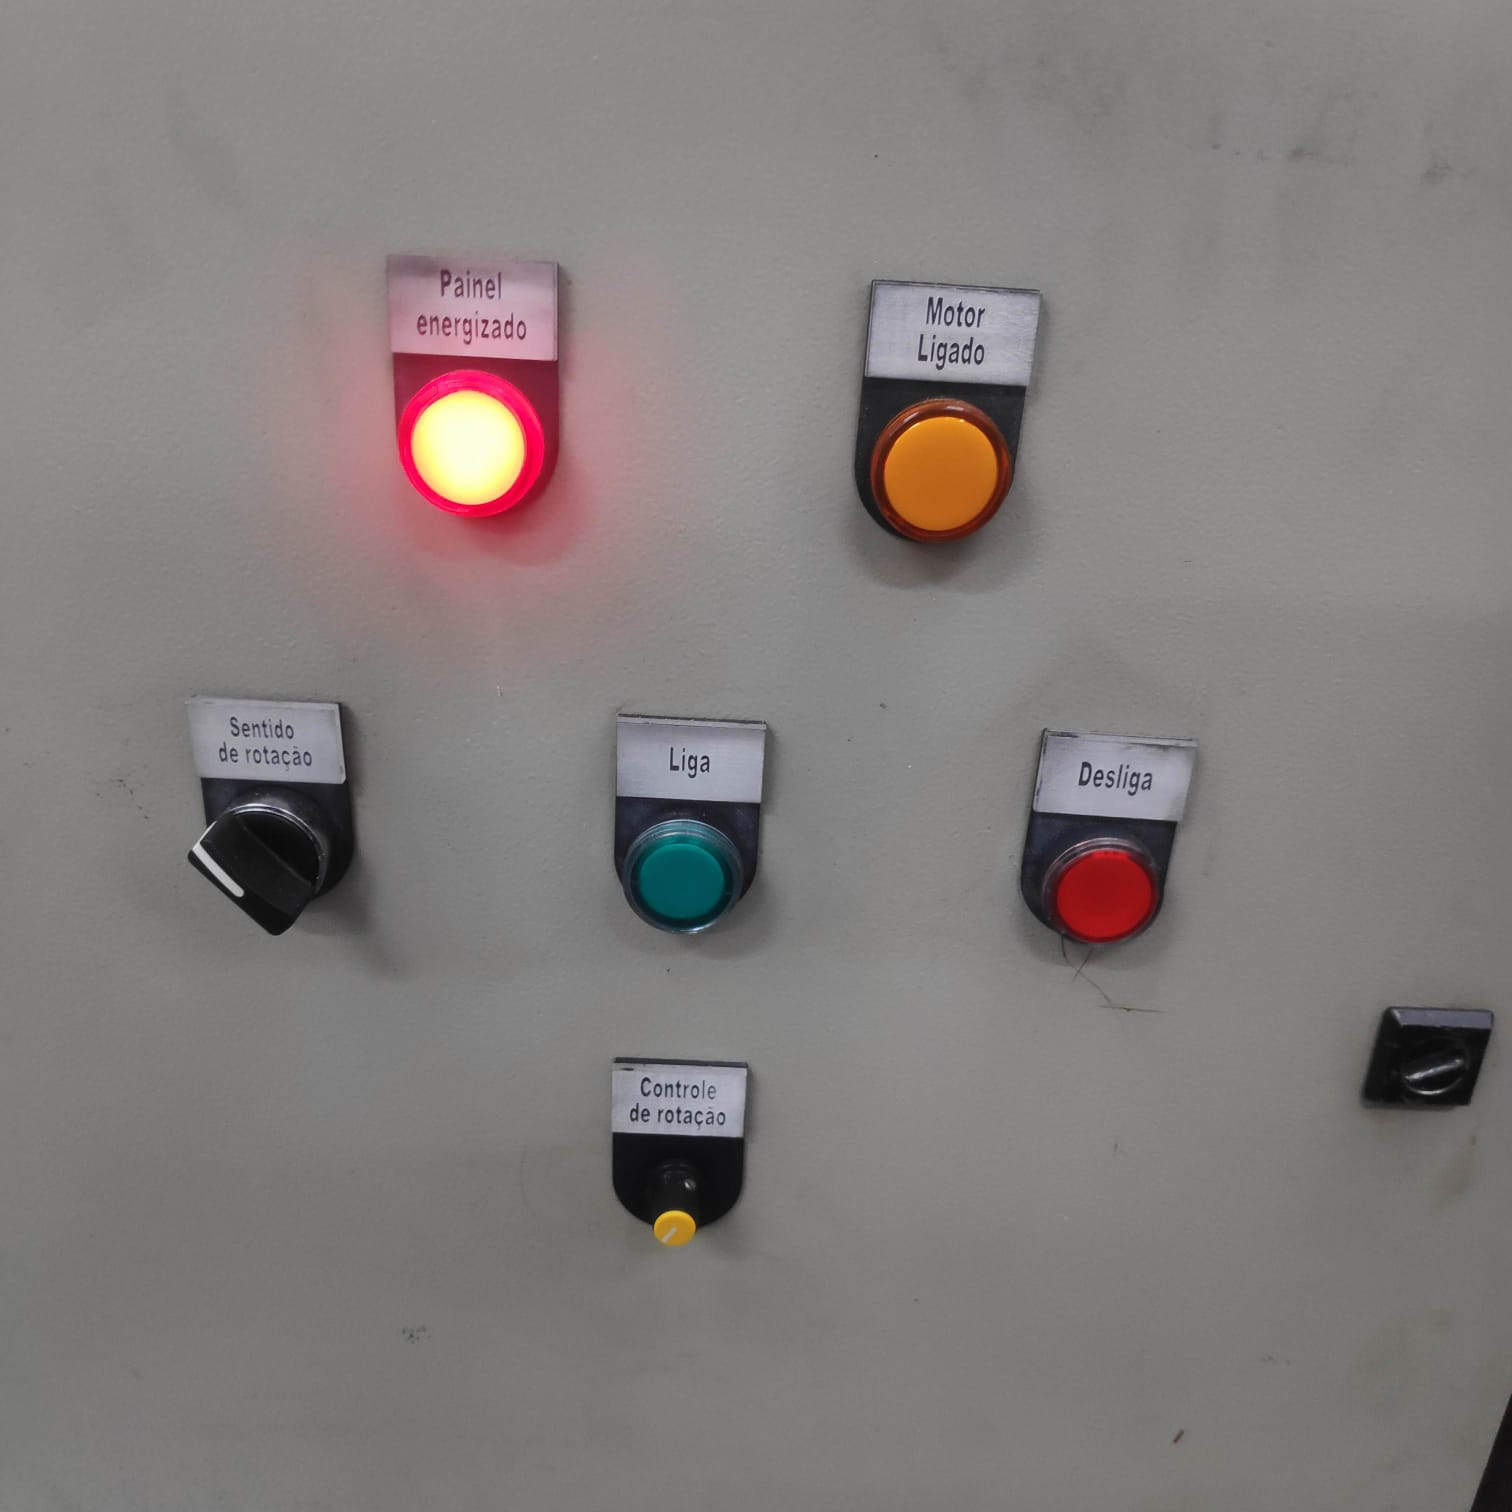
\includegraphics[width=\textwidth,height=90mm,keepaspectratio]{painel_bancada}
\label{painel_bancada}
\end{figure}
 
O painel é composto por botões indicadores iluminados por led indicando o estado da máquina: energizada ou não-energizada, com motor ligado ou desligado. Além disso há botões de controle para ligar e desligar a máquina, bem como ma chave seletora da direção de rotação e um potênciometro para controle da velocidade da rotação do eixo através de um dispositivo inversor de frequências. A Figura~\ref{painel_por_dentro} mostra a parte interna do painel.
 
\begin{figure}[H]
\centering
\caption {Inversor de frequências e instalação elétrica do painel da bancada experimental. Elaborado pelo autor.}
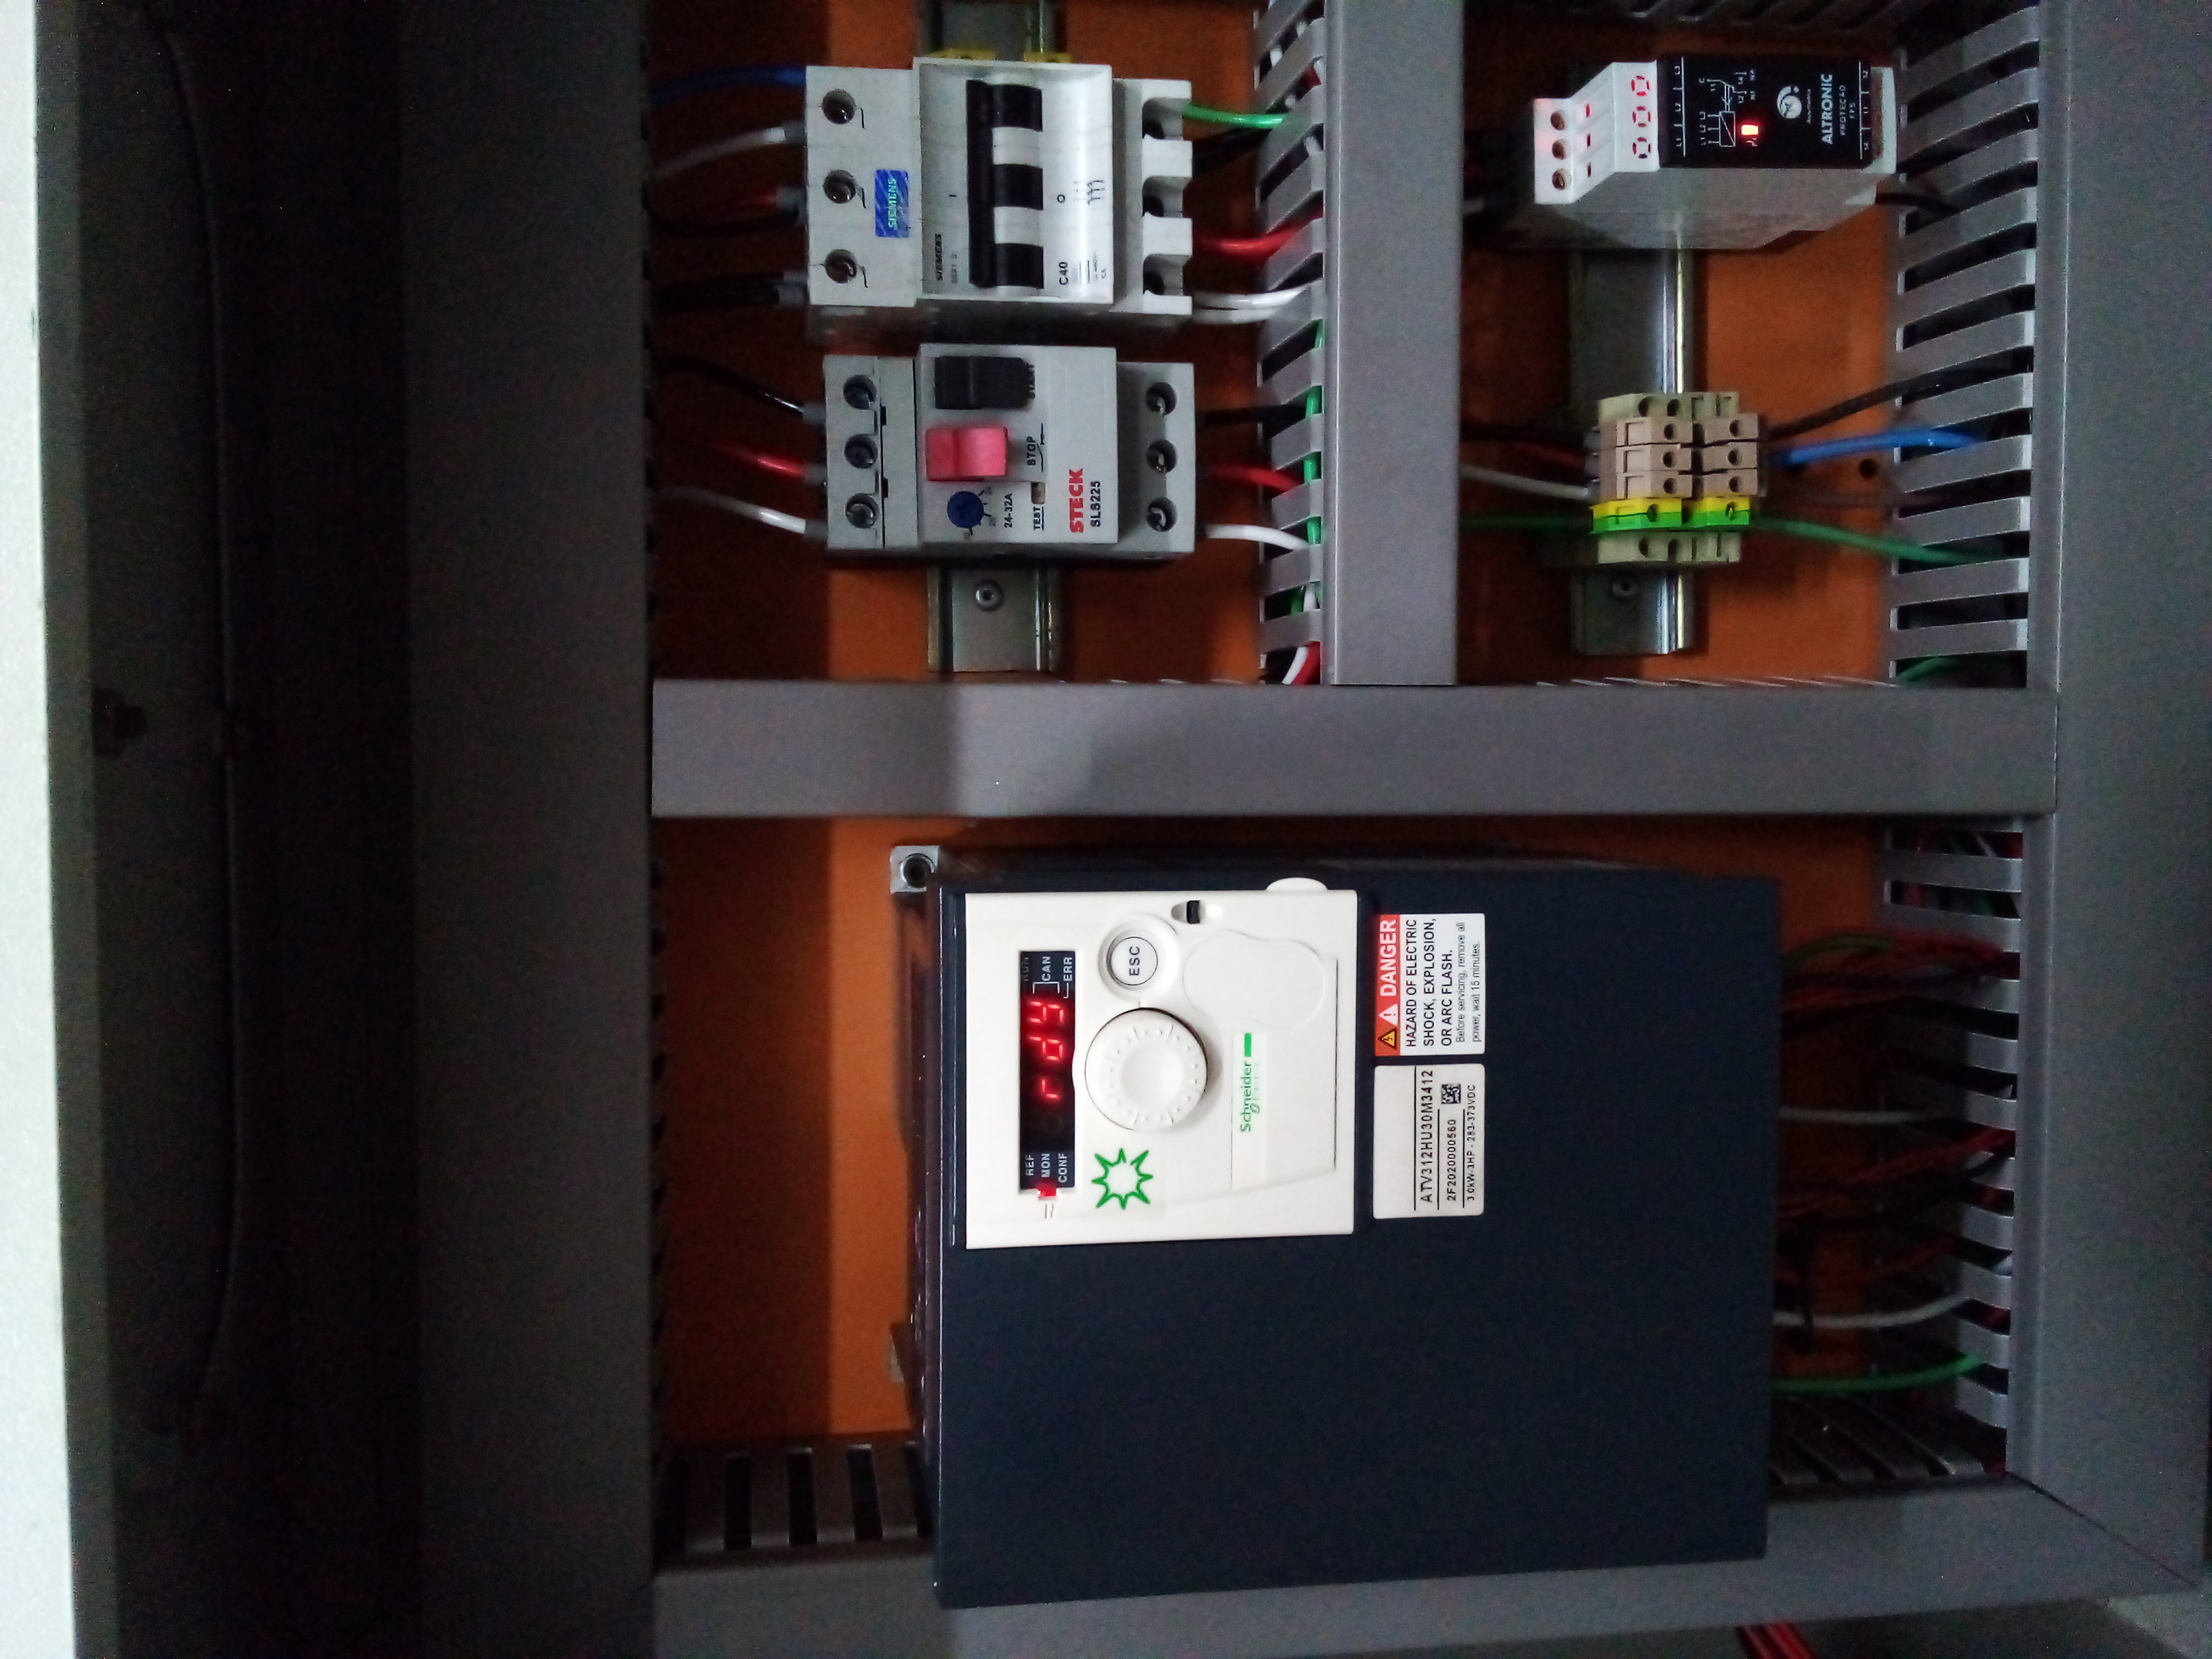
\includegraphics[width=\textwidth,height=100mm,keepaspectratio]{painel_por_dentro}
\label{painel_por_dentro}
\end{figure}

Além disso, também foi adicionado um acoplamento ao eixo, a fim de se diminuir interferências da vibração do dispositivo motorreduutor nos rolamentos. A Figura~\ref{acoplamento_eixo} mostra o acoplamento colocado no eixo. 

\begin{figure}[H]
\centering
\caption {Inversor de frequências e instalação elétrica do painel da bancada experimental. Elaborado pelo autor.}
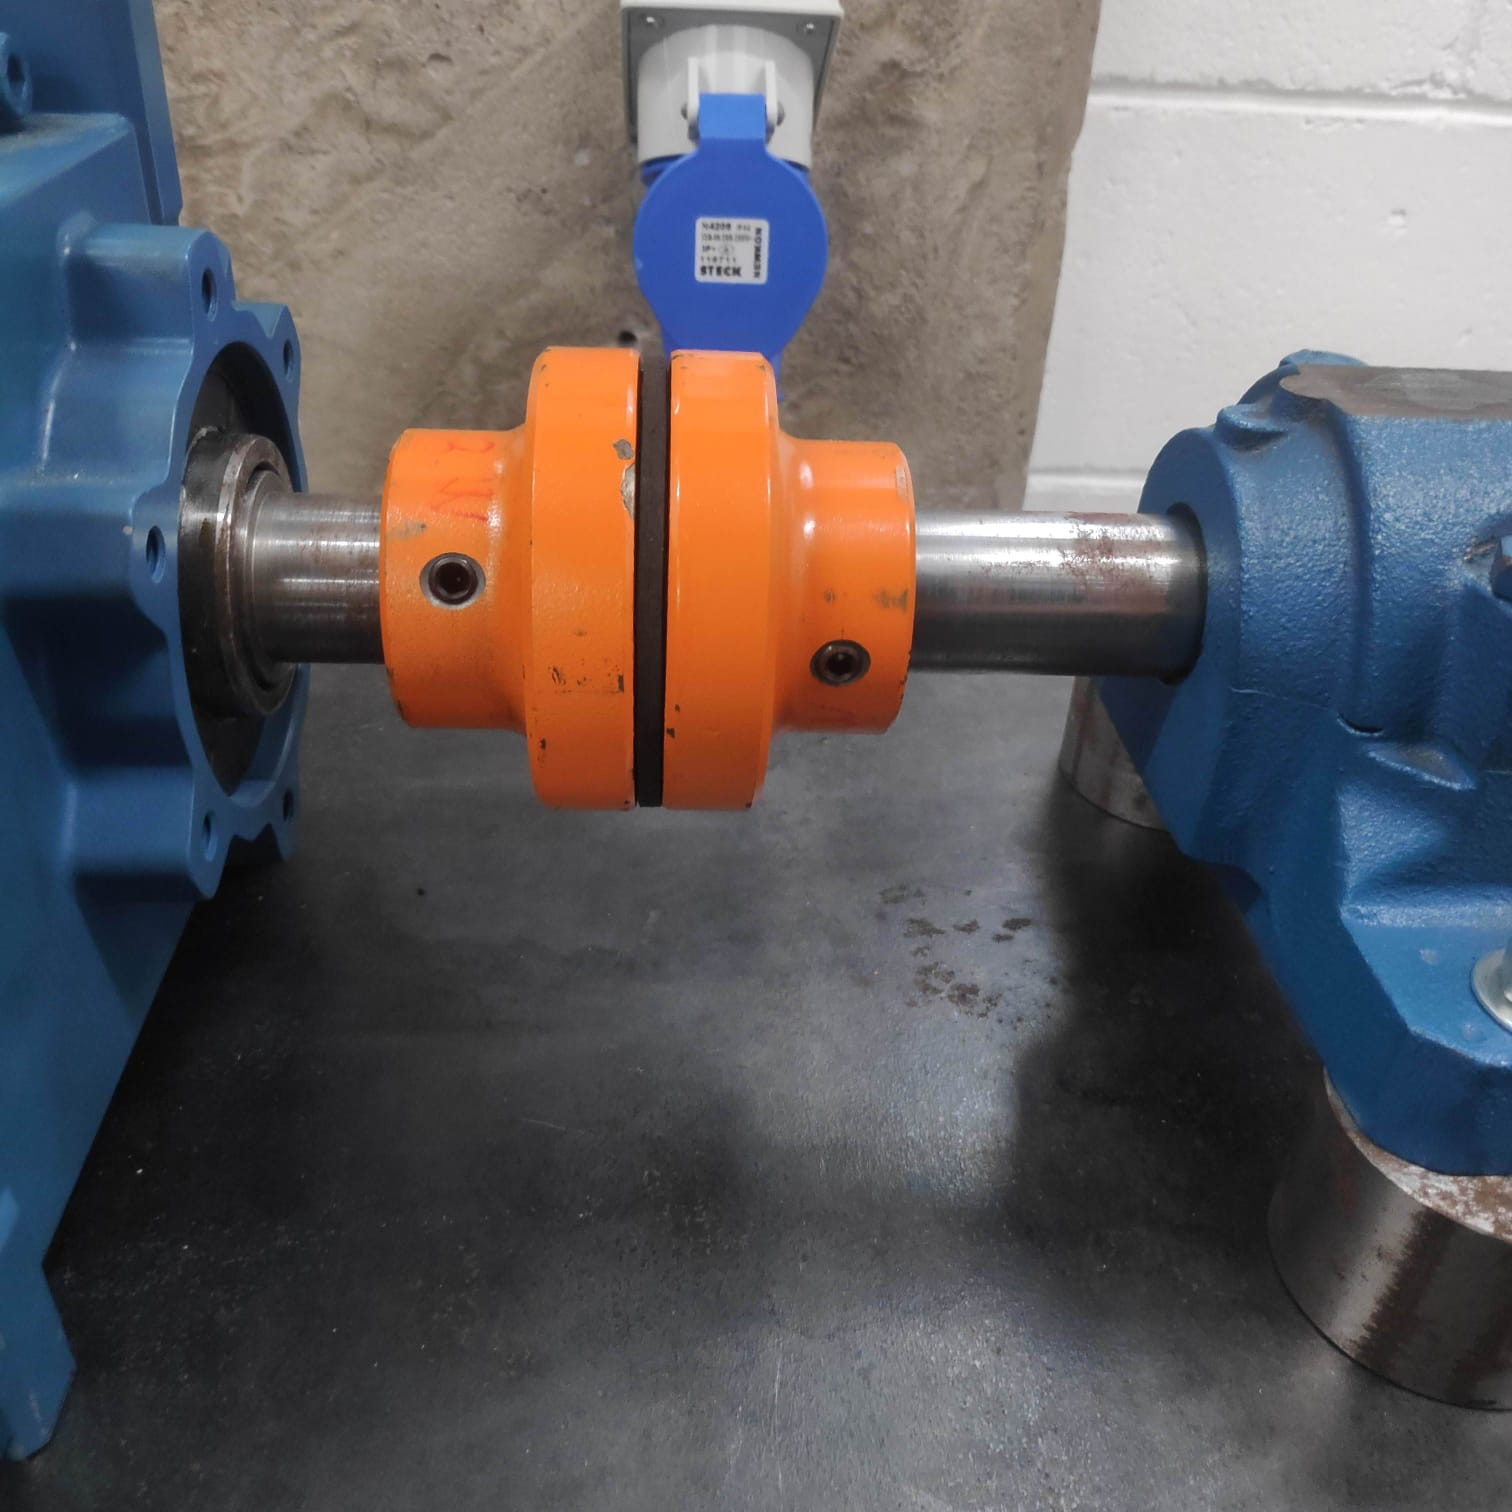
\includegraphics[width=\textwidth,height=90mm,keepaspectratio]{acoplamento_eixo}
\label{acoplamento_eixo}
\end{figure}
 
A Figura~\ref{bancada_aberta} mostra a bancada experimental visualizada com a porta do painel aberta e o inversor de frequências à mostra.
 
\begin{figure}[H]
\centering
\caption {Inversor de frequências e instalação elétrica do painel da bancada experimental. Elaborado pelo autor.}
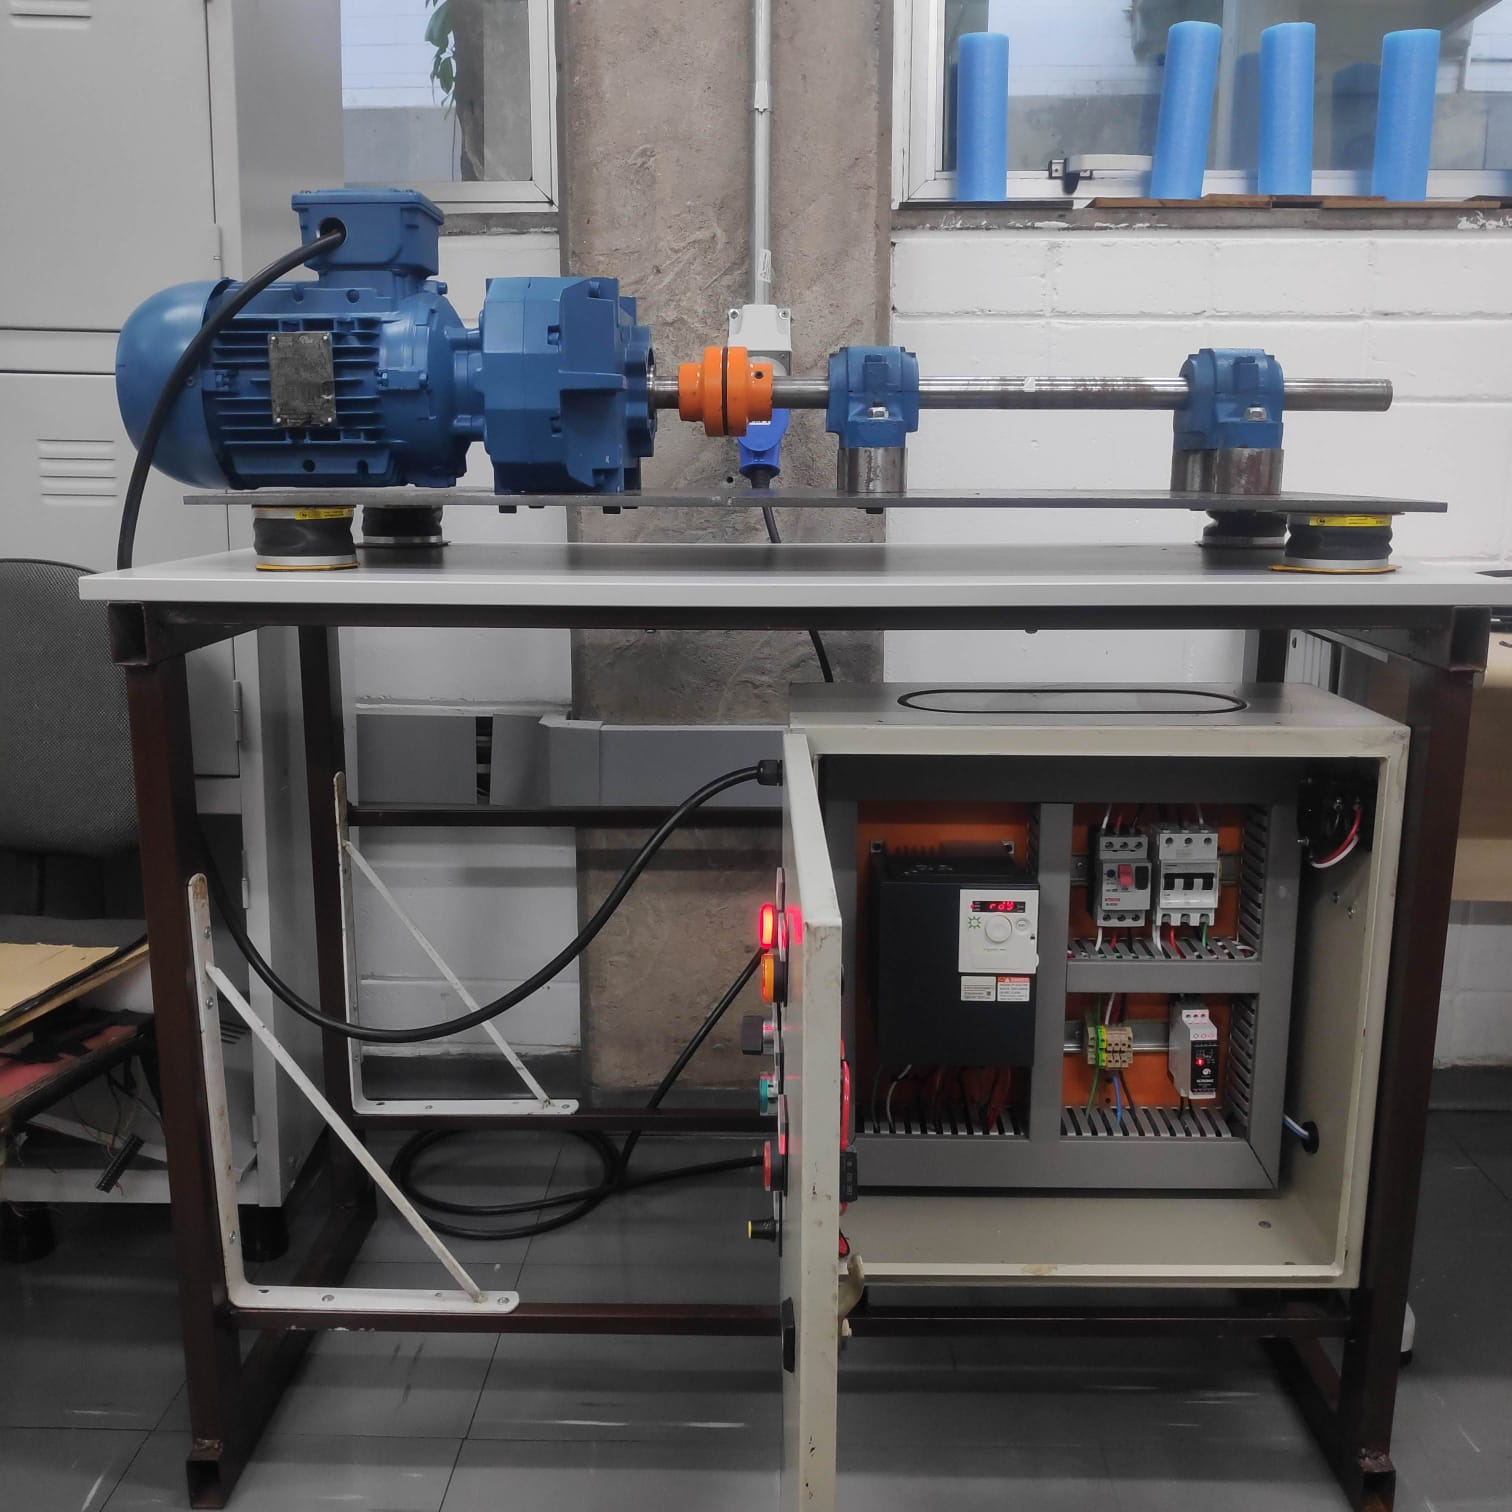
\includegraphics[width=\textwidth,height=100mm,keepaspectratio]{bancada_aberta}
\label{bancada_aberta}
\end{figure}
  

 
\section{\normalfont{\textbf{Cálculo das frequências esperadas}}}

A partir destes dados, pode-se calcular com base nas frequências características de defeitos as frequências esperadas de defeito para o rolamento adotado no estudo. O diâmetro primitivo $D$ se dá por: 

\begin{equation}
	D = \frac{\SI{72}{\mm} \ + \SI{30}{\mm}}{2} = \SI{51}{\mm}
	\label{eq: Diametro Primitivo no Rolamento}
\end{equation}


%\[D = \frac{\SI{72}{\mm} \ + \SI{30}{\mm}}{2} = \SI{51}{\mm} \]  

Logo, para a \textit{Fundamental Train Frequency} temos, aproximadamente:

\begin{equation}
	FTF = \frac{35}{2} \left ( 1 - \frac{10.1}{51} \,cos \, \ang{14} \right )  \ = \SI{~14}{{\hertz}}
	\label{eq: FTF no  Rolamento}
\end{equation}

%\[FTF = \frac{35}{2} \left ( 1 - \frac{10.1}{51} \,cos \, \ang{14} \right )  \ = \SI{~14}{{\hertz}} \]  

Para a \textit{Ball Pass Frequency of The Inner Race} temos, aproximadamente:

\begin{equation}
	BPFI = \frac{10}{2}35 \left ( 1 + \frac{10.1}{51} \,cos \, \ang{14} \right )  \ = \SI{~208}{{\hertz}}
	\label{eq: BPFI no rolamento}
\end{equation}

%\[BPFI = \frac{10}{2}35 \left ( 1 + \frac{10.1}{51} \,cos \, \ang{14} \right )  \ = \SI{~208}{{\hertz}} \]

Para a \textit{Ball Pass Frequency of The Outer Race} temos, aproximadamente:

\begin{equation}
	BPFO = \frac{10}{2}35 \left ( 1 - \frac{10.1}{51} \,cos \, \ang{14} \right )  \ = \SI{~141}{{\hertz}}
	\label{eq: BPFO no Rolamento}
\end{equation}

%\[BPFO = \frac{10}{2}35 \left ( 1 - \frac{10.1}{51} \,cos \, \ang{14} \right )  \ = \SI{~141}{{\hertz}} \]

Por fim, para a \textit{Ball Spin Frequency} temos, aproximadamente:

\begin{equation}
	BSF = \frac{51}{2*10.1}35 \Bigg[  1 - \left ( \frac{10.1}{51} \,cos \, \ang{14} \right ) ^{2}  \Bigg] \ = \SI{~85}{{\hertz}} \
	\label{eq: BSF no rolamento}
\end{equation}

%\[BSF = \frac{51}{2*10.1}35 \Bigg[  1 - \left ( \frac{10.1}{51} \,cos \, \ang{14} \right ) ^{2}  \Bigg] \ = \SI{~85}{{\hertz}} \]

\section{\normalfont{\textbf{Aquisição e análise do sinal do filme PVDF}}}

A partir destas frequências pode-se estimar as áreas para análise do sinal aquisitado, bem como realizar o tratamento e filtragem do sinal resultante do sensor a fim de eliminação de interferências eletromagnéticas. 

Serão aquisitados sinais de todas as amostras com defeitos, com a utilização de sensores fabricados com o polímero PVDF, com terminais que permitem a medição da sua diferença de potencial, quando estes estiverem sujeitos a um esforço mecânico. 

Tendo em vista se tratarem de sensores de alta impedância, se faz necessário isolamento elétrico, a fim de mitigar as interferências da fase da rede elétrica e de sinais de rádio incidentes sobre o local de testes, bem como tratamento da tensão resultante de esforço mecânico através de amplificação do sinal. 

Para tanto, utiliza-se um encapsulamento construído em alumínio, onde se acomoda o filme PVDF, além de amplificador operacional Texas Instruments LM2904, filtro passa alta e filtro passa baixa com regulagem de frequências variáveis. A Figura~\ref{Figura21} mostra o sensor de vibração. 

\begin{figure}[H]
\centering
\caption {Sensor de vibração piezoelétrico. Retirado de Measurement Specialties, 2021.}
\includegraphics[width=\textwidth,height=70mm,keepaspectratio]{Figura21}
\label{Figura21}
\end{figure} 

A montagem dos sensores se deu em um encapsulamento de alumínio. Estes são acoplados com cola acrílica, a fim de que não ocorra amortecimento da vibração devido ao elemento colante. Uma vez montado o aparato, os sinais decorrentes da vibração são aquisitados para posterior comparação com os sinais característicos dos rolamentos sem defeitos a fim de que se determine a severidade da falha. A Figura~\ref{encapsulamento_sensor} mostra uma montagem do sensor em seu encapsulamento.

\begin{figure}[H]
\centering
\caption {Sensor de vibração piezoelétrico no encapsulamento de alumínio. Elaborado pelo autor.}
\includegraphics[width=\textwidth,height=75mm,keepaspectratio]{encapsulamento_sensor}
\label{encapsulamento_sensor}
\end{figure} 

A Figura~\ref{circuito_sensor} mostra o circuito preliminar de condicionamento do sensor piezoelétrico, elaborado no \textit{software} Proteus. Neste buscou-se a amplificação do sinal, tendo se optado pelo amplificador operacional de propósito geral Texas Instruments LM2904, uma vez que este possui dois canais e larga banda de \SI{1}{\mega\hertz} (Texas Instruments, 2021). Os valores dos componentes deste circuito serão alterados a partir das informações obtidas nos testes.

\begin{figure}[H]
\centering
\caption {Circuito preliminar de condicionamento do sensor piezoelétrico. Elaborado pelo autor.}
\includegraphics[width=\textwidth,height=\textheight,keepaspectratio]{circuito_sensor}
\label{circuito_sensor}
\end{figure} 

Para a aquisição de dados, foi construído software de aquisição baseado no microcontrolador STM32, modelo stm32f103, também conhecido como \textit{bluepill}. Este foi utilizado por se tratar de um microcontrolador largamente disponível no mercado, de baixo custo, com \SI{72}{\mega\hertz} de velocidade de CPU e 20KB de memória RAM, também possuindo conversor analógico digital com resolução de 12 bits. 

\begin{figure}[H]
\centering
\caption {Microcontrolador STM32F103. Retirado de ST, 2021.}
\includegraphics[width=\textwidth,height=50mm,keepaspectratio]{stm32}
\label{stm32}
\end{figure}

O software foi desenvolvido em linguagem C, com utilização dos registradores do microcontrolador e testado com dispositivo gerador de função. A Figura~\ref{medidas_sistema_aquisicao_stm32} mostra a aquisição de um sinal de \SI{5}{\kilo\hertz}, representado através de forma de onda. Para a aquisição do sinal dos rolamentos optou-se por uma taxa de \SI{51,6}{\kilo\hertz}, ou seja, 2,56 vezes a frequência limite de interesse de \SI{20}{\kilo\hertz} inicialmente adotada. 

\begin{figure}[H]
\centering
\caption {Sinal de \SI{5}{\kilo\hertz} capturado pelo sistema construído com o microcontrolador STM32. Elaborado pelo autor.}
\includegraphics[width=\textwidth,height=\textheight,keepaspectratio]{medidas_sistema_aquisicao_stm32}
\label{medidas_sistema_aquisicao_stm32}
\end{figure} 

Os modelos matemáticos de identificação de frequências características de defeitos serão utilizados para a análise dos sinais no domínio do tempo e da frequência, que terão a finalidade de calibragem dos níveis de alarme. Para fins de validação dos dados obtidos através do sistema de aquisição desenvolvido com a plataforma STM32, será utilizado a DAQ da National Instruments modelo USB-6212. Esta conta com integração total ao sistema LabView, largamente utilizado na indústria e que será, aqui, utilizado para construção de um sistema com finalidade comparativa. A Figura~\ref{sistema_labview} apresenta o sistema desenvolvido para tanto, na versão livre para uso acadêmico do LabView 2020.

\begin{figure}[H]
\centering
\caption {Sistema de aquisição desenvolvido com LabView. Elaborado pelo autor.}
\includegraphics[width=\textwidth,height=\textheight,keepaspectratio]{sistema_labview}
\label{sistema_labview}
\end{figure} 

Após a captura dos dados, a análise se dará através de nível RMS e Transformada rápida de Fourier. Para a análise dos dados aquisitados através do sistema desenvolvido com o STM32 será utilizada a plataforma Pandas, construída na linguagem de programação python, bem como também mantém-se aberta a possibilidade de utilização da plataforma Octave, alternative livre ao sistema Matlab. Estas são ferramentas de software livre, com licenças do tipo BSD. 

A Figura~\ref{fluxograma_aquisicao} apresenta o fluxo de como se dará o processo.

\begin{figure}[H]
\centering
\caption {Fluxo de aquisição e processamento. Elaborado pelo autor.}
\includegraphics[width=\textwidth,height=60mm,keepaspectratio]{fluxograma_funcionamento_sistema}
\label{fluxograma_aquisicao}
\end{figure} 

%A depender da qualidade dos resultados preliminares, em particular os níveis de sinal obtidos e quantidade de ruído capturada, admite-se a possibilidade de se fazer necessário empregar os níveis de Curtose e Densidade espectral de potência.  

%Por fim, os custos dos sensores fabricados em PVDF serão calculados e comparados com os equipamentos atualmente disponíveis para aferição do custo vs benefício, visando com esta ação reduzir a ocorrência de falhas catastróficas, que são um grande risco tanto para a segurança dos operadores de máquinas quanto para a saúde financeira das empresas pela parada não programada da produção.

A análise dos resultados obtidos se dará à luz da revisão bibliográfica e comparativamente com os resultados encontrados em outros artigos. 

\section{\normalfont{\textbf{Circuitos condicionadores do sinal}}}
\label{secao:CircuitosCondicionadores}

A partir de testes iniciais verificou-se que o sensor, por ser de alta impedância, apresentava altos níveis de ruído. Assim, foram projetados e construídos circuitos condicionadores de sinal para o trabalho com o sensor PVDF.  

A Figura~\ref{sinal_filtrado_maquina_desligada} compara os sinais pré-filtragem e pós-filtragem do sensor: em vermelho, o sinal saído diretamente do amplificador operacional sem filtragem; em branco, o sinal filtrado pelo filtro notch rejeita-faixa. 

\begin{figure}[H]
\centering
\caption {Elaborado pelo autor.}
\includegraphics[width=\textwidth,height=90mm,keepaspectratio]{GraficosAnalise/sinal_filtrado_maquina_desligada}
\label{sinal_filtrado_maquina_desligada}
\end{figure} 



\section{\normalfont{\textbf{Definição dos experimentos}}}

A definição dos experimentos se deu por diferentes cenários: 1) cenário de aquisições sem qualquer tipo de filtro, apenas com amplificação por meio de amplificador operacional; 2) cenário de aquisições com filtragem analógica utilizando-se do circuito construído e descrito na seção X – Materiais e Métodos; 3) cenário baseado em filtragem analógica seguido de filtragem digital implementada através da plataforma LabVIEW.

A definição destes cenários distintos se deu a partir da necessidade de se avaliar o sinal gerado pelo sensor, acoplado à caixa de rolamento, enquanto sujeito níveis de interferências eletromagnéticas com e sem filtragem. Tal definição se deu pois verificou-se, inicialmente, uma quantidade perceptível de interferências eletromagnéticas no sensor, conforme descrito na seção~\ref{secao:CircuitosCondicionadores}

Durante a fase de aquisição dos dados, também foi realizado um conjunto de aquisições com utilização de um filtro digital rejeita-faixa do tipo Butterworth de 4ª ordem, implementado através da plataforma LabVIEW, bem como um filtro passa-baixa também do tipo Butterworth de 4ª ordem. Tal implementação se deu com o objetivo de mitigar interferências verificadas acima dos 2500Hz e, também, interferências ainda presentes por volta dos 60Hz – frequência das oscilações da corrente alternada. 

Além destas interferências outras foram verificadas, através da análise espectral por meio de FFT, na própria placa de aquisição USB-6212, conforme visto na Figura 1.

Dentre os possíveis motivos para tal interferência, estima-se que estes sejam decorrentes de ruídos provenientes da própria fonte do computador utilizado para aquisição dos dados, a qual pode interferir na porta USB utilizada para conexão do dispositivo de aquisição. Entretanto verificou-se, após a inclusão do filtro digital, que o mesmo atenuou demasiadamente o sinal, tendo funcionado como um passa-baixa ao invés de um passa-faixa. 

Inicialmente as análises foram feitas com os sinais obtidos com utilização do filtro analógico e sem qualquer filtragem, apenas com amplificação proveniente do amplificador operacional. Após isto, foram feitas análises com inclusão dos filtros digitais. 

Para condução da aquisição destes distintos cenários as taxas de aquisição foram baseadas nos modelos encontrados em outros artigos, tais como FULANO et al, XXXX. Tais taxas respeitam o critério de Nyquist para representação do espectro de frequências de interesse. Optou-se pela captura, nas taxas de aquisição descritas na Tabela , por dois minutos ininterruptos em cada caso – tempo suficiente para captura de um conjunto de rotações do eixo e, portanto, da assinatura dos danos nos rolamentos. 

Desta forma, os parâmetros de aquisição dos dados analisados até o momento foram definidos e encontram-se na Tabela 1

\chapter{Resultados}

Nesta seção são apresentados os resultados dos experimentos realizados com o sensor filme PVDF.

\section{\normalfont{\textbf {Caso 1 - caracterização do sinal do sensor}}}

Para caracterização do sinal inerente ao sensor, submetido ao circuito de condicionamento e filtragem do sinal, foram feitos os seguintes experimentos: 1) aquisição do sinal do sensor com o maquinário desligado e desconectado da energia elétrica; 2) aquisição com o maquinário desligado, mas conectado à tomada; 3) maquinário energizado, mas com motor parado. A finalidade destes experimentos foi de, inicialmente, verificar o nível de ruído do sinal em termos de interferências eletromagnéticas no ambiente.

Para que se conduzissem os experimentos deste cenário o sensor foi posicionado no rolamento e seu sinal aquisitado a uma taxa igual a taxa de aquisição dos ensaios. A tabela 

Estes três cenários distintos propostos visaram a verificação da amplitude de ruídos elétricos que ainda fossem capaz de interferências no sinal. 

A Figura~\ref{maquina_desligada_da_tomada} mostra o sinal temporal da bancada de ensaios desconectado da energia elétrica. 

\begin{figure}[H]
\centering
\caption {Sinal temporal da bancada desconectada da energia elétrica. Elaborado pelo autor.}
\includegraphics[width=\textwidth,height=90mm,keepaspectratio]{Caso0/maquina_desligada_da_tomada}
\label{maquina_desligada_da_tomada}
\end{figure} 

O sinal temporal aponta a presença de um ruído, com amplitude pico a pico de aproximadamente {\SI{8}{\milli\volt}}. Calculando-se o FFT e o PSD do sinal, foi obtido o resultado mostrado na Figura~\ref{PSD_SENSOR_MAQUINA_DESLIGADA}. 

\begin{figure}[H]
\caption {Espectro do sinal da bancada desconectada da energia elétrica. Elaborado pelo autor.}
\includegraphics[height=95mm,keepaspectratio]{Caso0/PSD_SENSOR_MAQUINA_DESLIGADA}
\label{PSD_SENSOR_MAQUINA_DESLIGADA}
\end{figure} 

Através da remoção do componente de corrente contínua do sinal, foi possível verificar quais frequências o compõe. Foi possível verificar que o espectro possui um elevado pico na região dos {\SI{60}{\hertz}, sem alterações nas demais faixas de frequência. Considerando-se que apenas o filtro rejeita-faixa estava ligado à energia neste momento, conclui-se que o referido ruído foi induzido pela própria fonte de alimentação do mesmo. Ou seja, ainda que o circuito condicionador, em conjunto com o filtro, tenha sido capaz de atenuar as componentes de interferência elétrica, componentes de ruído elétrico ainda se mostraram presentes. 

A partir deste cenário, para que se verificasse o quanto estes sinais seriam presentes nas componentes de frequência durante o processo de aquisição dos dados, foi proposto o experimento de aquisição dos dados com a bancada ligada a tomada, mas não energizada. A Figura~\ref{maquina_ligada_na_tomada} mostra o sinal temporal da bancada quando conectada à energia elétrica.

\begin{figure}[H]
\centering
\caption {Sinal temporal da bancada conectada à energia elétrica. Elaborado pelo autor.}
\includegraphics[width=\textwidth,height=90mm,keepaspectratio]{Caso0/maquina_ligada_na_tomada}
\label{maquina_ligada_na_tomada}
\end{figure} 

A partir do sinal temporal deste experimento foi possível verificar o incremento na amplitude do sinal, bem como novos componentes de frequência induzidos. A amplitude de tensão pico a pico cresceu para aproximadamente {\SI{20}{\milli\volt}}, mais que dobrando em relação ao experimento anterior. A Figura~\ref{PSD_SENSOR_MAQUINA_LIGADA} mostra as componentes deste sinal, composto tanto pelos {\SI{60}{\hertz} anteriormente identificados quanto por uma nova componente de alta frequência, centrada na faixa dos {\SI{9500}{\hertz}. A origem desta nova componente de alta frequência não pôde ser identificada. 

\begin{figure}[!htb]
\centering
\caption {Elaborado pelo autor.}
\includegraphics[width=170mm,keepaspectratio]{Caso0/PSD_SENSOR_MAQUINA_LIGADA}
\label{PSD_SENSOR_MAQUINA_LIGADA}
\end{figure} 

Estas interferências, conclui-se, se devem à natureza de alta impedância do sensor PVDF.  

Assim, verificando-se o aumento dos sinais de interferência elétrica ao ligar a bancada na energia elétrica, foi proposto o experimento de aquisição dos dados com a bancada energizada, mas não em funcionamento. A Figura~\ref{maquina_ligada_na_tomada_e_energizada} mostra o sinal temporal deste caso.

\begin{figure}[H]
\centering
\caption {Elaborado pelo autor.}
\includegraphics[width=\textwidth,height=90mm,keepaspectratio]{Caso0/maquina_ligada_na_tomada_e_energizada}
\label{maquina_ligada_na_tomada_e_energizada}
\end{figure} 

É possível verificar, neste caso, o aumento da amplitude pico a pico dos sinais, superior a {\SI{25}{\milli\volt}}. Já em relação ao sinal espectral deste caso, como é possível visualizar na Figura~\ref{PSD_SENSOR_MAQUINA_LIGADA_E_ENERGIZADA}, o mesmo aponta picos na região dos {\SI{60}{\hertz} e dos {\SI{9500}{\hertz}. Nota-se, entretanto, que ao contrário do experimento anterior, onde as interferências de alta frequência dominavam o espectro em termos de amplitude, neste experimento a frequência da corrente alternada volta a ser dominante. Isto ocorre pela indução causada pelos demais elementos da bancada de testes, agora energizados, tal como o inversor de frequências.   

\begin{figure}[H]
\centering
\caption {Elaborado pelo autor.}
\includegraphics[width=170mm,keepaspectratio]{Caso0/PSD_SENSOR_MAQUINA_LIGADA_E_ENERGIZADA}
\label{PSD_SENSOR_MAQUINA_LIGADA_E_ENERGIZADA}
\end{figure} 

Os resultados desta caracterização de ruídos encontram-se sumarizados na Tabela~\ref{tab:caraterizaçãoSinal}

\begin{table}[h]
\caption{Caracterização do ruído elétrico capturado pelo sistema}
\begin{tabularx}{\textwidth}{|X|X|X|X|}
\hline
Caracterização do ruído do sensor               & Valor pico a pico    & Valor RMS & Frequências dominantes                                                               \\ \hline
Bancada desligada da energia elétrica           & Aproximadamente 8mv  &           & Espectro com pico nos 60Hz                                                           \\ \hline
Bancada ligada na energia elétrica              & Aproximadamente 20mv &           & Espectro demonstrando uma concentração de ruído nos 60Hz e pico por volta dos 9500Hz \\ \hline
Bancada ligada na energia elétrica e energizada & Aproxidamente 25mv   &           & Espectro demonstrando uma concentração de ruído nos 9500Hz e pico nos 60Hz           \\ \hline
\end{tabularx}
\label{tab:caraterizaçãoSinal}
\source{O autor (2022).}
\end{table}


\section{\normalfont{\textbf {Caso  2 - caracterização do sinal do motorredutor}}}

Após a caraterização das interferências elétricas que seriam inerentes ao sensor, o padrão de vibrações do motorredutor foi caracterizado, a fim de que fossem verificadas suas frequências. Isto foi necessário pois as frequências geradas pelo conjunto motorredutor não eram, à priori, conhecidas. Assim, para que se evitasse possíveis confusões ao se caracterizar os sinais de rolamentos, caso, por coincidência, alguma das frequências de defeito esperadas fossem iguais às do motorredutor, tal caracterização foi proposta. 

Para tanto o sinal foi aquisitado durante dois minutos ininterruptos, tendo sido processados e aqui apresentados, para manutenção da consistência com os demais comparativos realizados, os primeiros seis segundos do sinal. A Figura~\ref{motorredutor} mostra o referido sinal no domínio do tempo.

\begin{figure}[H]
\centering
\caption {Sinal temporal do motorredutor. Elaborado pelo autor.}
\includegraphics[width=\textwidth,height=100mm,keepaspectratio]{Caso0/motorredutor}
\label{motorredutor}
\end{figure} 

Percebe-se um incremento significativo nos valores de tensão pico a pico, quando comparado ao caso anterior com a bancada meramente energizada, atingindo por volta de {\SI{1}{\volt}}. Isto mostrou inicialmente uma evidência de que a relação sinal-ruído seria, portanto, positiva - ou seja, a tensão gerada pelo sinal mecânico seria superior à do ruído elétrico. 

Contudo, analisando-se o caso no domínio das frequências é possível notar, ao se analisar o PSD deste experimento, que as frequências dominantes ainda se mantém centradas nos ruídos anteriormente detectados. A Figura~\ref{PSD_MOTORREDUTOR} mostra os picos de energia contidos no sinal, destacados, ainda, nos {\SI{60}{\hertz} e também nos {\SI{9500}{\hertz}.

\begin{figure}[H]
\centering
\caption {Espectro de densidade de potência do motorredutor. Elaborado pelo autor.}
\includegraphics[width=\textwidth,height=100mm,keepaspectratio]{Caso0/PSD_MOTORREDUTOR}
\label{PSD_MOTORREDUTOR}
\end{figure}

Dado o ruído inerente ao sensor, adotou-se uma estratégia de filtragem manual através da análise da densidade espectral de potência, filtrando-se os ruídos com grande interferência no sinal.

Para que fosse possível visualizar onde as demais frequências estavam ocorrendo, foi realizado o processo de filtragem através do PSD. Foram excluídos, após inspeção visual, os picos acima de 0.2 W/Hz. Excluindo-se os picos significativos de ruídos, o resultado, então apresentou-se conforme visto na Figura~\ref{PSD_MOTORREDUTOR_FILTRADO}. 

\begin{figure}[H]
\centering
\caption {Espectro de densidade de potência do motorredutor com picos filtrados. Elaborado pelo autor.}
\includegraphics[width=\textwidth,height=100mm,keepaspectratio]{GraficosAnalise/PSD_MOTORREDUTOR_FILTRADO_ANOTADO}
\label{PSD_MOTORREDUTOR_FILTRADO_ANOTADO}
\end{figure}

A partir desta filtragem verifica-se uma predominância de frequências na região dos {\SI{3800}{\hertz} aos {\SI{4000}{\hertz}. 

Contudo, além deste também é possível verificar picos isolados por volta dos {\SI{128}{\hertz}, {\SI{360}{\hertz}, além de uma concentração de menor amplitude de frequências em {\SI{986}{\hertz} e outra, ainda menor, na região dos {\SI{1730}{\hertz}. 

As caracteristicas do sinal de vibração do motorredutor, portanto, são sumarizadas na tabela ... 

\section{\normalfont{\textbf {Caso 3 - caracterização do sinal do rolamento em bom estado}}}



O próximo experimento, após caracterização do sinal do motorredutor, foi a caracterização do sinal do rolamento autocompensador de rolos em bom estado, sem nenhum tipo de dano introduzido. 

A Figura~\ref{DOMINIO_TEMPO_ROLAMENTO_BOM} mostra o sinal temporal do rolamento em bom estado. 

\begin{figure}[H]
\centering
\caption {Sinal temporal do rolamento em bom estado. Elaborado pelo autor.}
\includegraphics[width=\textwidth,height=100mm,keepaspectratio]{Caso1/DOMINIO_TEMPO_ROLAMENTO_BOM}
\label{DOMINIO_TEMPO_ROLAMENTO_BOM}
\end{figure} 


A Figura~\ref{PSD_ROLAMENTO_BOM} apresenta o PSD do rolamento em bom estado.

\begin{figure}[H]
\centering
\caption {Espectro de densidade de potência do rolamento em bom estado. Elaborado pelo autor.}
\includegraphics[width=\textwidth,height=100mm,keepaspectratio]{GraficosAnalise/PSD_ROLAMENTO_BOM}
\label{PSD_ROLAMENTO_BOM}
\end{figure} 

Nele podemos verificar uma concentração de frequências por volta dos 

\newpage
\section{\normalfont{\textbf {Caso 4 - caracterização do sinal e identificação da frequência característica de defeitos no rolamento com dano no elemento rolante}}}

A partir destas caracterizações, é dado prosseguimento nos experimentos a fim de identificação de danos no rolamento. Neste experimento foi introduzido dano no elemento rolante, conforme 

A Figura ~\ref{DEFEITO_ELEMENTO_ROLANTE} mostra o sinal temporal do rolamento com dano no elemento rolante. 

\begin{figure}[H]
\centering
\caption {Sinal temporal do rolamento com dano no elemento rolante. Elaborado pelo autor.}
\includegraphics[width=\textwidth,height=100mm,keepaspectratio]{GraficosAnalise/DEFEITO_ELEMENTO_ROLANTE}
\label{DEFEITO_ELEMENTO_ROLANTE}
\end{figure} 

É possível verificar através do sinal temporal uma tensão pico a pico de aproximadamente {\SI{150}{\milli\volt}}. Observando-se a densidade espectral de potência, é possível verificar a existência de uma concentração iniciando-se nos {\SI{80}{\hertz} e indo até, aproximadamente, os {\SI{117}{\hertz}}, com pico nos {\SI{103}{\hertz}. Também há uma concentração, de menor amplitude, entre os {\SI{380}{\hertz} e os {\SI{408}{\hertz}, conforme mostra a Figura~\ref{PSD_DEFEITO_ELEMENTO_ROLANTE_anotado}.

Em relação às frequências de defeito esperadas, em particular no que se trata do elemento rolante, a região de maior amplitude verificada no espectro aproxima-se do valor esperado, ainda que acima do calculado para a frequência base. O pico nos {\SI{390}{\hertz}, contudo, apresenta um indício de valor harmônico para o BSF, sendo 5$\times$ o valor base característico de defeito no elemento rolante. Contudo, no experimento anterior também foi possível notar a existência de um pico próximo desta frequência, ainda que ocorrendo em uma faixa um pouco mais elevada do espectro. De qualquer forma, nota-se, após estes dois picos de frequências, concentrações de pequena amplitude no restante do espectro tal como verificado, por exemplo, entre {\SI{700}{\hertz} e {\SI{800}{\hertz}. Além disto, também é possível verificar que os ruídos externos mostraram menor amplitude neste experimento. A maior distância de posicionamento do elemento sensor em relação ao ponto de energização da bancada, portanto, mostrou-se influente quanto à diminuição dos ruídos elétricos externos.   
 
Dadas estas questões, para caracterização do rolamento com dano introduzido no elemento rolante, também foi adotado o método de análise do envelope do sinal. Este se deu para que fosse possível verificar se haveria a ocorrência das frequências esperadas para o dano no elemento rolante.

Para que o processamento deste envelope fosse realizado, a banda de seleção do filtro passa-faixa foi realizada manualmente com base na observação dos valores de curtose através do método da curtose espectral, conforme verificado na Figura~\ref{CURTOSE_ROLAMENTO_RUIM}.

\begin{figure}[H]
\centering
\caption {Curtose espectral para diferentes janelas no rolamento com dano no elemento rolante. Elaborado pelo autor.}
\includegraphics[width=\textwidth,height=120mm,keepaspectratio]{GraficosAnalise/curtose_rolamento_ruim}
Fonte: O autor (2022)
\label{CURTOSE_ROLAMENTO_RUIM}
\end{figure} 

Ainda, observa-se que neste valor de curtose há uma queda após os {\SI{2500}{\hertz}} e CONTINUARAQUI
 
\begin{figure}[H]
\centering
\caption {Espectro de densidade de potência do rolamento com dano no elemento rolante. Elaborado pelo autor.}
\includegraphics[width=\textwidth,height=100mm,keepaspectratio]{GraficosAnalise/PSD_DEFEITO_ELEMENTO_ROLANTE_anotado}
Fonte: O autor (2022)
\label{PSD_DEFEITO_ELEMENTO_ROLANTE_anotado}
\end{figure} 

O envelope do sinal mostra concentrações de baixa amplitude em regiões próximas dos múltiplos do valor base para o dano no elemento rolante. Admite-se a possibilidade de que estes sinais, portanto, possam constituir harmônicas do sinal esperado, com concentrações de sinais e picos aparecendo, respectivamente, em {\SI{788}{\hertz}, ou 10,1$\times$ a frequência base, {\SI{1170}{\hertz}, ou 15$\times$ a frequência esperada e {\SI{1569}{\hertz}, ou 20,1$\times$ a frequência esperada, indicados na Figura~\ref{ENVELOPE_ROLANTE_RUIM} pelos círculos vermelhos. 

\begin{figure}[H]
\centering
\caption {Envelope do sinal do rolamento com dano no elemento rolante}
\includegraphics[width=\textwidth,height=120mm,keepaspectratio]{GraficosAnalise/ENVELOPE_ROLANTE_RUIM}
Fonte: O autor (2022)
\label{ENVELOPE_ROLANTE_RUIM}
\end{figure} 

A concentração nas frequências mais baixas mostra-se de difícil separação, dada a grande quantidade de componentes que podem ter suas frequências nesta região, por meio desta análise. Ao final do espectro próximo aos {\SI{2000}{\hertz}, entretanto, também é possível verificar a existência de uma região de concentração de picos, porém mais espalhados e menos claramente definidos.

Já os picos de maior amplitude que podem ser visalizados permeando todo o espectro, com espaçamento perpceptivelmente equidistante entre si, ocorrem periodicamente em múltiplos de {\SI{25}{\hertz}. A hipótese é de que, durante o processo de janelamento de frequências advindo do STFT, tenha ocorrido um fenômeno conhecido por espalhamento espectral. Trataria-se, portanto, de uma limitação do processo de análise adotado, não de frequências presentes originalmente no espectro. 

\section{\normalfont{\textbf {Comparação do sinal do rolamento com dano no elemento rolante e do rolamento em bom estado}}}

Para verificar as diferenças entre os sinais do rolamento com dano introduzido no elemento rolante e no 

\section{\normalfont{\textbf {Caso 5 – caracterização do sinal e identificação da frequência característica de defeitos no rolamento com dano na pista externa}}}

\section{\normalfont{\textbf {Caso 6 – caracterização do sinal e identificação das frequências característica de defeitos nos rolamentos, com utilização de sensor acelerômetro}}}

\section{\normalfont{\textbf {Comparação dos resultados obtidos pelo sensor PVDF e pelo sensor acelerômetro}}}

\newpage
\chapter{Comparação dos custos dos sistemas}

\newpage
\chapter{Discussões}

Os padrões verificados na literatura, contudo, não puderam ser claramente identificados neste experimento. Dentre as investigações em relação às possíveis causas, 

\chapter{Conclusões}

Neste trabalho foram mostradas evidências da viabilidade da utilização do sensor filme PVDF para detecção de danos em rolamentos autocompensadores de rolos, sob as condições de rotação impostas durante os experimentos. Os ruídos mostraram-se bastante presente dada à natureza de alta impedância do sensor PVDF.  

Como parte deste trabalho, foi construída uma bancada experimental para condução dos testes. Também foi desenvolvido um conjunto de programas para análise dos sinais do rolamento, tanto no domínio do tempo, quanto no domínio frequência e, também, com utilização de ferramentas do domínio tempo-frequência tal como a STFT, com os mesmos apresentados em apêndice. Um sistema de aquisição de dados na plataforma LabView e com microcontrolador STM32 foi desenvolvido, ambos apresentados em apêndice. 

A aplicação dos métodos de detecção de danos em rolamentos requer o conhecimento prévio de suas frequências esperadas, não sendo imediatamente óbvia a localização deste no espectro de frequências. Isto representa um desafio.... CONTINUARAQUI

Trabalhos futuros incluem, mas não se limitam a:



\begin{itemize}
	\item Investigação de métodos para melhoria da relação sinal-ruído gerado pelo sensor, através de melhorias mecânicas no arranjo do sensor,  

	\item Desenvolvimentos posteriores no estudos dos circuitos condicionadores e amplificadores  do sinal do sensor PVDF, tal como  

	\item Investigação

\end{itemize}

% ----------------------------------------------------------
% ELEMENTOS PÓS-TEXTUAIS
% ----------------------------------------------------------
\postextual
% ----------------------------------------------------------

% ----------------------------------------------------------
% Referências bibliográficas
% ----------------------------------------------------------

%\bibliography{referencias}


\begin{thebibliography}{9}

\bibitem{ABNT1994}
  ABNT, Associação Brasileira de Normas Técnicas.
  \textbf{NBR 5462: Confiabilidade e mantenabilidade}.
  Rio de Janeiro, 1994, 37p.

\bibitem{BARCOHEN2002}
  BAR-COHEN, Y.
  \textbf{Electroactive Polimers as Artificial Muscles: a review}.
  Journal of Spacecraft and Rockets, 39 (8), pg. 322-328, 2002.

\bibitem{BARILLI2013}
  BARILLI, Rodrigo J. de C.
  \textbf{Análise de Falhas em Mancais de Rolamento Utilizando a Técnica do Envelope}.
  Dissertação. Universidade Federal do Rio de Janeiro. Rio de janeiro, 2013.
  
\bibitem{CNI2019}
 CNI, Confederação Nacional das Indústrias.
  \textbf{Perfil da Indústria Brasileira}.
  Brasil, 2019. Disponível em: Disponível em: https://industriabrasileira.portaldaindustria.com.br/grafico/total/producao/industria-total. Acesso em: 07/06/2021.
  
\bibitem{CHATIGNY1987}
 CHATIGNY, J. V.; ROBB, L. E.
  \textbf{Sensors: making the most of piezo film}.
  Sensor Review, Vol. 7, Issue: 1, p.15-20. Reino Unido, 1987.

\bibitem{FRANCA1997}
 FRANÇA, José A. de.
  \textbf{Sistemas de Aquisição de Dados Baseados em Microcontrolador}.
  Dissertação. Universidade Federal da Paraíba. Campina Grande, 1997.
  
 
\bibitem{FUKADA2000}
  FUKADA E.
  \textbf{History and recent progress in piezoeletric polymers}.
  IEE transactions on ultrasonics, ferroelectrics, and frequency control, vol. 47, 2000.

\bibitem{HALVORSEN1986}
  HALVORSEN, D. L.
  \textbf{Properties and applications of piezo film transducers}.
  Electronics \& power, vol. 32, issue 10, p. 744-746. Reino Unido, 1986.

\bibitem{HARRIS1991}
  HARRIS, T. A.
  \textbf{Rolling Bearing Analysis}.
  3ªed. New York, John Wiley \& Sons, EEUU, 1991.

\bibitem{HOLANDA2016}
  HOLANDA, Sandra M. S.
  \textbf{Aplicação da manutenção preditiva por análise de vibrações em equipamentos de trens urbanos com plano de manutenção proposto}.
  Dissertação. Universidade Federal de Pernambuco. Recife, 2016.

\bibitem{JUVINALL1991}
  JUVINALL, R.C., MARSHEK, K.M.
  \textbf{Fundamentals of Machine Component Design}.
  2ª ed. New York, John Wiley \& Sons, EEUU, 1991.

\bibitem{KABIR2017}
  KABIR, E.; KHATUN, M.; NASRIN, L.; RAIHAN, M. J.; RAHMAN, M.
  \textbf{Pure [$ \beta $]-phase formation in polyvinylidene fluoride (PVDF)-carbon nanotube composites}.
  Journal of Physics D: Applied Physics, vol. 50, n. 16. Reino Unido, 2017.

\bibitem{kardec2009}
  KARDEC, Alan; NASCIF, Júlio.
  \textbf{Manutenção: Função Estratégica}.
  3.ed. Rio de Janeiro: Qualitymark: Petrobras, 2009.

\bibitem{LANG2006}
  LANG S. B.; MUENSIT S.
  \textbf{Review of some lesser-known applications of piezoelectric and pyroeletric polymers}.
  Journal of applied physics. v. 85, p.125-134, 2006.

\bibitem{MARUTAKE1995}
  MARUTAKE, M.
  \textbf{The days when piezoelectric PVDF was discovered}.
  Ferroelectrics, v. 171, p.5-6. Reino Unido, 1995.

\bibitem{MEOLA2005}
  MEOLA, Tatiana.
  \textbf{Monitoramente em tempo real da qualidade de sinais de vibrações, utilizando inteligência artificial}.
  Dissertação. Universidade Federal de Uberlândia. Uberlândia, 2005.

\bibitem{MESQUITA2002}
  MESQUITA, Alexandre L. A.; SANTIAGO, Darley F. A.; BEZERRA, Roberto A.; MIRANDA, Ubatan A.; 
DIAS JR, Milton; PEDERIVA, Robson.
  \textbf{Detecção de falhas em rolamentos usando transformadas tempo-frequência - comparação com análise de envelope}.
  Mecánica Computacional, v. XXI, p.1938 - 1954. Argentina, 2006.

\bibitem{Nepomuceno1989}
 NEPOMUCENO, Lauro Xavier.
  \textbf{Técnicas de Manutenção Preditiva}.
  Editora Edgard.1 ed. São Paulo: Blücher, 1989. 1 v.

\bibitem{NSK2014}
 NSK BRASIL.
  \textbf{NSK Bearing Doctor, Diagnóstico Rápido de Ocorrências em Rolamentos}.
  São Paulo, 2014. 36p.
  
\bibitem{NSK2018}
 NSK.
  \textbf{NSK New Bearing Doctor. Diagnosis of bearing problems. Objective: Smooth \& reliable operation}.
  Japão, 2018. 23p.
 
\bibitem{omega2021}
 OMEGA.
  \textbf{Aquisição de Dados}.
  Brasil, 2021. Disponível em: https://br.omega.com/prodinfo/aquisicao-de-dados.html. Acesso em: 07/06/2021.

\bibitem{Rao2008}
 RAO, Singiresu S.
  \textbf{Mechanical Vibrations}.
  4.ed. São Paulo: Pearson Prentice Hall, 2008.

\bibitem{SANTOS2017}
    SANTOS, Ana P. A. dos; BATISTA, Fabiana R. R.; PINTO, Juliana de O.; BENINI, Lucas.
  \textbf{Processos de Fabricação: rolamentos rígidos de esferas}.
  The Journal of Engineering and Exact Sciences, "Eu, a Indústria e o Mundo", vol. 03. Brasil, 2017.  
  
\bibitem{SILVA2009}
    SILVA, Aline Bruna da.
  \textbf{Processamento, caracterização e determinação do perfil de polarização do Poli(fluoreto de vinilideno)}.
  São Carlos: UFSCar, 2009.

\bibitem{Slack2008}
 SLACK, Nigel.
  \textbf{Administração da Produção}.
  2.ed. São Paulo: Atlas, 2008.
  
  \bibitem{SKF2021}
 SKF.
  \textbf{Vida nominal do rolamento}.
  Brasil, 2021. Disponível em https://www.skf.com/br/products/rolling-bearings/principles-of-rolling-bearing-selection/bearing-selection-process/bearing-size/size-selection-based-on-rating-life/bearing-rating-life. Acesso em: 07/06/2021.

\bibitem{WISNIEWSKI2002}
    WISNIEWSKI, C; FERREIRA, G. F. L.; FARIA, R. M.; GIACOMETTI, J. A.
  \textbf{Stable and metastable ferroelectric polarization analysed by the ramp voltage technique.}
  Proceedings of 11th International Symposium on Electrets. Melbourne: Piscatway, p.215 – 218, 2002.


\end{thebibliography}


% ----------------------------------------------------------
% Glossário
% ----------------------------------------------------------
%
% Consulte o manual da classe abntex2 para orientações sobre o glossário.
%
%\glossary

% ----------------------------------------------------------
% Apêndices
% ----------------------------------------------------------
\let\cleardoublepage\clearpage
\begin{apendicesenv}

\chapter{Programa para aqusição de dados na plataforma LabView}

\chapter{Programa para aqusição de dados com microcontrolador STM32}

\chapter{Programas para análise dos sinais dos rolamentos}

\begin{figure}[H]
\centering
\includegraphics[width=\textwidth,keepaspectratio]{Apendices/psd_1}
\end{figure} 

\begin{figure}[H]
\centering
\includegraphics[width=\textwidth,keepaspectratio]{Apendices/psd_2}
\end{figure} 

\begin{figure}[H]
\centering
\includegraphics[width=\textwidth,keepaspectratio]{Apendices/envelope_5}
\end{figure} 

\begin{figure}[H]
\centering
\includegraphics[width=\textwidth,keepaspectratio]{Apendices/envelope_6}
\end{figure} 


\chapter{Cálculo do isoamortecedor}
\label{secao:apendiceIsoamortecedor}

\begin{figure}[H]
\centering
\includegraphics[width=\textwidth,keepaspectratio]{Apendices/gerb_1}
\end{figure} 

\begin{figure}[H]
\centering
\includegraphics[width=\textwidth,keepaspectratio]{Apendices/gerb_2}
\end{figure} 

\begin{figure}[H]
\centering
\includegraphics[width=\textwidth,keepaspectratio]{Apendices/gerb_3}
\end{figure} 

\begin{figure}[H]
\centering
\includegraphics[width=\textwidth,keepaspectratio]{Apendices/gerb_4}
\end{figure} 


\end{apendicesenv}

% ---


% ----------------------------------------------------------
% Anexos
% ----------------------------------------------------------

% ---
% Inicia os anexos
% ---
\begin{anexosenv}

% Imprime uma página indicando o início dos anexos
%\partanexos

\end{anexosenv}





\end{document}
